\documentclass[11pt, twoside]{article}

\usepackage[]{geometry}

\usepackage{
	amsmath,
  	amssymb,
  	amsthm,
  	%bm,              			% boldsymbol
  	bookmark,        			% replaces (and loads) hyperref
	%chngcntr,			% for counterwithin
	enumerate,
	fancyhdr,				% better headers
	float,					% forced image placement
  	mathrsfs,        			% mathscr
  	mathtools,       			% allows prescript
  	microtype,       			% improved looks
	multicol,
  	tikz-cd,         			% better commutative diagrams
  	thmtools,        			% custom end to example environment
	%totcount,			% define counters
	%wrapfig,
	xcolor,
  	commutative_algebra 	% custom style file
}



\definecolor{SUOrange}{RGB}{212,69,0}

\usetikzlibrary{calc,matrix,arrows,shapes.geometric,positioning,decorations.pathmorphing}
\tikzset{snake it/.style={-stealth,
decoration={snake, 
    amplitude = .4mm,
    segment length = 2mm,
    post length=0.9mm},decorate}}

\usepackage[
	hyperref = true,      	% links to online documents
  	backend  = bibtex,    % use bibtex instead of biber
  	sorting  = nyt,       	% sorts by (name, year, title)
  	style  = alphabetic 	% citations look like [Har77]
]{biblatex}
\addbibresource{rings_mods.bib}

\usepackage[all]{xy}
\hypersetup{
	colorlinks = true,
  	linkcolor  = blue,
  	urlcolor   = cyan
}
\PassOptionsToPackage{hyphens}{url}


\pagestyle{fancy}
\fancyhf{}
\setlength{\headheight}{14pt}
\fancyhead[CE]{}
\fancyhead[CO]{}
\fancyhead[RE]{\thepage}
\fancyhead[LO]{\thepage}


\usepackage[bitstream-charter]{mathdesign}
\usepackage[T1]{fontenc}



\begin{document}



\pagestyle{empty}
\begin{flushright}
\begin{tabular}{ll}
\raisebox{-.5\height}{
\includegraphics[scale=0.25]{syracuse_seal.jpg}} & {\color{SUOrange}\Huge Syracuse University } \\
\end{tabular}
\end{flushright}
\vspace{2in}

{\color{SUOrange} \Huge \noindent MATH 733: \\[0.2cm] Commutative Algebra \\[0.2cm] 
\rule{0.65\textwidth}{0.05cm} \\[0.2cm]}

{\color{SUOrange} \large \noindent Professor: Dr. Graham Leuschke \\ Notes By: Caleb McWhorter }

\vfill
\begin{center} {\huge \color{SUOrange} Spring 2016} \end{center}


\newpage
\vspace*{\fill} 
\begin{quote} 
\centering 
Last Updated: \today 
\end{quote}
\vspace*{\fill}
\newpage
\thispagestyle{empty}
\tableofcontents
\newpage
\pagestyle{fancy}
\setcounter{section}{0}
\setcounter{page}{1}




% !TEX root = ../../commutative_algebra.tex
\newpage
\section{Introduction}

\subsection{Course Description}

\textbf{MAT 733 Commutative Algebra}: Localization, primary decomposition, and dimension theory; Nullstellensatz; Artin-Rees lemma and completion; integral and flat extensions; Koszul complex, Cohen-Macaulay and regular rings.

\subsection{Disclaimer}

These notes were taken in Spring 2016 in a course taught by Professor Graham Leuschke. In some places, notation/material has been changed or added. Any errors in this text should be attributed to the typist -- Caleb McWhorter -- and not the instructor or any referenced text. 

\subsection{Assumptions}

Unless otherwise stated, all rings will be taken to be commutative with identity. All modules will be considered to be left $R$-modules. For ring and module homomorphisms, $\varphi: R \rightarrow S$, it is assumed that $\varphi(1_R)=1_S$. 
% !TEX root = ../../commutative_algebra.tex
\newpage
\section{Localizations and the Zariski Topology}
\subsection{Localizations of Rings}


We begin by recalling a few definitions:


\begin{dfn}[Multiplicatively Closed]
If $R$ is a ring with $S \subset R$, $S$ is said to be multiplicatively closed if
	\begin{enumerate}[(i)]
	\item $a,b \in S$ then $ab \in S$
	\item $1 \in S$ (this is taken for convenience to avoid having to say it in each example)
	\end{enumerate}
\end{dfn}


\begin{ex} \hfill
\begin{enumerate}[(i)]
	\item If $R$ is an integral domain, then $R \setminus \{0\}$ is multiplicatively closed.
	\item If $I \lhd R$ is an ideal, then $S=R\setminus I$ is multiplicatively closed if and only if $I$ is a prime ideal. 
	\item For any $a \in R$, $S=\{1,a,a^2,\cdots\}$ is multiplicatively closed. 
	\end{enumerate}
\end{ex}


\begin{dfn}[Localization]
Let $S \subset R$ be multiplicatively closed. The localization of $R$ at $S$ is a ring, denoted $R_S$, together with a ring homomorphism $i: R \to R_S$ satisfying
	\begin{enumerate}[(i)]
	\item $i(s)$ is a unit in $R_S$ for all $s \in S$
	\item For any ring homomorphism $\phi: R \to A$ such that $\phi(s)$ is a unit in $A$ for every $s \in S$, there is a unique homomorphism $\psi: R_S \to A$ such that the following diagram commutes:
	\[
	\begin{tikzcd}
	R \arrow{r}{i} \arrow[swap]{dr}{\phi} & R_S \arrow[dotted]{d}{\exists! \psi} \\
	& A
	\end{tikzcd}
	\]
\end{enumerate}
The ring $R_S$ is also sometimes denoted $S^{-1}R$ or $R[S^{-1}]$ (since we have inverted the elements of $S$). Also, if $S=R\setminus P$ for some prime ideal $P$, we write $R_P$ instead of $R_{R \setminus P}$ or $R_S$. 
\end{dfn}


Note that the definition above does not show that such a ring even exists. We shall address existence after several canonical examples. 


\begin{ex} \hfill
	\begin{enumerate}[(i)]
	\item If $S$ consists entirely of units, $R_S=R$ (this should perhaps be $\cong$ instead of $=$, but we will not bother with such tedium).
	\item If $R$ is an integral domain and $S=R \setminus \{0\}$, then $R_S=Q(R)$ is the quotient field of $R$. This is called the field of fractions of $R$, $\Frac(R)$.
	\item Let $a \in R$ and $S=\{1,a,a^2,\cdots\}$. Then $R_S \cong R[x]/(ax-1)$. To see why, consider the set $\{a^n \colon \N \cup \{0\}\}$, where we denote $a^0=1$. We want to invert all the elements of $S$, i.e. the set $\{a^n \colon \N \cup \{0\}\}$. If we want $a^n$ to be invertible for each $n \in \N$, it is sufficient to invert $a$. So one need only append to $R$ an element $x$ such that $ax=1$. But then $ax-1=0$, just as in the ring $R[x]/(ax-1)$. Of course, one should justify this intuitive reasoning at least one by explicitly constructing an isomorphism or by using the universal property.
	\item If $a \in S$ is a zero divisor, say $ab=0$ with $0 \neq b \in R$. Now $i(0)=0$ because $i$ is a ring homomorphism which implies $0=i(0)=i(ab)=i(a)i(b)$. But as $i(a)$ is a unit in $R_S$, it must be that $i(b)=0$. But then $i: R \rightarrow R_S$ is not injective. 
	\end{enumerate}
\end{ex}


One can show that if no element of $S$ is a zero divisor, then $i: R \to R_S$ is injective (this is an if and only if). Furthermore, show that if $0 \in S$, then $R_S$ is the zero ring. In fact, $R_S=0$ if and only if $0 \in S$ which implies $R_S=0$ if and only if $S$ contains nilpotent elements. These facts are more easily shown using the construction of $R_S$. 



\subsection{The Construction of $R_S$}



We define an equivalence relation on $R \times S$ by $(r_1,s_1) \sim (r_2,s_2)$ if and only if there is a $t \in S$ such that $t(r_1s_2-r_2s_1)=0$. We write $r/s$ for the class of $(r,s)$. With this notation, we have $r_1/s_1=r_2/s_2$ if and only if there is a $t \in S$ that kills the cross ratio. Define $R_S= (R \times S)/ \sim$ with map $i: R \to R_S$ given by $a \mapsto a/1$. Of course, one still needs to define operations to make $R_S$ into a ring. This works just as usual operations in $\Q$. Let $a/b, c/d \in R_S$. We define addition and multiplication as follows:
	\[
	\begin{split}
	+&: \enskip \dfrac{a}{b} + \dfrac{c}{d}:= \dfrac{ad+bc}{bd} \\
	\cdot&: \enskip \dfrac{a}{b} \cdot \dfrac{b}{d}:= \dfrac{ac}{bd}
	\end{split}
	\]
One need check that these operations are well defined and turn $R_S$ into a commutative ring with $1=1/1$. For each $s \in S$, $s/1$ is a unit in $R_S$ (even in the `bad' case where $R_S$ is the zero ring). Now if $\phi: R \to A$ is a ring homomorphism sending every element of $S$ to a unit in $A$. Define a map $\psi: R_S \to A$ via $(r,s) \mapsto \phi(r)\phi(s)^{-1}$. It is routine to check that this map is well defined. The map $\psi$ is unique as every element of $R_S$ can be written as a product $(r/1)(s/1)^{-1}$. The value of $\psi$ on elements of the form $r/1$ is uniquely determined by $\phi$ as $\psi(r/1)=\psi(i(r))=\phi(r)$. As $\psi$ is a ring homomorphism, its values on the elements $s^{-1}=1/s$ for any unit $s$ is uniquely determined by $\psi(s)$. 


\begin{ex} \hfill 
	\begin{enumerate}[(i)]
	\item If $R=\Z$ and $S=\Z\setminus \{0\}$, then $R_S=\Q$.
	\item If $R=\Z$ and $S=R\setminus (5)$ (noting that the ideal $(5)$ is prime), then
		\[
		\begin{split}
		R_S&= \{ r/s \;|\; r \in \Z, s \in \Z \setminus (5) \} \\
		&= \{ r/s \;|\; s \text{ not divisible by } 5 \}.
		\end{split}
		\]
	\item If $R=\Z$ and $S=\{1,2,4,8,16,\cdots\}$, then $R_S=\{r/s\;|\; s=2^k\}$.
	\item If $R=k[x]$, where $k$ is a field, $P=(x+1)$ and $S=R \setminus P$, then
		\[
		\begin{split}
		R_S&= \left\{ \frac{f(x)}{g(x)} \; \big| \; f(x) \in k[x], g(x) \in k[x] \setminus (x+1) \right\} \\
		&= \left\{ \frac{f(x)}{g(x)} \; \big| \; x+1 \not\mid g(x) \right\} \\
		&= \left\{ \frac{f(x)}{g(x)} \; \big| \; g(-1) \neq 0 \right\} \\
		&=\text{ All rational functions defined at } x=-1
		\end{split}
		\]
In particular, $R_S \subset k(x)$, the field of all rational functions.
	\item $R=k[x,y]/(xy)$, where $k$ is a field, with $S=\{1,x,x^2,\cdots\}$ (really $\overline{1},\overline{x},\cdots$). In $R_S$, $x$ becomes a unit. We have $xy=0$ so $y=0$ in $R_S$. That is, $x/1$ is a unit, $xy/1=0/1$ so $y/1=0/1$. Then $R_S=k[x,x^{-1}]$.
	\end{enumerate}
\end{ex}



\subsection{Prime Spectrum} 



\begin{dfn}[Prime Spectrum]
The (prime) spectrum of $R$, denoted $\spec R$, is the set of all prime ideals in $R$.
\end{dfn}

The spectrum of a ring is one of the primary bridges between Commutative Algebra and Algebraic Geometry. 

\begin{prop}
If $\phi: A \to B$ is a ring homomorphism and $P$ is a prime ideal of $B$, i.e. $P \in \spec B$, then $\phi^{-1}(P)$ is a prime ideal in $A$, i.e. $\phi^{-1}(P) \in \spec A$. 
\end{prop}

\pf If $a,a' \in \phi^{-1}(P)$, then $\phi(aa') \in P$ which implies that $\phi(a)\phi(a') \in P$. So one of $\phi(a),\phi(a')$ are in $P$ implying one of $a,a'$ are in $\phi^{-1}(P)$. Then there is an induced map $\phi^{\#}: \spec B \to \spec A$ given by $P \mapsto \phi^{-1}(P)$. \qed \\

We don't in general get a function $\spec A \to \spec B$. If $Q$ is a prime ideal of $A$, then $\phi(Q)$ is probably not even an ideal of $B$, nevertheless a prime ideal!


\begin{rem}
If $\phi$ is surjective, we get a map. Let $I \lhd R$ be an ideal, by Noethers First Isomorphism Theorem, we have a map $\pi: R \to R/I$, the canonical projection. Then Noethers Fourth Isomorphism Theorem, we have an inclusion preserving bijection
	\[
	\{\text{ideals }I \lhd R \text{ containing }I \} \leftrightarrow \{\text{ideals }\overline{J} \text{ in }R/I \}
	\]
given by $J \mapsto \pi(J)$ and $\overline{J} \mapsto \pi^{-1}(J)$. This bijection preserves prime ideals in both directions. So we get a bijection between $P \in \spec R$ such that $P \supset I$ and $\spec(R/I)$. Note that this function is injective: if $\phi^{\$}(p)=\phi^{\#}(q)$, then $\phi^{-1}(p)=\phi^{-1}(q)$ so that applying $\phi$ yields $p=q$. 
\end{rem}

We want to create a similar correspondence for localization. If $S \subset R$ is multiplicatively closed, we have a ring homomorphism $i: R \to R_S$ given by $a \mapsto a/1$. If $I \lhd R$ is an ideal, we get $I_S=\{a/s \;|\; a \in I, s \in S\}$. Observe that this is (probably) bigger than $i(I)$ as it is the closure of $i(I)$ under multiplication by elements of $R_S$. One should verify that $I_S$ is an ideal of $R_S$. 

\begin{ex}
Let $R=k[x,y]/(xy)$, where $k$ is a field. Let $S=\{1,x,x^2,\cdots\}$, $I=(y)$, and $J=(x)$. Both ideals $I,J$ are prime in $R$. Why? To see that $I$ is prime in $R$, note that
\[
R/I \cong (k[x,y]/(xy))/(y) \cong (k[x,y]/(y))/(xy) \cong k[x]
\]
as $(xy)$ is already 0 in the right congruence. But this is an integral domain so that $I$ is prime in $R$. The same holds true mutatis mutandis for $J$. Note that $I_S=(0)$ in $R_S$ since $y/1=0/1$ in $R_S$. Furthermore, $J_S$ contains a unit - $x/1$ (as $x$ is invertible) - so $J_S=R_S$.
\end{ex}

This example is an example of ``bad behavior". But this does not rule out the injectivity of the function $I \to I_S$ for prime ideals. Note that we want the ideal to contain no units. If this is the case, then the ideal under this function will either ``survive" or blow-up to $R_S$. 

\begin{thmm}
Let $S \subseteq R$ be multiplicatively closed. Then there is a bijection
\[
\{P \in \spec R \;|\; P \cap S\} \leftrightarrow \{Q \in \spec(R_S)\} 
\]
given by $P \mapsto P_S$ in the forward direction and $Q \mapsto i^{-1}(Q)=i^{\#}(Q)$ in the reverse direction. 
\end{thmm}

\noindent Proof: Let $P \in \spec R$, then $P_S$ is prime in $R_S$. Take $a/s,b/t \in R_S$ such that $\frac{a}{s} \frac{b}{t} \in P_S$. Then $\frac{ab}{st} \in p/w$ for some $p \in P$ and $w \in S$. Then there is a $u \in S$ such that $u(abw-stp)=0$. Therefore, $uabw=ustp$. Writing the left as $uw \cdot ab$ and observing the right has $ustp \in P$, this shows that $uw \in P$ or $ab \in P$. But $u,w \in S$, which is multiplicatively closed, so that $uw \in S$. But this shows that $uw \notin P$. Then $ab \in P$ so that $a \in P$ or $b \in P$. Therefore, $a/s \in P_S$ or $b/t \in P_S$. 

We know that $q \mapsto i^{-1}(Q)=i^{\#}(Q)$ takes primes to primes. We only need check that they satisfy the given condition: $i^{\#}(Q) \cap S = \emptyset$. If this is not the case, then $Q=R_S$, which is not the case. So to complete the proof, we only need check that these maps are inverses. 

First, we show $P=i^{-1}(P_S)$. Let $r \in P$, then $r/1 \in P_S$ so $r \in i^{-1}(P_S)$. So $P \subset i^{-1}(P_S)$. Take $r \in i^{-1}(P_S)$, then $i(r) \in P_S$. But $i(r)=r/1$ so that $r/1=a/s$ for some $a \in P$ and $s \in S$. So there is a $u \in S$ such that $u(rs-a)=0$. But then $urs=ua$. Writing the left side as $us \cdot r$ and observing that $ua \in P$, this shows that $us \in P$ or $r \in P$. But as above, $us \notin P$ so that $r \in P$. 

Finally, we show $Q=i^{-1}(Q_S)$. Let $r \in Q$. Then $r/1 \in Q_S$ so that $r \in i^{-1}(Q_S)$, showing that $Q \subset i^{-1}(Q_S)$. Let $r \in Q_S$. Then $r= p/s$, where $p \in P$ and $s \in S$. But then $i^{-1}(r)=i^{-1}(p/s)=p \in Q$ so that $i^{-1}(Q_S) \subset Q$. \qed \\

Consider the special case of $S=R \setminus P$, for some prime ideal $P \in \spec R$. 
\[
\spec(R_P) \leftrightarrow \{p \in \spec R \;|\; p \in P\}
\]
In particular, $R_P$ has a unique maximal ideal, namely $P_S$. This is why this process is called \emph{localization} (recalling that a local ring is a ring which contains a unique maximal ideal). Some authors, however, call this quasi-local leaving the term local to mean quasi-local and noetherian. 

\begin{rem}
The notation is clunky so that we introduce a new notation. For a ring homomorphism $A \to B$ and $I \subset A$, we write $IB$ to be the smallest ideal in $B$ containing the image of $I$, i.e. the ideal generated by the image of $I$.
\end{rem}

\begin{ex}
$R_P$ is a local ring with maximal ideal $PR_P$. 
\end{ex}

\begin{cor}
If $R$ is noetherian or artinian, so is $R_S$ for any multiplicatively closed subset $S \subset R$. 
\end{cor}

\begin{lem}
Localization commutes with quotients, i.e.
\[
R_S/I_S \cong (R/I)_{\overline{S}}
\]
for any $I \lhd R$ and multiplicatively closed $S \subset R$, where $\overline{S}$ denotes the image of $S$ in $R/I$. 
\end{lem}

\noindent Proof: Let $\phi: R_S/I_S \to (R/I)_{\overline{S}}$ be defined by $r/s+I_S \mapsto \overline{r}/\overline{s}$. We show that this is well defined. Suppose that $r/s+I_S=r'/s'+I_S$ so that $(r/s-r'/s')+I_S=I_S$. 





\newpage







\begin{ex}
Let $P \in \spec R$. 
\[
R_P/PR_P \cong (R/P)_{\overline{P}}
\]
One the left, we have a field (as we have a quotient by a maximal ideal). On the right, we have $R/P$ is a domain and $\overline{P}=(0)$. So localizing at $\overline{P}$ means that every element outside of $(0)$ has been inverted. But then we have a field. This field is the quotient field of $R/P$. We refer to this as the residue field at $P$, denoted
\[
\kappa(P)=R_P/PR_P=(R/P)_{\overline{P}}
\]
\end{ex}

\subsection{The Residue Field \& Krull's Theorem}

\begin{dfn}[Residue Field]
The residue field of $R$ at a prime ideal $P$, denoted $\kappa(P)$, is 
\[
\kappa(P)\defeq R_P/pR_P \cong (R/P)_{\overline{P}}
\]
\end{dfn}

\begin{ex}
Consider the ring $R=k[x,y]$. If $P=(0)$, then $R_P=k(x,y)$, the field of rational functions. The unique maximal ideal of this is 0 (as it is a field) so that $\kappa(P)=k(x,y)$. If we take $P=(x,y)$, then $R/P=k$, as $k$ is a field its unique maximal ideal is 0 so that $\kappa(P)=k$. Notice also
\[
R_P=k[x,y]_{(x,y)}=\left\{\frac{f(x,y)}{g(x,y)} \;|\; f(x,y), \in k[x,y], g(x,y) \notin (x,y) \right\}
\]
But $g(x,y) \notin (x,y)$ if and only if $g(x,y)$ has nonzero constant term. But this happens if and only if $g(0,0) \geq 0$. So $R_P$ is simply all rational functions defined at $(0,0)$. If $P=(x)$, we have 
\[
\kappa(P)=(R/(x))_{(\overline{x})}=k[y]_{\overline{(x)}}=k[y]_0=k(y)
\]
\end{ex}

\begin{dfn}
For an ideal $I \lhd R$, define
\[
V(I)=\{p \in \spec R \;|\; p \supset I\}
\]
This is in one-to-one correspondence with $\spec(R/I)$.
\end{dfn}

Our goal is to show $V(I)$ defines a topology on $\spec R$ - the Zariski topology. Recall that $\sqrt{I}=\{ r \in R \;|\; r^n \in I \text{ for some }n \geq 1\}$ is the radical of $I$. If $I=0$, $\sqrt{0} \defeq \nil(R)$, the nilradical, i.e. the set of nilpotent elements. We know that $\sqrt{I}$ is an ideal of $R$. 

\begin{thmm}[Krull's Theorem]
\[
\sqrt{I}= \bigcap_{p \in V(I)} p
\]
i.e., the radical of $I$ is the intersection of all prime ideals $p$ containing $I$.
\end{thmm}

\noindent Proof: If $I=(0)$, we must show $\nil(R)=\cap_{p \in \spec R} p$. Suppose $r \in \nil(R)$. Then $r^n=0$ for some $n$. As $r^n \in p$ for all primes $p$, this shows immediately upon induction upon the power of $r$ using the fact that these ideals are prime that $r \in p$ for all $p$ so that $r \in \cap p$. Now suppose that $r \in \cap_{p \in \spec(R)} p$ and assume that $r$ is not nilpotent. Let $S=\{1,r,r^2,\cdots\}$. Then as $r$ is not nilpotent, $0 \notin S$. So the localization $R_S$ is not the zero ring. So $R_S$ has a maximal ideal by Zorn's Lemma. In particular, $\spec R_S$ is nonempty (as this maximal ideal must also be prime). But $\spec R_S$ is in one-to-one correspondence with the set $\{p \in \spec R\;|\; p \cap S \neq \emptyset\}$. So there is some prime $p \in \spec R$ such that $r^n \notin p$ for all $n$. But $r \in \cap_{p \in \spec R} p$ so it must be in all $p$, this is a contradiction. 

We can no do the general case. Let $\pi: R \to R/I$ be the canonical projection. Then $\sqrt{I}$ is $\pi^{-1}(\nil(R/I))=\pi^{-1}(\cap_{\overline{p} \in \spec(R/I)} \overline{p}$ by the particular case. But this is $\cap_{\overline{p} \in \spec(R/I)} \pi^{-1}(\overline{p})=\cap_{p \i V(I)} p$. \qed \\

\subsection{Zariski Topology}

\begin{prop} $V(I)$ has the following properties:
\begin{enumerate}[(i)] 
\item $V((0))=\spec R$
\item $V(R)=\emptyset$
\item $\cap_{\alpha \in \Lambda} V(I_\alpha)=V\left(\sum_{\alpha \in \Lambda} I_\alpha\right)$
\item $\cup_{j=1}^n V(I_j)=V \left( \cap_{j=1}^n I_j \right)$
\item $V(I)=V(J)$ if and only if $\sqrt{I}=\sqrt{J}$
\end{enumerate}
\end{prop}

\noindent Proof:
\begin{enumerate}
\item[(i),(ii)] This is routine.
\item[(iii)] This follows similarly to the arguments we have made previously.
\item[(iv)] Suppose that $p \in V(I_1) \cup \cdots \cup V(I_n)$. So $p \in V(I_k)$ for some $k$ if and only if $p \in V(I_1 \cap \cdots \cap I_n)$. Note this uses the fact that $p$ is prime: if $p \supseteq I_1\cap \cdots \cap I_n$ but $p \not\supseteq I_k$ for any $k=1,2,\cdots,n$, then there would be a $a_k \in I_k \setminus p$ for all $k$. Then $a_1\cdots a_n \in I_1 \cap \cdots \cap I_n \subseteq p$ but $a_i \notin p$ for all $i$, contradicting the fact that $p$ is prime.
\item[(v)] If $V(I)=V(J)$, then $\sqrt{I}=\cap_{p \in V(I)} p = \cap_{p in V(J)} p = \sqrt{J}$, where the middle equality follows by assumption and the end equalities follow from the Krull Intersection Theorem. On the other hand, if $\sqrt{I}=\sqrt{J}$, then $I \subseteq \sqrt{J}$ so that any prime containing $\sqrt{J}$ contains $I$. So $V(\sqrt{J}) \subseteq V(I)$. The other direction is shown mutatis mutandis so that $V(I)=V(J)$.
\end{enumerate}
\qed \\

Notice that the preceding proposition shows that the $V(I)$ are the closed sets in some topology.

\begin{dfn}[Zariski Topology]
The Zariski topology on $\spec R$ has closed sets $V(I)$ for any $I$, an ideal of $R$.
\end{dfn}

Note that this topology is well defined by the proposition. The Zariski Topology also satisfies the $T_0$ axis: open sets separate points. Why? If $p \neq q \in \spec R$, then if $p \supset q$, we have open set $(\spec R \setminus V(p))=U$ with $p \notin U$ and $q \in U$ as $q \not\supset q$. If $p\not\supset q$, then the open set $U=\spec R \setminus V(q)$ is such that $q \notin U$ and $p \in U$. Furthermore, notice that the Zariski Topology does not satisfy the $T_1$ axioms: that singleton sets are closed. To see this, let $p \in \spec R$. We know that $\{p\}$ is closed if and only if $\{p\}=V(I)$ for some ideal $I$ if and only if $\{p\}=V(p)$. But then $p$ is maximal. So the only closed points of $\spec R$ are maximal ideals. 

\begin{cor}
$\overline{\{p\}}=V(p)$
\end{cor}

The Zariski topology is also quasi-compact: every open covering has a finite subcovering. Note that Bourbaki defines Hausdorff as points being closed, quasi-compact as being that open covers have finite subcoverings, and compact being Hausdorff and quasi-compact. Note that the Zariski topology is not Hausdorff if $R$ has any non maximal prime ideals so we truly need the distinction between quasi-compact and compact. This distinction essentially only exists for algebraic geometers and algebraic number theorists since they are essentially the only topology they consider is the Zariski topology and it is not Hausdorff. 

\begin{prop}
The Zariski topology is quasi-compact.
\end{prop}

\noindent Proof: Let $X=\spec R$ for convenience. Let $\{U_\alpha\}$ be an open cover of $X$. For each $\alpha$, $U_\alpha=X \setminus V(I_\alpha)$ for some ideal $I_\alpha$. We have $X=\cup_\alpha U_\alpha$. So
\[
\begin{split}
X&=\bigcup_{\alpha} U_\alpha \\
&=\bigcup_{\alpha} (X \setminus V(I_\alpha)) \\
&=X \setminus \bigcap_{\alpha} V(I_\alpha) \\
&=X \setminus V\left(\sum_\alpha I_\alpha \right)
\end{split}
\]
Therefore, $V\left(\sum_{\alpha} I_\alpha \right)=\emptyset$. If no proper prime ideal contains $\sum_{\alpha} I_\alpha $, as all maximal ideals are prime, it must be that $\sum_{\alpha} I_\alpha =R$. Then $1 \in \sum_{\alpha} I_\alpha $. As the sum representing 1 must be finite, we must have $1=a_1+\cdots+a_n$, where $a_i \in I_{\alpha_i}$. But then $I_{\alpha_1}+\cdots+I_{\alpha_n}=R$. Reversing the equalities from before implies that
\[
X= \bigcup_{i=1}^n (X \setminus V(I_{\alpha_i}))= \bigcup_{i=1}^n U_{\alpha_i}
\]
\qed \\

\begin{dfn}[Principal Open Sets]
For $a \in R$, let $D(a)$ denote the set
\[
D(a)=\spec R \setminus V((a))= \{p \in \spec R\;|\; a \notin p\}
\]
Note that this is an open set in $\spec R$. If $\spec R \setminus V(I)$ is an open set and $I$ is generated by $\{a_\alpha\}_{\alpha \in \Lambda}$, then
\[
\begin{split}
U&= \spec R \setminus V(I) \\
&= \spec R \setminus V\left(\sum_\alpha a_\alpha \right) \\
&=\spec R \setminus \bigcap_\alpha V((a_\alpha)) \\
&=\bigcup_\alpha \spec R \setminus V((a_\alpha)) \\
&=\bigcup_\alpha D(a_\alpha)
\end{split}
\]
The family of principal open sets, $D(a)$, form a basis for the Zariski topology. 
\end{dfn}

Recall that if $\varphi: A \to B$ is a ring map, we get $\varphi^{\#}: \spec B \to \spec A$ given by $q \mapsto \varphi^{-1}(q)$. 

\begin{prop}
$\varphi^{\#}$ is continuous in the Zariski topology. 
\end{prop}

\noindent Proof: We need to show that the preimage of open sets are open or the preimage of closed sets are closed. Take a closed set $V(I) \subseteq \spec A$.
\[
\begin{split}
q \in (\varphi^{\#})^{-1}(V(I)) &\leftrightarrow \varphi^{\#}(q) \in V(I) \\
&\leftrightarrow \varphi^{-1}(q) \supseteq I \\
&\leftrightarrow q \supseteq \varphi(I) \\
&\leftrightarrow IB \subseteq q \\
&\leftrightarrow q \in V(IB)
\end{split}
\]
which shows the primage of the closed set $V(I)$ is the closed set $V(IB)$. \qed \\

\begin{cor}
The association $\phi$ given by $R \mapsto \spec R$ and $A \to B \mapsto \varphi^{\#}: \spec B \to \spec A$ is a contravariant functor from Commutative Rings to Topological Spaces. 
\end{cor}

\noindent Proof: This is routine verification. \qed \\

\begin{rem} There are two useful things to note: \\
\begin{enumerate}[(i)]
\item Topological spaces coming from commutative rings are called affine schemes. A scheme is obtained by gluing together affine schemes. 

\item The corollary explains why we have to have non-closed points in the Zariski topology. We could try to define a functor from Commutative Rings to Topological spaces by $R \mapsto \text{MaxSpec }R$. But this is not a functor - ring homomorphisms to not necessarily map to continuous maps. It is a good exercise to find a ring map $A \to B$ that does not induce a continuous map $\text{MaxSpec }B \to \text{MaxSpec }A$. 
\end{enumerate}
\end{rem}

\subsection{Localization of Modules}

\begin{dfn}[Localization of Modules]
Let $M$ be a $R$-module and $S \subset R$ be a multiplicatively closed set. Put $M_S=\{x/s\;|\; x \in M, s \in S\}$. Specifically, this is an equivalence class $x/s \equiv y/t$ if and only if there is a $u \in S$ such that $u(xt-sy)=0$. Then $M_S$ is a $R_S$-module via $r/s \cdot x/t \defeq (rx)/(st)$. Note there is a canonical map $M \to M_S$ taking $x \in M$ to $x/1$.
\end{dfn}

\begin{rem}
\begin{enumerate}[(i)]
\item If $S$ consists of nonzero divisors on $M$, then $x \mapsto x/1$ is injective.
\item If there is $s \in S$ such that $sM=0$, then $M_S=0$.
\end{enumerate}
\end{rem}

\begin{dfn}[Support]
The support of $M$ is the set 
\[
\supp M=\{p \in \spec R \;|\; M_p \neq 0\}
\]
\end{dfn}

Notice the second remark above says that if $\ann M \not\subseteq p$, then $M_p=0$. In other words, $\supp M \subseteq V(\ann_R M)$. 

\begin{prop}
If $M$ is finitely generated, then $\supp M=V(\ann_R M)$. 
\end{prop}

\noindent Proof: $M_S=0$ if and only if every $x \in M$ is annihilated by some $s \in S$. If $p \notin \supp M$, then $M_p=0$. So every element of $M$ is killed by some $s \in R \setminus p$. 

Now suppose $x_1,\cdots,x_n$ generates $M$. So every element is of the form $r_1x_1+\cdots+r_nx_n$ for some $r_i \in R$. We know that $x_i$ is killed by some $s_i \in R\setminus p$. Then $\prod_{i=1}^n s_i$ kills every element of $M$ and $\prod_{i=1}^n s_i \in R \setminus p$. So $p \notin V(\ann_R M)$. \qed \\

\begin{cor}[Local ``Zeroness"]
The following are equivalent for a $R$-module $M$:
\begin{enumerate}[(i)]
\item $M=0$
\item $M_p=0$ for all $p \in \spec R$
\item $M_{\fm}=0$ for all maximal ideals $\fm$
\end{enumerate}
\end{cor}

\noindent Proof: We first prove this using the previous proposition for finitely generated $R$-modules $M$ (the (iii) $\to$ (i) part requires this). 
\begin{enumerate}
\item[(i)$\to$(ii):] Routine
\item[(ii)$\to$(iiI):] Maximal ideals are prime.
\item[(iii)$\to$(i):] We must have $\supp M$ containing no maximal ideals then $\ann M$ is not contained in any maximal ideal. The only such ideal is the whole ring so $\ann_R M=R$. So $IM=0$, then $M=0$.
\end{enumerate}
Now let $M$ be an arbitrary $R$-module. Let $x \in M$. Then we have $Rx \hra$ is exact. Localizing at any maximal ideal $\fm$
\[
0 \ma (Rx)_{\fm} \ma M_{\fm} =0
\]
This implies $(Rx)_{\fm}=0$ for all $x$ and $\fm$. So by the finitely generated case, we know that $Rx=0$ for all $x$. That is, $M=0$. \qed \\

\begin{prop}
\[
M_S \cong M \otimes_R R_S
\]
In fact, every element of $M \otimes_R R_S$ can be written as a simple tensor: $x \otimes r/s$.
\end{prop}

Notice that the proposition states that localization is a tensor product. So localization is a functor $R-\text{mod} \to R_S-\text{mod}$ given by $M \mapsto M_S$ and $M\ma{f} N \mapsto M_S \ma{f/1} N_S$ where we have $\frac{f}{1}\left(\frac{x}{s}\right) \defeq \frac{f(x)}{s}$. Notice that
\[
\frac{r}{s} \frac{f}{1}\left(\frac{x}{t}\right) = \frac{r}{s} \frac{f(x)}{t}=\frac{rf(x)}{st}=\frac{f(rx)}{st}=\frac{f}{1} \left( \frac{r}{s} \frac{x}{t} \right)
\]
so $\frac{f}{1}$ is $R_S$-linear. Note that there are still things to show to prove this fact but they are routine verifications. 

\begin{prop}
Localization is an exact functor, i.e. if 
\[
0 \ma{} A \ma{f} B \ma{g} C \ma{} 0
\]
is a short exact sequence, then
\[
0 \ma{} A_S \ma{f/1} B_S \ma{g/1} C_S \ma{} 0
\]
is a short exact sequence.
\end{prop}

\noindent Proof: We will show that for any $R$-map $f: M \to N$ that localization preserves images and kernels, i.e.
\begin{enumerate}[(i)]
\item $\ker f/1=(\ker f)_S$ \\
\item $\im f/1=(\im f)_S$
\end{enumerate}

Suppose that $\frac{x}{s} \in \ker f/1$. Then $\frac{f}{1}\left(\frac{x}{s}\right)=\frac{0}{1}$ so that $\frac{f(x)}{s}=\frac{0}{1}$. Then there is a $u \in S$ such that $u(f(x)-0)=0$. But then this implies $uf(x)=0$ so that $f(ux)=0$. But then $ux \in \ker f$ so that $\frac{ux}{us}=\frac{x}{s} \in (\ker f)_S$. Now suppose that $\frac{x}{s} (\ker f)_S$. Then $\frac{f(x)}{s}=\frac{0}{1}$. But then $\frac{f}{1}\left(\frac{x}{s}\right)=\frac{0}{1}$ so that $\frac{x}{s} \in \ker f/1$. The proof of (ii) follows similarly. \qed \\

\begin{cor}
A localization $R_S$ is a flat $R$-algebra. That is, the functor $- \otimes_R R_S$ is exact. 
\end{cor}

Not that this functor is not generally faithfully flat since localization can send nonzero modules to 0. 
% !TEX root = ../../commutative_algebra.tex

\newpage
\section{Primary Decompositions} 

\subsection{Primary Submodules \& Ideals}

\begin{dfn}[Primary Submodule]
Let $N \leq M$ be $R$-modules. We say that $N$ is a primary submodule of $M$ if and only if for every element $a \in R$, multiplication by $a$ on quotient $M/N$ is injective or nilpotent. Equivalently, if $rx \in N$ for some $x \in M$, then either $x \in N$ or $r^n: M \to N$. 
\end{dfn}

Observe that $N \leq M$ is primary if and only if $0 \leq M/N$ is primary. Furthermore, $I \leq R$ is a primary ideal, i.e. a prime submodule of a ring if and only if $ab \in I$ for two elements $a,b \in R$ then either $b \in I$ or $a^n \in I$ for some $n \geq 0$. Consequently for any prime ideal, the power $P^n$ is a prime ideal. To see this, suppose $ab \in P^n$. Then $ab \in P$ so that $a \in p$ or $b \in P$. But then $a^n \in P^n$ or $b^n \in P^n$. 

Now suppose that $N \leq M$ is primary. Then $\sqrt{\ann_R(M/N)}$ is a prime ideal.

\begin{prop}
If $N,M$ are $R$-modules with $N$ a primary submodule of $M$, then
\[
\sqrt{\ann_R(M/N)}=\sqrt{\{r \in R \;|\; rM \subseteq N\}}=\{r \in R\;|\; r^nM \subseteq N\}
\]
\end{prop}

\noindent Proof: Suppose $ab \in \sqrt{\ann_R(M/N)}$ with $a \notin \sqrt{\ann_R(M/N)}$. Then for some $n$, $(ab)^n \in \ann_R(M/N)$ for all $k$. So multiplication by $a$ is not nilpotent on $M/N$. So this map must be injective since $N \leq M$ is primary. Then we have
\[
0=a^n(b^n(M/N))
\]
so that $b^n(M/N)=0$ so that $b \in \sqrt{\ann_R(M/N)}$. \qed \\

Note that if $N \leq M$ is primary by the preceding result, if $P= \sqrt{\ann_R(M/N)}$, we say that $N$ is $P$-primary or that $P$ belongs to $N$. If $I \leq R$ is primary, $\sqrt{\ann_R(R/I)}=\sqrt{I}$ is a prime ideal by the preceding remark. Furthermore, primary ideals have prime radicals but the converse is false.

\begin{ex}
Let $R=k[x,y]$, where $k$ is a field and let $I=(x^2,xy)$. Then using Krull's Intersection Theorem (for the first equality)
\[
\sqrt{I}= \bigcap_{p \in V(I)} p=\bigcap_{x^2,xy \in p} p = \bigcap_{x \in p} p=(x)
\]
is a prime ideal (note the middle equality follows from the fact that if $x^2 \in p$, then $x \in p$ so that $xy \in p$ automatically). It only remains to show that this is not primary. Observe $xy \in I$ and $x \notin I$. But now power of $y \in I$. So that $I$ is not primary. 
\end{ex}

\begin{prop}
If $\sqrt{I}$ is a maximal ideal, then $I$ is primary. In fact, if $\fm=\sqrt{I}$ then $I$ is $\fm$-primary. 
\end{prop}

\noindent Proof: Suppose $ab \in I$ and $b^n \notin I$ for all $n \geq 0$. We want to show that $a \in I$. Since $b^n \notin I$, then $b \notin \sqrt{I}=\fm$. So the ideal $(I,b)$ is not contained in $\fm$. Then it must be that $(I,b)=R$ so $1 \in (I,b)$; that is, $1=x+rb$ for some $x \in I$ and $r \in R$. But then $1=x+rb$ so that $a=ax+rab$. But $ax \in I$ and $rab \in I$ so that $a \in I$. \qed \\

\begin{ex}
Let $R=k[x,y]$, where $k$ is a field and let $I=(x^3,x^2y^4,y^5)$ is primary to a maximal ideal generated by $(x,y)$ since $P \supseteq I$ contains both $x,y$ so that by Krull's Intersection Theorem, $\sqrt{I}=(x,y)$, which is prime. 
\end{ex}

\begin{ex}
In $\Z$, an ideal $I$ is primary if and only if $I=(0)$ or $I=(p^n)$ for a prime $P$ and some $n \geq 0$.
\end{ex}

Consequently by the Fundamental Theorem of Arithmetic, every ideal in $\Z$ can be written uniquely as an intersection of primary ideals with distinct radicals: if $(m) \subset \Z$, where $p_1^{a_1}p_2^{a_2}\cdots p_r^{a_r}$, where the $p_i$ are distinct prime integers, then $(m)=(p_1^{a_1} \cap \cdots (p_r^{a_r})$ and $\sqrt{(p_i^{a_i})}=(p_i)$. It is our goal to show that this is the case for any noetherian ring. That is, given any submodule $N$ of a noetherian module $M$ has a primary decomposition
\[
N= Q_1 \cap \cdots Q_n
\]
where each $Q_i$ is primary. The $Q_i$ are not unique but minimal primary decompositions are unique and prime ideals belonging to them are. 

\subsection{Primary Decomposition}

\begin{dfn}[Irreducible Submodule]
We say that a submodule $N \leq M$ is irreducible if $N$ can be written as
\[
N=N_1 \cap N_2
\]
for $N_i \leq M$, then $N_1=N$ and $N_2=N$.
\end{dfn}

It is our goal to use this to show the existence of primary decompositions. But we do this in an easier manner by showing existence of irreducible decompositions, which we will show are primary. We then worry about the uniqueness. 

\begin{lem}
Assume that $M$ is a noetherian module. Then irreducible submodules are primary.
\end{lem}

\noindent Proof: Let $N \leq M$ be irreducible. Let $r \in R$ and assume that multiplication by $r$ is not nilpotent on $M/N$. Since $M$ is noetherian, $M/N$ is noetherian. We have a chain
\[
\ker r \leq \ker r^2 \leq \ker r^3 \leq \cdots \leq \ker r^n \leq \cdots
\]
This must stabilizer as $M/N$ is noetherian, say at $n$. Then by Fitting's Lemma, $\ker r^n \cap \im r^n=0$ in $M/N$ as $r^nx=0$ and $x=r^ny$. Then $r^{2n}y=0$ so that $r^ny=0$ by stabilization showing that $x=0$. Since $N$ is irreducible in $M$, 0 is irreducible in $M/N$ (by the Correspondence Theorem) showing $\ker r^n=0$ or $\im r^n=0$. But then $\ker r^n=0$ showing that multiplication by $r$ is injective via the chain of kernels. \qed \\

\begin{thmm}[Noether, 1921]
Let $M$ be a noetherian module and $N$ a submodule, then we can write
\[
N= Q_1 \cap \cdots \cap Q_n
\]
of irreducible submodule, hence primary submodules. 
\end{thmm}

\noindent Proof: Let $\Gamma=\{ N \leq M \;|\; N \text{ has no such decomposition}\}$. We want to show that $\Gamma=\emptyset$. Suppose that $\Gamma \neq \emptyset$. By ``noetherianness", $\Gamma$ has a maximal element, say $N$. It must be that $N$ is reducible otherwise it is its own decomposition, so that $N \notin \Gamma$. So $N=N_1 \cap N_2$ with $N_1,N_2 \supsetneq N$. By maximality, these have irreducible decompositions so that $N$ has an irreducible decomposition, a contradiction. Therefore, $\Gamma=\emptyset$. \qed \\

\begin{cor}
Primary decompositions exist for submodules of noetherian modules.
\end{cor} 

Now we need to discuss what we mean by saying we can make this decomposition unique as aforementioned. 

\begin{dfn}[Irredundant]
Let $N=Q_1 \cap \cdots \cap Q_n$ be a primary decomposition. Let $P_i \defeq \sqrt{\ann_R(M/Q_i)}$ be the set of prime ideals belonging to $Q_i$ (note that if $N=I$ is an ideal, the $Q_i$ are prime ideals so that $P_i=\sqrt{Q_i}$). We say that such a decomposition is irredundant or reduced if no $Q_i$ can be removed from the intersection with equality still holding and that all the $P_i$ need be distinct. 
\end{dfn}

It is clear that such a decomposition satisfying the first condition is possible: if you are given a primary decomposition and one of the $Q_i$ is not needed for equality in the intersection, simply leave it out. We need to demonstrate that the second condition can be made to hold. 

\begin{lem}
If $Q_1,\cdots,Q_n$ are $p$-primary, then so too is $Q_1 \cap \cdots \cap Q_k$ (so if several of the $Q_i$ have the same $P_i$, simply ``clump" them together to form the ``smallest" $Q_i$).
\end{lem}

\noindent Proof: We need to show
\begin{enumerate}[(i)]
\item the intersection $Q_1 \cap \cdots \cap Q_k$ is primary
\item $P=\sqrt{\ann_R(M/Q_1 \cap \cdots \cap Q_k)}$
\end{enumerate}



To prove (ii), observe $\ann_R(M/Q_1 \cap \cdots \cap Q_k)=\cap_{i=1}^k \ann_R(M/Q_i)$ (``knocking" $M$ into all the $Q_i$'s must ``knock" $M$ into each one). Since $\sqrt{I \cap J}=\sqrt{I} \cap \sqrt{J}$, we have
\[
\sqrt{\ann_R(M/Q_1 \cap \cdots \cap Q_k)}= \cap_{i=1}^k \sqrt{\ann_R(M/Q_i)}= \cap_{i=1}^k p=p
\]

To prove (i), let $r \in R$. Assume that multiplication by $r$ is not nilpotent on $M/Q_1 \cap \cdots \cap Q_k$. So $r \notin \sqrt{\ann_R(M/Q_1 \cap \cdots \cap Q_k)}=p=\sqrt{\ann_R(M/Q_i)}$ for $i=1,2,\cdots,k$. So multiplication by $r$ is not nilpotent on any $M/Q_i$. Therefore, multiplication by $r$ is injective on each $M/Q_i$ so that multiplication is injective on $M/Q_1 \cap \cdots \cap Q_k$. \qed \\

\begin{cor}
Irredundant primary decompositions exist for noetherian modules.
\end{cor}

\begin{thmm}
Let $N=Q_1 \cap \cdots \cap Q_n$ be an irredundant primary decomposition for an $R$-submodule $N$, where $R$ is noetherian. Let $P_i$ be the prime ideal belonging to $Q_i$:
\begin{enumerate}[(i)]
\item the set $\{p_1,\cdots,p_n\}$ is determined uniquely by $N$
\item the $Q_i$'s corresponding to isolated primes $P_i$ (does not contain the other $P_j$'s) are also determined by $N$
\end{enumerate}
\end{thmm}

\begin{dfn}[Colon Ideals]
If $N \leq M$ is a submodule, we define
\[
(N:_R M) \defeq \{r \in R \;|\; rM \subseteq N\}
\]
If $x \in M$, we define
\[
(N:_R x) \defeq \{r \in R \;|\; rx \in N\}
\]
\end{dfn}

\begin{lem}
Let $Q \leq M$ be a $p$-primary submodule, i.e. 
\[
\sqrt{\ann_R(M/Q)}=p
\]
Let $x \in M$. If $x \in Q$, then $\sqrt{(Q:_R x)}=R$ and if $x \notin Q$ then $\sqrt{(Q:_R x)}=p$. This shows we can write $(Q:_R x)$ to obtain $p$ instead of using $\ann_R(M/Q)$.
\end{lem}

\noindent Proof: If $x \in Q$, then $(Q:_R x)=R$. To prove the second equality, let $r \in \sqrt{(Q:_Rx)}$ then $r^nx \in Q$ for some $n$. So multiplication by $r^n: M/Q \to M/Q$ is not injective so that it must be nilpotent. So $r^m \in \ann_R(M/Q)$ for some $m$. Hence, $r \in p$. For the other inclusion, let $r \in p$ so that $r^n$ annihilates $M/Q$ for some $n$. In particular, $r^nx \in Q$. \qed \\

\begin{thmm}[First Uniqueness Theorem]
Let $R$ be a noetherian ring and $N \leq M$ be $R$-modules. Suppose that $N=Q_1 \cap \cdots \cap Q_s$ is an irredundant primary decomposition of $N$ in $M$. Let $p_i=\sqrt{\ann_R(M/Q_i)}$ be the primes belonging to the $Q_i$. For any $p \in \spec R$, we have $p \in \{p_i\}_{i=1}^s$ if and only if $p=(N:_R x)$ for some $x \in M \setminus N$. Hence, the $p_i$ are uniquely determined by $N$ and do not depend on the choice $\{Q_i\}_{i=1}^s$. These primes are called the associated primes of $N$ and we write $\{p_i\}_{i=1}^s= \ass_R(M/N)$. In the special cases of $I \leq R$, we write $\ass_R(I) \defeq \ass_R(R/I)$ and if $I=(0)$, we write $\ass_R(R)\defeq \ass_R((0))$.
\end{thmm}

\noindent Proof: To prove the reverse direction, suppose that $p=(N:_R x) \neq R$. Then we have
\[
\begin{split}
p=(N:x)&= (Q_1 \cap \cdots \cap Q_s: x) \\
&=(Q_1 :x) \cap \cdots \cap (Q_s: x) \\
&\supseteq (Q_1:x)(Q_2:x)\cdots(Q_s:x)
\end{split}
\]
But as $p$ is prime, we must have $p \supseteq (Q_i:x)$ for some $i$. As $p \neq R$, we must have $x \notin Q_i$. Furthermore as $p$ is prime, $p \supseteq \sqrt{(Q_i:x)}=p_i$ by the preceding lemma. On the other hand, $p=\cap (Q_j:x) \subseteq (Q_i:x) \subseteq \sqrt{(Q_i:x)}$. Therefore, $p=\sqrt{(Q_i:x)}=p_i$. 

For the forward direction, without loss of generality, we show that $p_1=(N:x)$ for some $x \in M \setminus N$. As the primary decomposition is irredundant, $N \subsetneq Q_2 \cap \cdots \cap Q_s$. Then the set $\Gamma=\{I \subseteq R \;|\; I=(N:x), x \in (Q_2 \cap \cdots \cap Q_s) \setminus N\}$ is nonempty. As $R$ is noetherian, we can find a maximal element, say $(N:x)$. 

We claim that $\ann_R(M/Q_1) \subseteq (N:x) \subseteq p_1=\sqrt{\ann_R(M/Q_1)}$. To see that, $\ann_R(M/Q_1) \subseteq (N:x)$, suppose that $r \in \ann_R(M/Q_1)$. Then $rx \in Q_1$ and we also have $x \in Q_2 \cap \cdots \cap Q_s$. Then it must be that $rx \in Q_1 \cap \cdots \cap Q_s=N$. To see that $(N:x) \subseteq p_1$, suppose that $s \in (N:x)$. Then $sx \in N \subseteq Q_1$. However, $x \notin Q_1$ so that $s$ is not injective on $M/Q_1$ so that $s$ is nilpotent. Therefore, $s \in \sqrt{\ann_R(M/Q_1)}=p_1$. 

The fact that we have $\ann_R(M/Q_1) \subseteq (N:x) \subseteq p_1=\sqrt{\ann_R(M/Q_1)}$ implies that $p_1=\sqrt{(N:x)}$. We want to show $p_1=(N_1:x)$; that is, we want to show that the radical is redundant. It is enough to show that $(N:x)$ is prime. Let $a,b \in R$ such that $ab \in (N:x)$ and $a \notin (N:x)$. Then $abx \in N$ so that $b \in (N:ax)$. We show that $(N:ax)=(N:x)$ via maximality. Note that $(N:x) \subseteq (N:ax)$. To it is sufficient to show $(N:ax) \in \Gamma$. For this to be so, we need $ax \in (Q_2 \cap \cdots \cap Q_s) \setminus N$. But $x \in Q_2 \cap \cdots \cap Q_s$ so that $ax \in Q_2 \cap \cdots \cap Q_s$ also. But $a \notin (N:x)$ so that $ax \notin N$. But then $(N:ax) \in \Gamma$ so that $(N:ax)=(N:x)$ by maximality. But then $b \in (N:x)$, as desired. \qed \\

\begin{rem}
Note that if we say that $p$ is an associated prime to the $R$-module $M$ if $N=0$ in the First Uniqueness Theorem. This is equivalent to saying that there is a $m \in M$ such that $p=\ann_R(m)$. 
\end{rem}

\begin{ex}
Let $R=k[x,y]$, where $k$ is a field, and $I=(x^2,xy)$. Notice that $I=(x) \cap (x^2,y)$ and $I=(x) \cap (x^2,xy,y^2)$. These are both irredundant primary decompositions. Then $(x)$ is prime showing that it is primary. Furthermore, $\sqrt{(x^2,y)}=\sqrt{(x^2,xy,y^2)}=(x,y)$ is maximal, so it is primary also. But then $\ass_R(R/I)=\ass_R(I)=\{(x),(x,y)\}$. 

We should be able to write these in the form $(I:f)$ for some $f \notin I$. Notice that $xy \in I$ so that $x \in (I:y)$. In fact, if $g \in (I:y)$, then $gy \in I \subseteq (x)$ so that $g \in (x)$. Hence, $(x)=(I:y)$. For the other, notice that $x^2,xy \in I$ so that $(x,y) \subseteq (I:x)$. But as $(x,y)$ is maximal and $(I:x) \neq R$ (as $x \notin I$), we have $(x,y)=(I:x)$. 
\end{ex}

\begin{dfn}[Isolated/Embedded Primary Component]
Suppose that $N=Q_1 \cap \cdots \cap Q_s$ is an irredundant primary decomposition and $p_i=\sqrt{\ann_R(M/Q_i)}$. If $p_i$ is a minimal element of $\ass_R(M/N)$, we say that $Q_i$ is an isolated primary component. Otherwise, we say that $Q_i$ is an embedded primary component
\end{dfn}

\begin{ex}
Given the notation of the previous example, we have $\minass(R/I)=\{(x)\}$ is isolated and $(x,y)$ is embedded. 
\end{ex}

\begin{thmm}[Second Uniqueness Theorem]
Let $N \leq M$ by $R$-modules in a noetherian ring and let $N=Q_1 \cap \cdots \cap Q_s$ be an irredundant primary decomposition for $N$ in $M$. Suppose that $Q_i$ is isolated (so $p_i$ does not contain any $p_j$), then
\[
Q_i=\left\{x \in M \;|\; \frac{x}{1} \in N_{p_i} \right\}= \varphi^{-1}(N_{p_i})
\]
where $\varphi: M \to M_{p_i}$. In particular, $Q_i$ is in every primary decomposition for $N$. 
\end{thmm}

\noindent Proof: For notational ease, let $p=p_i$. Suppose that $x \in M$. Then $\frac{x}{1} \in N_p$ and $\frac{x}{1}=\frac{n}{s}$ for some $n \in N, s \in R \setminus p$. So there is a $t \notin p$ with $t(sx-n)=0$, i.e. $tsx=tn \in N$. Set $r=ts$ so that $rx \in N \subseteq Q$. Notice that $r \notin p$ and $p=\sqrt{\ann_R(M/Q)}$ so multiplication by $r$ is not nilpotent on $M/Q$. It follows that multiplication by $r$ must be injective. But then $x \in Q$. 

Now assume that $x \in Q$. Since $p$ is minimal in $\ass_R(M/N)$, $\cap_{j \neq i} p_j \not\subseteq p$ (if it were, then $p_1p_2\cdots \hat{p}_i \cdots p_n \subseteq p_1$ so that $p_j \subseteq p_i$, a contradiction). So choose $a \in \cap_{j \neq i} p_j \setminus p$. Then $a \in \sqrt{\ann_R(M/Q_j)}$ for all $j \neq i$. But then multiplication by $a$ is nilpotent on $M/Q_j$ for all $j \neq i$. Choosing $k$ sufficiently large such that $a^kM \subseteq \cap_{j \neq i} Q_j$, then $a^kx \in \cap_{j \neq i} Q_j$ and also $Q_i$. But then $a^kx \in N$ so that $\frac{x}{1}=\frac{a^kx}{a^k} \in N_p$ since $a^k \notin p$. To see that $Q_i$ appears in every primary decomposition for $N$, note that we have $Q_i=\varphi^{-1}(N_{p_i})$ so that $Q_i$ is uniquely determined by $N$. By the First Uniqueness Theorem, we know that $p_i$ depends only on $N$. But $Q_i$ is determined by $p_i$ so that $Q_i$ is determined by $N$. \qed \\

\subsection{Applications of Associated Primes}

\begin{dfn}[Zerodivisor]
We say that $r \in R$ is a zero divisor on $M$ if there is a $x \in M\setminus \{0\}$ such that $rx=0$. We denote by $Z_R(M)$ the set of zero divisors in $M$. 
\end{dfn}

\begin{prop}
Let $R$ be noetherian and $N \leq M$ be finitely generated. Then
\[
Z(M/N)=\bigcup_{p \in \ass_R(M/N)} p
\]
\end{prop}

\noindent Proof: If $p \in \ass(M/N)$, then $p=(N:_R x)$ for some $x \in M \setminus N$. So every $r \in p$ satisfies $r \ov{x}=0$ in $M/N$ and so every element of $p$ is a zero divisor. Now suppose that $r \ov{x}=0$ for some $\ov{x} \in M/N$ with $\ov{x} \neq 0$. Let $N=Q_1 \cap \cdots \cap Q_s$ be an irreducible primary decomposition for $N$ in $M$. Since $x \notin N$ then $x \notin Q_i$ for some $i$. However, $rx \in Q_i$ so that multiplication by $r$ is not injective on $M/Q_i$. Hence, multiplication by $r$ must be nilpotent. This shows that $r \in \sqrt{\ann_R(M/Q_i)}=p_i$. \qed \\

\begin{ex}
Let $R=k[x,y]/(x^2,y)$, where $k$ is a field. Then $Z(R)=\cup_{p \in \ass(R)} p$. In $k[x,y]$, $(x^2,xy)=(x) \cap (x^2,y)$ so that in $R$, $(0)=(\ov{x}) \cap (\ov{x}^2,\ov{x}\ov{y})$. So $\ass R=\{(\ov{x}),(\ov{x},\ov{y})\}$ and $Z(R)=(\ov{x},\ov{y})$. But then $R$ is local (recalling that a ring is local if and only if the non units form an ideal).
\end{ex}

\begin{prop}
Let $R$ be noetherian and $I \leq R$. Then
\[
\sqrt{I}= \bigcap_{p \in \ass_R(R/I)} p
\]
\end{prop}

\noindent Proof: If $I=Q_1 \cap \cdots \cap Q_s$, then $\sqrt{I}=\sqrt{\cap Q_i}=\cap \sqrt{Q_i}=\cap p$. \qed \\

\begin{dfn}[$n$th-symbolic power]
Let $p \in \spec R$. The $n$th symbolic power of $p$ is 
\[
p^{(n)}=p^nR_p\cap R= \varphi^{-1}(p^nR_p)
\]
where $\varphi: R \to R_p$.
\end{dfn}

\begin{rem} We have the following properties for symbolic powers: 
\begin{enumerate}[(i)]
\item $p^n \subseteq p^{(n)}$
\item If $\varphi: A \to B$ and $I \subseteq B$ is primary, then $\varphi^{-1}(I)$ is primary. 
\item $p^nR_p$ is a power of the maximal ideal of $R_p$ so that it is primary. 
\item $p^{(n)}$ is $p$-primary. [It is enough to show that $p^{(n)} \subseteq p$. If $x \in p^{(n)}$ then $\frac{x}{1} \in p^n R_p \subseteq pR_p$ so that $\frac{x}{1}=\frac{r}{s}$ for some $r \in p, s\notin p$. But then there is a $t \notin p$ with $stx=tr \in p$. However, $s,t \notin p$ so that $x \in p$.]
\item $p^{(n)}$ is the $p$-primary component of $p^n \subseteq R$. Because $p$ is isolated, any other associated prime of $p^n$ must contain $p$.
\end{enumerate}
\end{rem}

\begin{lem}[Prime Avoidance]
Let $R$ be a ring and $I,P_1,P_2,\cdots,P_n$ be ideals of $R$ with $n-2$ of the $P_i$ primes. If $I \subset \cup_{i=1}^n P_i$, then $I$ is contained in $P_i$ for some $i=1,2,\cdots,n$. 
\end{lem}

\noindent Proof: We proceed by induction on $n$. For the case of $n=1$, there is nothing to show. If $n=2$, then we have $p_1 \cup p_2 \supseteq I$. Assume to the contrary that $I \not\subseteq p_1,p_2$. Choose $x \in I$ such that $x \notin I \setminus p_1$ and $y \in I \setminus p_2$. Now we have $x+y \in I$ but $x+y \notin p_1,p_2$. But then $y=(x+y)-x \in p_2$, a contradiction. Notice this did not even use the fact that $p_i$ was prime.

Now assume that $n \geq 3$ and $I \subseteq \cup p_i$ but $I \not\subseteq p_j$ for $j=1,2,\cdots,n$. If $I \subseteq p_1 \cup \cdots \cup \hat{p}_k \cup \cdots \cup p_n$, then by induction $I$ must be in one of them and we are done. So if $I \not\subseteq \cup p_j$ with $j \neq k$ for all $k$. That is, 
\[
I \not\subseteq \cup_{j \neq k} p_j
\]
Then at least one of the $p_j$'s are prime, say $p_1$. For each $k=1,2,\cdots,n$, choose $a_k \in I \setminus \cup_{j \neq i} p_j$. Note that $a_k \in p_k$ for each $k$. But then $y \defeq a_1+(a_2a_3 \cdots a_n) \in I$. If $y \in p_1$, then as $a_1 \in p_1$, we have $a_2 \cdots a_n \in p_1$ so that $a_k \in p_1$ for some $k \neq 1$, a contradiction. Then it must be that $y \notin p_1$ so that $y=p_1$ for some $j \neq 1$ so that $a_1 \in p_j$, a contradiction. \qed \\

Note that this Lemma gets its name from its contrapositive: if $I$ is not in any $p_j$, then $I$ is not contained in the union of the $p_j$'s. So there is some element of $I$ ``avoiding" all of the $p_j$'s.

\begin{ex}
If $(R,\fm)$ is a noetherian local ring with maximal ideal $\fm$ and $\fm$ is not an associated prime of $R$, then $\fm \not\subseteq p$ for all $p \in \ass(R)$ (by maximality). Then there is a $r \in M$ such that $r$ is not an element of any associated primes. But then $r$ is a nonunit and nonzerodivisor. 
\end{ex}

\begin{rem}
If a ring contains an infinite field, then more than one of the $p_i$ have to be prime. This is observed using the fact that there is no vector space with dimension greater than 1 is an infinite field is a union of finitely many subfields.
\end{rem}

\subsection{Ideal/Variety Correspondence}

\begin{thmm}[Hilbert's Basis Theorem]
If $R$ is noetherian then $R[x]$ is noetherian.
\end{thmm}

\noindent Proof (Sketch): Let $I$ be an ideal of $R[x]$. We will show that $I$ is finitely generated. Set $I_d$ to be the set of leading coefficients of polynomials $f(x) \in I$ with degree $d$ along with 0. Then $I_d$ is an ideal of $R$ and we have a chain of ideals as $I_d \subseteq I_{d+1}$. As $R$ is noetherian, this must stabilize at some $n$, say $N$. Then for $d=0,\cdots,N$, write $I_d=(c_{d,1},\cdots,c_{d,n_d})$. Then the $c_{i,j}$ are the leading coefficients of some $f_{i,j} \in I$ so that $I=(f_{i,j})_{N,n_i}$ by choosing elements of minimal degree of the left hand side but not the right, a contradiction. \qed \\

\begin{cor}
If $R$ is noetherian, then so is any finitely generated $R$-algebra. 
\end{cor}

\noindent Proof: If $S=R[u_1,\cdots,u_n]$, where $u_i \in S$, then $S \cong R[x_1,\cdots,x_n]/\ker \phi$, where $\phi: R[x_1,\cdots,x_n] \to S$ given by $x_i \mapsto u_i$. But the quotient of a noetherian module is noetherian. \qed \\

\begin{rem}
Using roughly the same argument as in the Hilbert Basis Theorem, one can show that if $R$ is noetherian then $R[[x]]$ is noetherian except one uses $I$ to be coefficients of least degree. 
\end{rem}

\subsection{Affine Algebraic Varieties}

Throughout this section, let $k$ be a field.

\begin{dfn}[Affine Space]
An affine $n$-space over $k$ is $\A_k^n=k^n$. The elements of an affine space are called points. 
\end{dfn}

\begin{dfn}[Zero Set]
Let $S$ be any set of polynomials in $k[x_1,\cdots,x_n]$. The zero set of $S$ is $Z(S) \defeq \{ p=(a_1,\cdots,a_n) \in \A_k^n \;|\; f(p)=0 \text{ for all }f \in S\}$. Such a set is called an (affine algebraic) variety. 
\end{dfn}

\begin{ex} We can represent common graphs as affine algebraic sets (giving them an algebraic definition): 
\begin{enumerate}[(i)]
\item If $k=\R$ and $S=\{x^2+y^2-1\} \subseteq k[x,y]$. Then $Z(S)$ is the unit circle in $\R^2$. 

\item If $k=\R$ and $S=\{(x-y)(y-x^2)\}$, then $Z(S)$ is the union of the parabola $y=x^2$ and the line $y=x$. 

\item If $k=\R$ and $S=\{x,y(y-1)\}$, then $Z(S)$ consists of the points $(0,0)$ and $(0,1)$. 

\item If $k=\R$ then $Z(y-2x,z-3x,3y-2z)$ is the line spanned by the vector $\langle 1,2,3 \rangle$. 

\end{enumerate}
\end{ex}

\begin{rem}
Observe that if $S \subseteq S'$ then $Z(S) \supseteq Z(S')$ as anything that kills everything in $S'$ certainly kills everything in $S$, so zero sets are inclusion reversing. Furthermore, we have $Z(S)=Z(\langle S \rangle)$. To see this, note the forward inclusion is immediate as $S \subseteq \langle S \rangle$. To see the reverse inclusion, let $p \in Z(S)$ and $f \in \langle S \rangle$. Then there is a $f_i \in S$ and $g_i \in k[x_1,\cdots,x_n]$ such that $f=\sum g_i f_i$. But then $f(p)=\sum g_i(p)f_i(p)=0$. 
\end{rem}

\begin{rem}
Since $Z(S)$ depends only on ideals by the Hilbert Basis Theorem for any $S\subseteq k[x_1,\cdots,x_n]$, there is a finite generating set for the ideal $\langle S \rangle$, say $\langle f_1,\cdots,f_m \rangle$. Then $Z(S)=Z(\langle S \rangle)=Z(f_1,\cdots,f_m)$. So an affinity algebraic varieties is the common zero set of a finite number of polynomials. Notice that we can actually choose the generators $f_i$ to be in $S$. To see this, we use the noetherian property. Let $\Gamma$ be the set of ideals in $k[x_1,\cdots,x_n]$ that are finitely generated by elements of $S$. Note that we require $S$ to be nonempty. Then $\Gamma$ has a maximal element, say $J$. We want $J=\langle S \rangle$. Note that if $J \subseteq \langle S \rangle$ and $J \subsetneq \langle S \rangle$, we could add more generators, contradicting the maximality of $J$.
\end{rem}

\begin{dfn}[Hypersurface]
A hypersurface is a zero set in $\A_k^n$ fo a single polynomial: $Z(f)$. 
\end{dfn}

Notice that if $\langle S \rangle = \langle f_1,\cdots,f_m \rangle$, then $Z(S)=Z(f_1,\cdots,f_m)=Z(f_1) \cap \cdots \cap Z(f_n)$. So any affine algebraic variety is an intersection of finitely many hypersurfaces. 

\begin{ex}[Macaulay's Curve]
Let $C \subseteq \A_k^4$ be the locus of points of the form $(s^4,s^3t,st^3,t^4)$ for $s,t \in k$, i.e. the image of the map $\phi: \A_k^2 \to \A_k^4$ given by $(s,t) \mapsto (s^4,s^3t,st^3,t^4)$. Then $C$ is a 2-dimensional variety in $\A_k^4$. Using $(x,y,z,w)$ for $\A_k^4$, then $C$ is cut out by the polynomials $xw-yz, y^4-x^3w,z^4-xw^3$. One can show that these generate $C$. Notice that $\codim C=\dim \A_k^4-\dim C=4-2=2$. Does there exist two polynomials alone cutting out $C$? If $\ch k=p$, then the answer is yes (this is due to Hartshorne in the 1960s). However, if $\ch k=0$, then this is an open problem. 
\end{ex} 

\begin{rem}
We have $Z( \cup S)= \cap Z(S)$ as any points killing any one of the $S$'s must kill them all. Furthermore, we have $Z(I_1) \cup \cdots \cup Z(I_m)=Z(I_1 \cdots I_m)$. So see this, if $p$ is an elements of the left side, then $p \in Z(I_j)$ for some $j$. 
\end{rem}

The preceding remarks, as before, show that affine algebraic sets form the closed sets for a topology, called the Zariski topology. 

\begin{dfn}[Zariski Topology]
The topological space over $\A_k^n$ whose closed sets are the affine algebraic sets is called the Zariski topology. 
\end{dfn}

The Zariski topology is $T_1$ (that is, points are closed). To see this, let $p=(a_1,\cdots,a_n) \in \A_k^n$ and set $\fm_p-(x_1-a_1,\cdots,x_n-a_n) \in k[x_1,\cdots,x_n]$. Then we have $Z(\fm_p)=\{p\}$. Notice that this was \emph{not} the case for the Zariski topology on $\spec R$. However, the Zariski topology is still not Hausdorff if $k$ is infinite; that is, the Zariski topology is not $T_2$. 

If $Z(I) \neq \emptyset$ for all ideals $I \subseteq k[x_1,\cdots,x_n]$, then the Zariski topology is pseudo-compact (quasi-compact).

\begin{rem}
Quasi-Compact means that any open covering has a finite subcovering. Often, one meets this as the definition of compact. However, nearly all spaces one typically deals with in Topology, all those in Analysis, et cetera are Hausdorff. However, the only topology an algebraic geometer would care to work with - the Zariski topology - is not. There needs to be a distinct. Quasi-compact is ``compact" as one typically knows it while ``compact" is reserved for compact and Hausdorff. This tedious (though necessary) distinction exists only for algebraic geometers. 
\end{rem}

However, $Z(I) \neq \emptyset$ does not have to hold. For example, take $k=\R$ and observe $Z(x^2+1) \subseteq \A_k^2$ is empty. The moral of this story is this: algebraic geometry works best (perhaps only at all) over an algebraically closed field. It is also interesting to note that the Zariski topological space on an affine $\R$-space over the reals is coarser than the Euclidean topology. Now we go the other direction:

\begin{dfn}[Vanishing Ideal]
For $Y \subseteq \A_k^n$, the vanishing ideal of $Y$ is
\[
I(Y) \defeq \{ f \in k[x_1,\cdots,x_n] \;|\; f(p)=0 \text{ for all } p \in I \}
\]
\end{dfn}

Observe that if $Y \subseteq Y'$ then $I(Y) \supseteq I(Y')$. Furthermore, we know that $Z(I(Y)) \supseteq Y$. In fact, $Z(I(Y))= \ov{Y} \supseteq Y$. 

\begin{lem}
$Z(I(Y))=\ov{Y}$
\end{lem}

\noindent Proof: We know that $Z(I(Y))$ contains $Y$ and is closed. So assume that $Y$ is contained in some closed set $Z(S)$. We want to show that $Z(I(Y)) \subseteq Z(S)$. Let $p \in Z(I(Y))$. Then we have $f(p)=0$ for all $f \in I(Y)$. Let $g \in S$ so that $g \in S \subseteq I(Z(S)) \subseteq I(Y)$, as $Y \subseteq Z(S)$. Therefore, $g(p)=0$ so that $p \in Z(S)$. \qed \\

Then we know that $I(Y)=I(\ov{Y})$. Furthermore, we have $I(\cup Y_\alpha)=\cap_\alpha I(Y_\alpha)$. Finally, we have $I(Y_1 \cap Y_2) \supseteq I(Y_1)+I(Y_2)$ but equality need not hold. To see this, let $f^n \in I(Y)$ so that $f^n(p)=0$ for all $p \in Y$. But we are in a field so that $f(p)=0$ so that $f \in I(Y)$. Now $I(-)$ is always a radical ideal. The sum of radical ideals need not be radical. 

\begin{ex}
Let $Y_1=Z(y)$ and $Y_2=Z(y-x^2)$. Then $I(Y_1)$ is all the multiples of $y$ and $I(Y_2)=(y-x^2)$. We have $I(Y_1)+I(Y_2)=(y,x^2)$. However, we have $Y_1 \cap Y_2=(0,0)$ so that $I(Y_1 \cap Y_2)=(x,y)$. 
\end{ex}

If $I$ is a proper ideal of the polynomial ring $k[x_1,\cdots,x_n]$, then $Z(I) \neq \emptyset$ (this follows from the generalized Fundamental Theorem of Algebra). Finally, we have $I(Z(I))=\sqrt{I}$ for all ideals $I$ of $k[x_1,\cdots,x_n]$. It is our goal to move forwards toward and prove Hilbert's Nullstellensatz: 

\begin{thmm}[Hilbert's Nullstellensatz]
Let $k$ be an algebraically closed field. 
\end{thmm}

There are many good results which follow from this theorem:

\begin{enumerate}[(i)]

\item

\begin{prop}
The maps $I \mapsto Z(I)$ and $Y \mapsto I(Y)$ is a inclusion reversing bijection between the set of radical ideals in $k[x_1,\cdots,x_n]$ and varieties in $\A_k^n$. 
\end{prop}

\noindent Proof: We want to show that $I(Z(I))=I$ if $I$ is radical and $Z(I(Y))=Y$ if $Y$ is a variety. For the first direction, observe that $I=\sqrt{I}$ be the Nullstellensatz. For the reverse direction, if $Y=Z(I)$ for some ideal $I$, we may assume that $I$ is radical as $Z(I)=Z(\sqrt{I})$. But then we have $Z(I(Y))=Z(I(Z(I)))=Z(\sqrt{I})=Y$. \qed \\

Note that this proposition is an example of a Galois correspondence. 

\item

\begin{prop}
A system of polynomial equations $f_1(x_1,\cdots,x_m)=0$, $f_2(x_1,\cdots,x_n)=0$, $\cdots$, $f_m(x_1,\cdots,x_n)=0$ has a simultaneous solution if and only if $I(f_1,\cdots,f_n)$ is a proper ideal of the polynomial ring $k[x_1,\cdots,x_n]$. Equivalently, the above system of polynomial equations has no solutions if and only if $1=\sum_{i=1}^m p_if_i$ for some polynomials $p_1,\cdots,p_m$. 
\end{prop}

\noindent Proof: If $1$ is a linear combination of the $f$'s, then the system cannot have a solution for then the right side of the equality would vanish at that point while the left side - 1 - would not. Conversely, if $Z(f_1,\cdots,f_m)= \emptyset$, then the ideal is not proper by the Nullstellensatz. \qed \\

\begin{dfn}[Coordinate Ring]
For a variety, $X \subseteq \A_k^n$, the coordinate ring of $X$, $k[X]$, is $k[x_1,\cdots,x_n]/I(X)$.
\end{dfn}

Observe that $k[X]$ is a finitely generated $k$-algebra and is reduced since $I(X)$ is a radical ideal. If a $k$-algebra is finitely generated and reduced, then it is an affine $k$-algebra. Conversely, if $k=\ov{k}$, then any affine $k$-algebra is a coordinate ring. If $S$ is an affine $k$-algebra is generated by $u_1,\cdots,u_n$ then we get a surjection $\pi: k[x_1,\cdots,x_n] \to S$ via $x_i \mapsto u_i$. So we have $S \cong k[x_1,\cdots,x_n]/I$, where $I=\ker \pi$ is a radical ideal since $S$ is reduced. So $S$ is in the coordinate ring of $X=Z(I)$. Then we get an equivalence of categories between varieties in affine $n$-space and affine $k$-algebras. 

\item The maximal ideals of $k[x_1,\cdots,x_n]$ are all of the form $\fm_p=(x_1-a_1,\cdots,x_n-a_n)$ for $p=(a_1,\cdots,a_n) \in \A_k^n$. Note that this fails if $k \neq \ov{k}$. As an example, $(x^2+1) \in \R[x]$ is maximal as $\R[x]/x^2+1 \cong \C$, a field. So the map $\A_k^n \to \maxspec k[x_1,\cdots,x_n]$ given by $p \mapsto \fm_p$ is a bijection. 

\item If $X \subseteq \A_k^n$ is a variety, then $X \to \maxspec k[X]$ given by $p \mapsto \ov{\fm}_p$ is a bijection. [$p \in X$ if and only if $I(X) \subseteq I(p)=\fm_p$]

\end{enumerate}

In order to prove the Nullstellensatz, we will need to divert and discuss dimension theory and some advanced field theory. 
% !TEX root = ../../commutative_algebra.tex

\newpage
\section{Hilbert's Nullstellensatz \& Krull's Intersection Theorem}

\subsection{Krull Dimension}

\begin{dfn}[Transcendence Degree]
Let $X$ be a topological space. A subset $Y \subseteq X$ is called irreducible if $Y$ is not a union of two proper closed subsets (note the difference between this and connected is these sets need not be disjoint). Otherwise, the subset is called reducible. The (combinatorial) dimension of $X$ is the sup of the longest chain of irreducible subsets. 
\end{dfn}

In particular, if $X$ is an affine algebraic variety then the subset $Y \subseteq X$ is irreducible. If not, it is a union of proper subvarieties. The dimension of $X$ is the sup of lengths of chains of irreducible subsets. 

\begin{ex}
Points are irreducible as $\dim(\{p\})=0$. In fact, $\dim(\{p_1,\cdots,p_n\})=0$.
\end{ex}

\begin{ex}
The set $Z(y-x^2)$ is ``clearly" irreducible in $\A_k^1$. We know $\dim Z(y-x^2) \geq 1$. The question is, is this dimension actually 1? The answer is yes - as one would expect - but we need more theory to prove it. This will follow from the next proposition as $k[x,y]/(y-x^2) \cong k[x]$, a domain.
\end{ex}

\begin{prop}
A variety $X \subseteq \A_k^n$ is irreducible if and only if $I(X)$ is prime. 
\end{prop}

\noindent Proof: Suppose that $X$ is irreducible and let $f,g \in k[x_1,\cdots,x_n]$ such that $f,g \in I(X)$. Let $Y_1=Z(I(X)+(f))$ and $Y_2=Z(I(X)+(g))$. We know that $Y_1,Y_2$ are subvarieties of $X$. We claim that $X=Y_1 \cup Y_2$. To prove $\subseteq$, let $p \in X$. Then we know that $(fg)(p)=0$ so that $f(p)=0$ and $g(p)=0$. So $p \in Y_1$ or $p \in Y_2$. We need also show that $Y_1,Y_2 \neq X$. As $X$ is an irreducible union of subvarieties, we know $X=Y_1$ or $X=Y_2$. If $X=Y_1$, then $f \in I(X)$ (as $X$ is among the zeros of $f$). Mutatis mutandis, if $X=Y_2$ then $g \in I(X)$. To prove $\supseteq$, assume that $X$ is reducible. We want to show that $I(X)$ is not prime so that we have proper subvarieties $Y_1,Y_2 \subsetneq X$ such that $X=Y_1 \cup Y_2$. Since $Y_1 \subsetneq X$, we have $I(X) \subseteq I(Y_i)$ for $i=1,2$. If $I(X)=I(Y_i)$, then $\ov{Y}_i=Z(I(Y_i))=Z(I(X))=\ov{X}$ and $Y_i,X$ are closed so that this gives equality. Then $I(X) \subsetneq I(Y_i)$ for $i=1,2$. Take $f_i \in I(Y_i) \setminus I(X)$. Then $f_1f_2 \in I(Y_1)I(Y_2) \subseteq I(Y_1) \cap I(Y_2)=I(Y_1 \cup Y_2)=I(X)$ so that $I(X)$ is not prime. \qed \\

\begin{dfn}[Krull Dimension]
The Krull dimension of a commutative unital ring $R$ is
\[
\dim R=\sup\{n\;|\; \text{ there is a chain of prime ideals of } R, \; p_0 \subsetneq p_1\subsetneq \cdots \subsetneq p_n\}
\]
\end{dfn}

\begin{cor}
$\dim X=\dim k[x]$ for a variety $X \subseteq \A_k^n$.
\end{cor}

\noindent Proof: $Y \subseteq X$ is an irreducible subvariety if and only if $I(Y) \supseteq I(X)$ is a prime ideal. \qed \\

\begin{dfn}[Height]
The height of a prime ideal $p \in \spec R$ is
\[
\htt p \defeq \sup \{n\;|\; \text{there is a chain of prime ideals in }R, \; p_0 \subsetneq p_1 \subsetneq \cdots \subsetneq p_n=p\}
\]
\end{dfn}

We know that $\spec(R_p)=\{q \in \spec R\;|\; q \subseteq p\}$. That is, $\spec(R_p)=\{q \in \spec R\;|\; q \cap (R/p) = \emptyset\}$. This is the same as $\htt p=\dim R_p$. We know also that $\spec(R/p)=\{q \in \spec R\;|\; q \supseteq p\}$. So $\htt p+\dim R/p \geq \dim R$. Notice the sum on the left is the sup of the lengths of chains containing $p$. Strict inequality can occur if in the inclusion diagram looks like the following:

\begin{figure}[H]
   \centering
   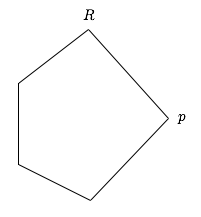
\includegraphics[width=1.5in]{diag.png} 
\end{figure}

Then notice we have $\htt p=1$, $\dim R/p=1$ but $\dim R=3$. 

\begin{dfn}[Catenary]
We say that $R$ is catenary if all saturated chains of primes between any two primes have the same length. Recall a saturated chain is one which cannot be refined. 
\end{dfn}

\begin{thmm}[Ratliff]
If $R$ is catenary then $\htt p+\dim R/p=\dim R$ for all primes $p \in \spec R$. Furthermore, any affine algebraic variety over a field is catenary. 
\end{thmm}

\noindent Proof: If $(f)$ is nonzero prime, then $(0) \subseteq (f)$ is a chain of length 1 so $\dim R \geq 1$. To show that $\dim R \leq 1$, we need to show that if $(f) \leq (g)$ for nonzero primes then we have equality, so we cannot extend the chain. Since $(f) \subseteq (g)$, then $f=rg$ for some $r$ so that $rg \in (f)$. As $(f)$ is prime, $r \in (f)$ or $g \in (f)$. We show that $r \notin (f)$: if $r=sf$, then $f=rg=sfg$ so that $(1-sg)f=0$. But then $f=0$, a contradiction. So $1-sg=0$ so that $1=sg$, showing that $(g)$ is not prime. \qed \\

Note that the converse is false as $\dim \Z[\sqrt{-5}]=1$ but this is not a UFD so that it is trivially not a PID. 

The first example of a non-catenary ring is due to Nagata in the 1950s and is not trivial. One should note that height was once called codimension and is still sometimes referred to as this - most notably in algebraic geometry. 

\begin{ex} To see some examples of this theorem:
\begin{enumerate}[(i)]
\item We have $\spec \Z=\{(0)\} \cup \{(p)\}_{p \text{ prime}}$. Each ideal $(p)$, where $p$ is prime, contains $(0)=\{0\}$ and no such ideal contains the other so that $\dim \Z=1$.

\item Generally, if $R$ is a PID that is not a field, then $\dim R=1$. 

\item If $k$ is a field then $\dim k=0$ (as it has a ``tiny" $\spec$). More generally, any artinian ring is 0-dimensional. 
\end{enumerate}
\end{ex}

Recall the following important result:

\begin{thmm}[Hopkins-Levitski Theorem]
Any artinian ring $R$ is noetherian. 
\end{thmm}

\begin{rem} There are a few important notes on the Hopkins-Levitski Theorem: 
\begin{enumerate}[(i)]
\item The converse of the Hopkins-Levitski Theorem: take $\Z$ or $k[x]$.
\item The Hopkins-Levitski Theorem is false for modules.
\item The proof of the Hopkins-Levitski Theorem shows more: if $R$ is an artinian ring:
\begin{itemize}
\item as a $R$-module, $R$ has finite length
\item $R$ has finitely many maximal ideals $\fm_1,\fm_2,\cdots,\fm_n$ and $J\defeq \cap \text{ max ideals}=\fm_1\cdots\fm_n$, where the last equality holds by the Chinese Remainder Theorem (if they are comaximal, this is obvious as they are maximal), and $J$ is nilpotent with $J=\nil R$. 
\end{itemize}
\end{enumerate}
\end{rem}

\begin{prop}
Let $R$ be a commutative noetherian ring, then $R$ is artinian if and only if $\dim R=0$.
\end{prop}

\noindent Proof: Assume that $R$ is artinian. By the Hopkins-Levinsky Theorem, $J$ is the jacobson radical of $R$. We know that $R$ has finitely many maximal ideals and $J$ is nilpotent. Then $J^s=0$ for some $s \geq 0$. Then we have $J^s \subseteq p$ for all $p \in \spec R$. This says that $J \subseteq p$. But we know that $J=\fm_1\cdots \fm_n$ so that $\fm_i \subseteq p$ for some $i$. Then $\spec R=\{\fm_1,\cdots,\fm_n\}$. In particular, there are no containments. 

If $\dim R=0$, then every prime ideal ideal is both maximal and minimal in $\spec R$. So every $p \in \spec R$ is a minimal prime of $(0)$. As $R$ is noetherian, the set $\spec R$ is finite. Suppose $\spec R=\{\fm_1,\cdots,\fm_n\}$. Then using Krull's Theorem, $\nil R=\cap_{p \in \spec R} p=\cap_{i=1}^n \fm_i=J$. In particular, we have $J=\fm_1\cdots\fm_n$ (by the Chinese Remainder Theorem). We have composition series for $R$
\[
R \supset \fm_1 \supset \fm_1 \fm_2 \supset \cdots J \supset J\fm_1 \supset J\fm_1\fm_2 \supset \cdots \supset J^2 \supset \cdots \supset J^s=0
\]
so that $R$ has finite length so that $R$ is artinian. \qed \\

\begin{ex}
$\dim(k[x_1,\cdots,x_n])=\dim \A_k^n=n$. To see that $\dim \geq n$, look at the inclusion $(0) \subsetneq (x_0) \subsetneq (x_0,x_1) \subsetneq \cdots \subsetneq (x_0,\cdots,x_n)$. To prove the other inequality, we need more theory.
\end{ex}

\begin{dfn}[Transcendence Basis]
Let $L/K$ be a field extension. A transcendence basis for an extension $L/K$ is a subset $B \subseteq L$ such that 
\begin{enumerate}[(i)]
\item $B$ is algebraically independent over $K$; that is, there does not exist a polynomial $f \in k[x_1,\cdots,x_n]$ such that $f(b_1,\cdots,b_n)=0$ for some $b_i \in B$. 
\item If $L$ is algebraic over $K(B)$.
\end{enumerate}
The cardinality of the basis $B$ is the transcendence degree of $L/K$, denoted $\tdeg(L/K)$ or $\tdeg_k(L)$.
\end{dfn}

One should show that this is uniquely defined - which it is - but we shall take this on faith. Observe that $\tdeg_k(L)$ is the cardinality of a maximal algebraic independent set.

\begin{ex}
Let $x_1,\cdots,x_n$ be indeterminant over $k$. We have $\tdeg_k k(x_1,\cdots,x_n)=n$. Then $k(x_1,\cdots,x_n)$ is purely transcendental over $k$, i.e. $L=K(B)$.
\end{ex}

\begin{ex}
If $L/K$ is an algebraic extension, then $\tdeg_k L=0$. 
\end{ex}

\begin{ex}
Let $S=k[x,y,z]$ and $f=xy-z^2 \in S$. One can show that $f$ is irreducible. Since $f$ is a UFD, we know that $f$ irreducible implies that $f$ is prime. So $R=k[x,y,z]/(f)$ is an integral domain. Set $L=Q(R)$. We claim that $\tdeg L/K=2$. Note that $Z(f) \subseteq \A_k^3$, the surface of a cone. To show this, we have $L=k(\ov{x},\ov{y},\ov{z})$ but not algebraically independent as $\ov{z}^2-\ov{x} \ov{y}=0$ in $L$. We shall show that $\{\ov{x},\ov{y}\}$ is a transcendence basis. Observe $L$ is algebraic over $k(\ov{x},\ov{y})$ since $\ov{z}$ is a root of $t^2-\ov{x}\ov{y}$. Then we have a $p(r,s) \in k(r,s)$ such that $p(\ov{x},\ov{y})=0$. But then $p(\ov{x},\ov{y})=\ov{p(x,y)}$. This means that $p(x,y)$ is a multiple of $(xy-z^2)$ in $k(x,y,z)$. But arguing by polynomial degree of $p(x,y)$ in $z$ that this is false so that $p(x,y)=0$.
\end{ex}

\begin{lem}[Lemma A]
Let $L/K$ be an algebraic field extension and $\alpha_1,\cdots,\alpha_n \in L$. Define $\phi: k[x_1,\cdots,x_n] \to L$ via $\phi(x_i)=\alpha_i$. Then $\ker \phi$ is a maximal ideal can be generated by $n$ polynomials $f_1(x_1),f_2(x_1,x_2),\cdots,f_n(x_1,\cdots,x_n)$ with each $f_i$ monic in $x_i$. 
\end{lem}

\noindent Proof: We know that $\im \phi$, $k[\alpha_1,\cdots,\alpha_n]$, is $k(\alpha_1,\cdots,\alpha_n)$ since each $\alpha_i$ is algebraic over $k$. This is a field so $k[x_1,\cdots,x_n]/\ker \phi \cong \im \phi$ so that $\ker \phi$ is a maximal ideal. We now construct the $f_i$'s inductively. 

Let $f_1(x_1)$ be the minimal polynomial of $\alpha_1$ over $k$. Then $k[\alpha_1] \cong k[x]/f_1(x)$, which is a field. This is isomorphic to $k(\alpha_1)$. Now $g_2(x) \in k(\alpha_1)[x]$ be the minimal polynomial for $\alpha_2$ over $k(\alpha_1)$. Since $k(\alpha_1)=k[\alpha_1]$, the coefficients of $g_2$ are polynomials in $\alpha_1$. So there is a $f_2(x_1,x_2) \in k[x_1,x_2]$ so that $k(\alpha_1,\alpha_2)=k(\alpha_1)[x_2]/f_2(\alpha_1,\alpha_2)$. We want to show that this is isomorphic to $k[x_1,\cdots,x_n]/(f_1,\cdots,f_n)$. Suppose that $p(x) \in \ker \phi$, i.e. $p(x_1,\cdots,x_n) \in k[x_1,\cdots,x_n]$ and $p(\alpha_1,\cdots,\alpha_n)=0$. 

We know that $f_n(\alpha_1,\cdots,\alpha_{n-1},x_n)$ be the minimal polynomial of $\alpha_n$ over a field $k(\alpha_1,\cdots,\alpha_{n-1})$. So $p$ is a multiple of $f_n$, i.e. $p(\alpha_1,\cdots,\alpha_{n-1},x) \in (f_n(\alpha_1,\cdots,\alpha_{n-1},x_n))$ as a polynomial in one variable $x_n$ over the field $k(\alpha_1,\cdots,\alpha_{n-1})$. Use the division algorithm for a polynomial in one variable in $k[x_1,\cdots,x_{n-1}]$ to write $p(x_1,\cdots,x_n)=q_nf_n+r_n$. Plugging in $x_i=\alpha_i$ for $i=1,2,\cdots,n-1$. We know that as $p(\alpha_1,\cdots,\alpha_{n-1},x) \in (f_n(\alpha_1,\cdots,\alpha_{n-1},x_n))$, we have $r_n=0$. But then $r_n(\alpha_1,\cdots,\alpha_{n-1},x_n)=0$. Then $r_n(\alpha_1,\cdots,\alpha_{n-2},x_{n-1},x_n) \in (f_{n-1}(x_1,\cdots,x_{n-1}))$ sine $k(\alpha_1,\cdots,\alpha_{n-1}) \cong k(\alpha_1,\cdots,\alpha_{n-2})[x_{n-1}]/(f_{n-1}(\alpha_1,\cdots,\alpha_{n-2},x_{n-1}))$. 

We repeat the argument, $r_n=q_{n-1}f_{n-1}+r_{n-1}$ as polynomials in $x_{n-1}$ over $k[x_1,\cdots,x_{n-2}]$ and plug in $\alpha_1,\cdots,\alpha_{n-2}$, et cetera. We get $p=q_nf_n+r_n,r_n=q_{n-1}f_{n-1}+r_{n-1},\cdots$. After $n$ steps, we have $p=\sum_{i=1}^n q_i+f_i+r_1(x_1,\cdots,x_n)$. So $r_1=0$ os that $p \in (f_1,\cdots,f_n)$. [Note that each step, $r_j(x_1,\cdots,x_n) \in (f_{j-1}(x_1,\cdots,x_{j-1}))$ after plugging in $\alpha_1,\cdots,\alpha_{j-2}$ so we write $r_j=q_{j-1}f_{j-1}+r_{j-1}$. So when $j=2$, we have $r_2 \in (f_1(x_1))$ and after plugging in 0 $\alpha$'s, we have $r_2=q_1f_1$.] \qed \\

\begin{lem}[Lemma B]
Let $k$ be a field and $R$ be a finitely generated $k$-algebra which is a domain. If $\tdeg_k Q(R)>0$ then $R$ is not a field. Therefore, if $R$ is a field then $\tdeg_k Q(R)=0$. 
\end{lem}

\noindent Proof: Let $\alpha_1,\cdots,\alpha_n \in R$ be elements which generate $R$ as an algebra over $k$. So we have $R=k[\alpha_1,\cdots,\alpha_n]$ and $Q(R)=k(\alpha_1,\cdots,\alpha_n)$. The set $\{\alpha_1,\cdots,\alpha_n\}$ contains a transcendence basis, say $\{\alpha_1,\cdots,\alpha_r\}$. Then $\{\alpha_{r+1},\cdots,\alpha_n\}$ are algebraic over the field $k[\alpha_1,\cdots,\alpha_r]=K$. By Lemma A, we can write $Q(R)=K[\alpha_{r+1},\cdots,x_n]/(f_{r+1}(x_{r+1}),\cdots,f_{n-r}(x_{r+1},\cdots,x_n))$. Set $d_i=\deg_{x_i} f_i$ for $i=r+1,\cdots,n$. Then $[k(\alpha_{r+1},\cdots,\alpha_{i+1}): k(\alpha_{r+1},\cdots,\alpha_i)]=d_i$. Now $K=k(\alpha_1,\cdots,\alpha_r)=Q(k[\alpha_1,\cdots,\alpha_r])$. So $k=k[\alpha_1,\cdots,\alpha_r]$ since they are transcendental. Coefficients in $K$ of the $f_i$'s have denominators in $k[\alpha_1,\cdots,\alpha_r]$. We get $g \in k[\alpha_1,\cdots,\alpha_r]$ so that $gf_i \in k[\alpha_1,\cdots,\alpha_r][x_{r+1},\cdots,x_n]$. Set $B=k[\alpha_1,\cdots,\alpha_r,1/g]$. 

We claim that $R[1/g]=B[\alpha_{r+1},\cdots,\alpha_r]$ is a finitely generated free $B$-module. We want to show that if $r>0$ then $R$ is not a field. If $R$ were a field then $g \in R$ so that $1/g \in R$ so that $R[1/g]=R$ is a finitely generated free $B$-module. But then $B$ cannot have any proper nonzero ideals. If it had one, $I \subseteq B$ is a proper nonzero ideal, then $IR=R$ as $R$ is a field so that $R/IR=0$. But by the above claim, $R/IR=B^n/IB^n \cong (B/I)^n \neq 0$ as $I$ is proper. Then $B$ is a field. Now $B$ contains a polynomial ring $k[\alpha_1,\cdots,\alpha_r]$ in $r$ variables so that it contains infinitely many irreducibles not dividing $g$. If $h$ is one of those then $1/h \notin k[\alpha_1,\cdots,\alpha_r,1/g]=B$ so that $B$ cannot be a field. If $r \geq 1$, then $B$ cannot be a field so that $R$ cannot be a field. 

It only remains to verify the claim. We show that $\{\alpha_{r+1}^{e_{r+1}},\alpha_{r+2}^{e_{r+2}},\cdots,\alpha_n^{e_n}\;|\; 0 \leq e_i<d_i\}$ is a basis for $R[1/g]$ over $R$. Every element of $R[1/g]$ is a basis of the form $p(\alpha_{r+1},\cdots,\alpha_n)$ for some $p(x_{r+1},\cdots,x_n) \in B[x_{r+1},\cdots,x_n] \subseteq k[x_{r+1},\cdots,x_n]$. If $\deg P$ in $x_i>d_i$, we can use the division algorithm (since $f_i$ is monic in $x_i$) to replace $p$ by something else equivalent of smaller degree equivalent module the $f$'s of smaller degree. Then this set spans $R[1/g]$. The basis is linearly independent over $k(\alpha_1,\cdots,\alpha_r)$, by more elementary field theory, hence over $R$ (by passing to the quotient field). \qed \\

\begin{thmm}
Let $R$ be a finitely generated algebraic extension over a field $k$ and assume $R$ is a domain. Then $\dim R=\tdeg_k Q(R)$.
\end{thmm}

\noindent Proof: Let $L=Q(R)$ and $r=\tdeg_k L$. Write $R=k[x_1,\cdots,x_n]/p$ for some $p \in \spec R$. First, we show that $r \geq \dim R$. It suffices to show $p \subsetneq q$ and $\tdeg_k Q(k[x_1,\cdots,x_n]/p) > \tdeg Q(k[x_1,\cdots,x_n]/q)$. We have a surjective map $k[x_1,\cdots,x_n]/p \to k[x_1,\cdots,x_n]/q$. So any transcendence basis for the left serves as a transcendence basis for the right as a generator up to an algebraic extension. Assume that equality holds. Write $k[x_1,\cdots,x_n]/p =k(\alpha_1,\cdots,\alpha_n)$. We have $k[x_1,\cdots,x_n]/q=k[\beta_1,\cdots,\beta_n]$. Assume that both fields have transcendence degree $r$ over $k$ and reorder the $\beta$'s such that the first $r$ of them form a transcendence basis. 

Then $\alpha_1,\cdots,\alpha_r$ are also a transcendence basis as any polynomial vanishing on $\alpha_1,\cdots,\alpha_r$ would vanish on the $\beta$'s. Set $W=k[x_1,\cdots,x_r] \setminus \{0\}$. We claim $p \cap W=q \cap Q=\emptyset$. If something is in the left side, we can plug in the $\alpha$'s to obtain that is 0. We get something similar on the right side by plugging in the $\beta$'s. So both $p,q$ survive in $k[x_1,\cdots,x_n]_W=k(x_1,\cdots,x_r)[x_{r+1},\cdots,x_n]$. But now 
\[
k[x_1,\cdots,x_n]_W/pk[x_1,\cdots,x_n]_W=(k[x_1,\cdots,x_n]/p)_W=k[\alpha_1,\cdots,\alpha_n]_W=k(\alpha_1,\cdots,\alpha_r)[\alpha_{r+1},\cdots,\alpha_n]
\]
But this is a field as $\alpha_{r+1},\cdots,\alpha_n$ are algebraic over $k(\alpha_1,\cdots,\alpha_r)$. So $p$ must be maximal in $k[x_1,\cdots,x_n]_W$, a contradiction. Then $p \subsetneq q$ and $q \cap W =\emptyset$ so that $r \geq \dim R$. 

We show $r \leq \dim R$ by induction on $r$. If $r=0$, then $R$ is a field by Lemma B or $r=0$ and $\dim R \geq 0$. If $r>0$, write $R=k[\alpha_1,\cdots,\alpha_n]$ with at least $\alpha_i$ transcendental over $k$. Set $W=k[x_1]\setminus \{0\}$. Write $R=k[x_1,\cdots,x_n]/p$. We know $W \cap p=\emptyset$ and $k[x_1,\cdots,x_n]_W=k(x_1)[x_2,\cdots,x_n]$ so 
\[
R_W=k[x_1,\cdots,x_n]_W/pk[x_1,\cdots,x_n]_W \cong k(\alpha_1)[\alpha_2,\cdots,\alpha_n] 
\]
has transcendental degree over $k(\alpha_1)$ one less, namely $r-1$. Then via induction we obtain $\dim(k[x_1,\cdots,x_n]_W/pk[x_1,\cdots,x_n]_W) \geq r-1$. Then we get a chain of primes in $k[x_1,\cdots,x_n]_W$ starting with $q_0 \defeq pk[x_1,\cdots,x_n]_W$, i.e. $q_1 \subsetneq \cdots \subsetneq q_{r-1}$. We look at their preimages in $k[x_1,\cdots,x_n]$
\[
p=p_0 \subsetneq p_1 \subsetneq \cdots \subsetneq p_{r-1}
\]
with $W \cap p_i = \emptyset$. In particular, $x_1 \notin p_i$ for all $i$. So the image of $x_1$ in $k[x_1,\cdots,x_n]/p_{r-1}$ which maps $\alpha_1$ in $R$ is transcendental. Then by Lemma B, $k[x_1,\cdots,x_n]/p_{r-1}$ is not a field. So $p_{r-1}$ is not maximal so we can extend the chain of primes $\{p_i\}_{i=1}^{r-1}$ by at least 1 more step. \qed \\

\begin{thmm}
Let $\fm$ be a maximal ideal of $k[x_1,\cdots,x_n]$ and $K=k[x_1,\cdots,x_n]/\fm$ be the residue field. Then $K$ is algebraic over $k$. Furthermore, by Lemma A, we can write $\fm=(f_1,\cdots,f_n)$ for polynomials $f_1,\cdots,f_n$. In particular, if $k$ algebraically closed then $\fm=(x_1-a_1,\cdots,x_n-a_n)$ for some point $(a_1,\cdots,a_n) \in \A_k^n$. 
\end{thmm}

\noindent Proof: Let $\alpha_1,\cdots,\alpha_n$ be the images of $x_1,\cdots,x_n$ in $k$. Then $K=k[\alpha_1,\cdots,\alpha_n]$ is a field. By Lemma B, $\tdeg_k B=0$, i.e. $K/k$ is algebraic. For the last assertion, suppose that $k=\ov{k}$. Then $k$ has no algebraic extension so $\ov{K}=K$. Then for all $i$, there is $a_i \in k$ such that $x_i \equiv a_i \mod \fm$. So $(x_1-a_1,\cdots,x_n-a_n) \subseteq \fm$, this is a maximal ideal as $k[x_1,\cdots,x_n]/(x_1-a_1,\cdots,x_n-a_n)$ (killing by this ideal, we have $k(a_1,\cdots,a_n)=k$) so that $\fm=(x_1-a_1,\cdots,x_n-a_n)$ by maximality. \qed \\

\subsection{Nullstellensatz}

\begin{thmm}[Hilbert's Nullstellensatz]
Let $k$ be an algebraically closed field. Then
\begin{enumerate}[(i)]
\item If $Z(I)=\emptyset$ for some $I \subseteq k[x_1,\cdots,x_n]$, then $1 \in I$.
\item $I(Z(I))=\sqrt{I}$
\end{enumerate}
\end{thmm}

\noindent Proof: 
\begin{enumerate}[(i)]
\item Suppose $1 \notin I$, i.e. $I \neq R$. Then $I$ is contained in some maximal ideal, $\fm$, i.e. $I \subset \fm$. By the preceding theorem, we know that $\fm=(x_1-a_1,\cdots,x_n-a_n)$. Then every polynomial in $I$ vanishes at the point $(a_1,\cdots,a_n)$ so that $Z(I) \neq \emptyset$. 

\item We know that $I \subseteq I(Z(I))$ and that $I(Z(I))$ is a radical ideal. So $\sqrt{I} \subseteq I(Z(I))$. We need only show the other containment. Let $f \in I(Z(I)) \subseteq k[x_1,\cdots,x_n]$. Consider the ideal $J=I+(1-yf) \in k[x_1,\cdots,x_n,Y]$ (this is called ``the trick of Ralomowitch"). If $p=(a_1,\cdots,a_n,b) \in \A_k^{n+1}$ is $Z(J)$ (notice this means that the points of $Z(J)$ never vanish on $I$ by the construction of $J$), then $(a_1,\cdots,a_n) \in Z(I)$. This shows $f(a_1,\cdots,a_n) \in Z(I)$. Then $(1-yf)(p)=1$, a contradiction to the fact that $p \in Z(J)$.

But then $J$ must be the whole ring, i.e. $J=k[x_1,\cdots,x_n]$. Then $1 \in J$ so we can write $1=\sum p_i(x_1,\cdots,x_n,Y)g_i(x_1,\cdots,x_n)+h(x_1,\cdots,x_n,y)(1-yf(x_1,\cdots,x_n))$. Putting in any number from $\A_k^n$ we always obtain a degree 0 piece (the 1 on the left side). Choosing additionally $y=1/f(x_1,\cdots,x_n)$ then $1=\sum p_i(x_1,\cdots,x_n,1/f(x))g_i(x_1,\cdots,x_n)$. Clearing denominators with a sufficiently large power of $f$, say $N$, we have $f^N=\sum p_i(x_1,\cdots,x_n)g_i(x_1,\cdots,x_n) \in I$.

\end{enumerate}
\qed \\

Now that we have shown the Nullstellensatz, we head towards our next long term goal: to prove the Krull Intersection Theorem (1930s). 

\subsection{Krull's Principle Ideal Theorem}

\begin{lem}[Krull's Principle Ideal Theorem, Base Case]
If $R$ is a noetherian ring and $x \in R$. Let $p$ be a minimal prime of $(x)$, i.e. $(x) \subseteq p$ and there is not $q$ with $(x) \subseteq p \subseteq p$. Then $\htt p \leq 1$. 
\end{lem}

\noindent Proof: Notice if $x$ is a unit, then $(x)=R$ and there are no such $p$'s. We can let $p$ be a minimal prime of $(x)$ (as $x$ is not a unit). If $p$ contains no primes, we are done. Assume $p \supsetneq q$. We want to show that $q$ has height 0, i.e. contains no other primes. Equivalently, show $\dim R_q=0$ (because the height is the same as the dimension of the localization). So we look at the reduction. In $R_p$, we still have $(x)R_p \subseteq pR_p$ and $qR_p \subset pR_p$. If we can show $qR_p$ has height 0, then $\htt q=0$. 

In other words, we may assume that $R$ is a local ring with unique maximal ideal $p$ (that is, localize and replace $R$ by $R_p$). Then in $R/(x)$ (this is the new $R$ - $R_p$), $p$ (the image of $p$) is maximal but also minimal over $(x)$. So there are no primes between $p$ and $x$. So $p$ is minimal in $R/(x)$. In particular, $\dim R/(x)=0$. Then $R/(x)$ is artinian. Recall the symbolic powers of $q$: $q^{(n)}\defeq q^nR_q \cap R$. Now $p$ is minimal over $(x)$ and $q \subset p$. In particular, $x \notin q$. Look at $q^{(n)}+(x)$. We then have $p \supset q^{(n)}+(x) \supset (x)$ and $p \supset q$. We know that $q^{(n+1)} \subseteq q^{(n)}$. So $q^{(n+1)}+(x) \subseteq q^{(n)}+(x)$. Since $R/(x)$ is artinian, this gives a descending chain of ideals which then must stabilize, say at $N$. 

Then $q^{(N+1)}+(x)=q^{(N)}+(x)$ for some $N$. So for every $f \in q^{(n)}$, there exists $g \in q^{(n+1)}$ and $a \in R$ such that $f=g+ax$. But then $ax=f-g \in q^{(N)}$. But $q^{(N)}$ is a primary ideal. So $a \in q^{(N)}$ or $x \in \sqrt{q^{(N)}}=q$ (that is, $x^N \in q^{(N)}$). But $x \in q$ yields a contradiction so that $a \in q^{(N)}$. So in fact, $q^{(N)} \subseteq q^{(N+1)}+q^{(N)}x$. In the ring $R/q^{(N+1)}$, this says $\ov{q^{(N)}} \subseteq \ov{q^{(N)}x}$. This is a problem as Nakayama's Lemma states that this only occurs if $\ov{q^{(N)}}=0$, i.e. $q^{(N)}=q^{(N+1)}$. Then $q^NR_q=q^{N+1}R_q$ so that by Nakayama's Lemma, $q^NR_q=0$. Then as this is a maximal ideal of $R_q$ and is nilpotent, $\dim R_q=0$, as desired. \qed \\

\begin{ex}
Let $R=k[x,y]/(x^2,xy,y^2)$. Then $\spec R=\{(x,y)\}$. In particular, $(x,y)$ is a maximal ideal but also minimal (over any element chosen) and has height 0.
\end{ex}

We now show the most general version of Krulls Principle Ideal Theorem. 

\begin{thmm}
Let $R$ be noetherian and $x_1,\cdots,x_n \in R$. Let $p$ be the minimal prime of $x_1,\cdots,x_n$. Then $\htt p \leq n$. 
\end{thmm}

\noindent Proof: We use the same reduction as before - localize at $p$ to assume that $R$ is local with maximal ideal $p$. Now as before $R/(x_1,\cdots,x_n)$ has only one prime ideal, so it is artinian. In particular, some power of $p$ (as the powers of $p$ form a descending sequence) is contained in $(x_1,\cdots,x_n)$ (as this sequence descends to 0 in $R/(x_1,\cdots,x_n)$). Let $q \subset p$. We have to show that $\htt q \leq n-1$. We shall show this via induction. We need to show that $q$ is minimal over some $(n-1)$-generated ideal: $(y_1,\cdots,y_{n-1})$. We may assume there are no primes between $p$ and $q$. 

As before, since $p$ is minimal over $(x_1,\cdots,x_n)$ and in fact one we have $x_i \notin q$ for some $i$. Renumber so that this $x_i$ is $x_n$. Then we look at $q+(x_n) \subset p$. We claim this is minimal over $p$. If $q+(x_n) \subset p' \subset p$, then $p'$ is between $q$ and $p$ so that $p'$ is minimal over $q+(x_n)$. But then in $R/q+(x_n)$, $\ov{p}$ is nilpotent. This forces $\ov{(x_1,\cdots,x_n)}$ to be nilpotent. So for $i=1,2,\cdots,n-1$, $x_i^t=y_i+a_ix^n$ and $a_i \in R$ and $y_i \in q$. Take $t$ sufficiently large show that all the $y$'s have this property. It remains to show that $q$ is minimal over $(y_1,\cdots,y_n)$. 

Observe that $y_i \in q$. Some power of $p$ is contained in $(x_1,\cdots,x_n)$ and some power of $(x_1,\cdots,x_n)$ is in $(y_1,\cdots,y_{n-1},y_n,x_n)$. Passing to $R/(y_1,\cdots,y_n)$, $\ov{p}$ is nilpotent. In $R/(y_1,\cdots,y_{n-1})$, $\ov{p}$ is minimal over $(x_n)$. By Krull's Theorem, this implies that $\ov{p}$ has height at most 1 in $R/(y_1,\cdots,y_n)$. But $\ov{q}$ is strictly contained in $\ov{p}$ so that $\htt \ov{q}=0$ in $R/(y_1,\cdots,y_{n-1})$. Hence, $q$ is maximal over $(y_1,\cdots,y_{n-1})$ in $R$. \qed \\

\begin{cor}
$\dim k[x_1,\cdots,x_n]=n$
\end{cor}

\noindent Proof: First, note that $\dim(k[x_1,\cdots,x_n]) \leq n$ as $\dim(k[x_1,\cdots,x_n])=\dim \A_k^n=n$. To see that $\dim \geq n$, look at the inclusion $(0) \subsetneq (x_0) \subsetneq (x_0,x_1) \subsetneq \cdots \subsetneq (x_0,\cdots,x_n)$. Lemma A implies that any maximal ideal of $k[x_1,\cdots,x_n]$ can be generated by polynomials $f_1,\cdots,f_n$ so any maximal ideal of $k[x_1,\cdots,x_n]$ has height at most $n$. \qed \\

\begin{cor}
If $R$ is noetherian and $p \in \spec R$ is an $r$-generated prime ideal, then $\htt p \leq r$.
\end{cor}

\begin{cor}
If $(R,\fm)$ is a local ring and $\fm$ is generated by $r$-elements then $\dim R \leq r$. 
\end{cor}

Before giving another useful fact about the dimension of $R$, we digress a bit on Nakayama's Lemma.

\begin{lem}[Nakayama]
Let $R$ be a commutative ring and $I \leq R$ an ideal with $I \leq \Jac(R)$. If $M$ is a finitely generated $R$-module with $M=IM$, then $M=0$. 
\end{lem}

It follows that if $N \subset M$ with $M=N+JM$, then $M=N$. To see this, apply Nakayama's Lemma to $M/N$. Namely, $J(M/N)=(JM+N)/N=M/N$ so that $M/N=0$ which implies $M=N$. Note also that if $(R,\fm)$ is a local ring and $M$ is generated by $x_1,\cdots,x_n$ such that $\ov{x}_1,\cdots,\ov{x}_n$ spans $M/\fm M$, then $x_1,\cdots,x_n$ generates $M$ as an $R$-module. To see this, we apply the previous comment to $N=\langle x_1,\cdots,x_n \rangle$. Then $M=N+\fm M$ so $M=N$. Finally, we note that $\mu_R(M)=\dim_{R/\fm}(M/\fm M)$ [from the previous comment, we get $\leq$. For $\geq$, note that $x_1,\cdots,x_n \in M$ generating $M$ also generate $M/\fm M$.] 

Returning to dimension, for a module $X$ over a local ring $(R,\fm)$, we define $\mu_R(x)$ (or sometimes $\nu_R(x)$) to be the minimal number of generators of $X$. By Nakayama's Lemma, this is $\dim_{R/\fm} (X/\fm X)$. We are then able to restate the corollary as

\begin{cor}
$\dim R \leq \dim_{R/\fm}(\fm/\fm^2)$
\end{cor}

\begin{dfn}[Embedding Dimension]
The embedding dimesion of $R$ is $\mu_R(\fm)=\dim_{R/\fm} \fm/\fm^2$.
\end{dfn}

Then the corollary says that the dimension of $R$ is at most the embedding dimension (think of a plane embedding in 3-space) and we have equality in the case of a regular local ring:

\begin{dfn}[Regular Local Ring]
If $R$ is a regular local ring $\dim R=\dim_{R/\fm}(\fm/\fm^2)$. 
\end{dfn}

\begin{ex} Examples of Regular Local Rings:
\begin{enumerate}[(i)]
\item $k$ a field
\item $\Z_{(p)}$
\item $k[x_1,\cdots,x_n]_{(x_1,\cdots,x_n)}$
\item $k[[x_1,\cdots,x_n]$
\end{enumerate}
There are ``all" the local rings (meaning, all the local rings one would ``meet in everyday life"). 
\end{ex}

We shall later show that a local ring $R$ is a regular local ring if and only if it has finite global dimension, i.e. every (finitely generated) $R$-module has finite projective dimension. 

\subsection{Dimension}

\begin{dfn}[Support]
Let $R$ be a ring and $M$ an $R$-module. The dimension of $M$, $\dim M$, is the combinatorial dimension of $\supp M$. As $\supp M \leq \spec R$, we have
\[
\dim M=\sup \{n\;|\; \text{there is a chain of primes }p_0 \subseteq \cdots \subseteq p_n \text{ with }M_{p_i}=0\}
\]
\end{dfn}

\begin{rem}
If $M$ is a finitely generated $R$-module, then $\supp M$ is a set of primes containing the annihilator:  $\supp M=V(\ann_R M)$. So $\dim M=\sup\{n\;|\; \text{ there is a chain } p_0 \subseteq \cdots \subseteq p_n  \text{ with }p_0>\ann_R M\}$ which is $\sup\{n\;|\; \text{ there is a chain } p_0 \subseteq \cdots \subseteq p_n  \text{ in }R/\ann_R M\}$ which is precisely $\dim(R/\ann_R M)$. So this says in some sense that the ring does not matter. We also have $\dim M \leq \dim R$.
\end{rem}

Note that if $p \in \supp M$ such that there is a chain of primes starting from $p$, i.e. $p_0=p$, and the chain has length $\dim M$, then $\dim M=\dim R/p \leq \dim R$. 

\begin{prop}
Let $(R,\fm)$ be a noetherian local ring and $M$ be a finitely generated $R$-module. Then for any $x \in R$, $\dim M/xM$ satisfies 
\[
\dim M-1 \leq \dim M/xM \leq \dim M
\]
\end{prop}

\noindent Proof: Since $\dim M=\dim R/\ann_R M$, we may assume first that $M=M/\ann_R M$ and then assume that $M=R$. So we need to show $\dim R-1 \leq \dim R/(x) \leq \dim R$. The fact that $\dim R/(x) \leq \dim R$ is clear as $\spec (R/(x))= V(x) \in \spec(R)$. For the left inequality, take elements $y_1,\cdots,y_l \in \fm$ so that in $R/(x)$, the maximal ideal $\ov{\fm}$ is minimal over $(\ov{y}_1,\cdots,\ov{y}_l)$ and $l$ the smallest possible such integer. We claim that $\fm$ is a minimal prime over $(y_1,\cdots,y_l,x)$ (Exercise). Then $\dim R\leq l+1$. \qed \\

Note in the above proof, we used the fact that in $(R,\fm)$, $\dim R=\sup\{l\;|\; \fm \text{ is a minimal prime of an }l-\text{generated ideal}\}$. We should show this:

\begin{prop}
Let $(R,\fm)$ be a noetherian local ring and $M$ be a finitely generated $R$-module. Then $\dim R=\sup\{l\;|\; \fm \text{ is a minimal prime of an }l-\text{generated ideal}\}$.
\end{prop}

\noindent Proof: Suppose that $M$ is minimal over $(x_1,\cdots,x_l)$. Then $\htt \fm \leq l$ by Krull's Principle Ideal Theorem. So $\dim R=\htt \fm \leq \sup\{l\;|\; \fm \text{ is a minimal prime of an }l-\text{generated ideal}\}$. For the other direction, we need find $x_1,\cdots,x_{\dim R}$ so that $\fm$ is minimal over $(x_1,\cdots,x_{\dim R})$. 

If $\dim R=0$, $\fm$ is a minimal ideal so that it is minimal over $(0)$. Now if $\dim R=1$, then $\fm \supset p_i$ for some possible infinite number of minimal primes $p_i$ and we have no other containments. But there must be finitely many as these minimal primes are associated and we know there are finitely many associated primes. Then $\spec R=\{\fm\} \cup \min R$. But $\min R \subseteq \ass R$, which is finite. 

We need find $x \in \fm$ so that $\fm$ is minimal over $(x)$, i.e. $(x)$ cannot be in the lower primes so $x \notin p_i$ for $i=1,2,\cdots,s$. So we only need show $\cup p+i \neq \fm$, but this is precisely prime avoidance. 

If $\dim R \geq 1$, take $\ov{\fm} \subset \fm$ with one less than $\htt \fm$. By induction, $\ov{\fm}$ is minimal over $(x_1,\cdots,x_{\dim R-1})$ for some $x_1,\cdots,x_{\dim R-1}$. Since the set of minimal primes of the ideal $(x_1,\cdots,x_{\dim R-1})$ is finite, we can find, using Prime Avoidance, $x_d \in \fm$ not in any minimal prime of $(x_1,\cdots,x_{\dim R-1})$. Then $\fm$ is the only prime containing all of $(x_1,\cdots,x_d)$. \qed \\

\begin{dfn}[System of Parameters]
Let $(R,\fm)$ be a noetherian local ring and $M$ be a finitely generated $R$-module of $\dim d$. A system of parameters for $M$ is a set of elements $x_1,\cdots,x_d$ such that $\dim(M/(x_1,\cdots,x_d)M)=0$. 
\end{dfn}

By the previous propositions, $d$ is the least possible. In the case of $M=R$, a system of parameters is a set $\{x_1,\cdots,x_{\dim R}\} \subset \fm$ such that $\fm$ is minimal over $(x_1,\cdots,x_{\dim R})$. 

\begin{ex}
Take $R=k[x,y,z]_{(x,y,z)}/(xz,yz)$. Geometrically, this is $Z(xz,yz) \subseteq \A^3_k$. Which is precisely $\{z=0\} \cup \{x=y=0\}$. Then pictorially, this is the $z$-axis through the $xy$-plane. We know that $R$ is a local ring with maximal ideal generated by $x,y,z$. It has embedding dimension $\mu_R(\fm)=\mu_R(x,y,z)=3$. Its primes are (canonically identified with) the primes in $k[x,y,z]_{(x,y,z)}$ containing $(xz,yz)$. We have the chain $(z) \subset (x,z) \subset (x,y,z)$ so that $\dim R \geq 2$. We claim that $\dim R=2$. We have $\{y,x-z\}$ as a system of parameters for $R$ so that $\dim R \leq 2$. To show this, it suffices to show that $R/(y,x-z)$ is 0-dimensional. But we have
\[
\begin{split}
R/(y,x-z)&=k[x,y,z]_{(x,y,z)}/(xz,yz,y,x-z) \\
&=k[x,y,z]_{(x,y,z)}/(y,xz,x-z) \\
&=k[x,y,z]_{(x,z)}/(xz,x-z) \\
&=k[x]_{(x)}/(x^2)
\end{split}
\]
so that this is 0-dimensional, as it has maximal ideal generated by $x$, which is nilpotent. 
\end{ex}

\subsection{Artin-Rees Lemma}

\begin{dfn}[Rees-Ring]
Let $R$ be a ring with $I \lhd R$. Then the Rees ring of $I$ is $R[It]$, which we think of as being in $R[t]$, where $It=\{at \;|\; a \in I\}$. 
\end{dfn}

\begin{rem}
There are a few things to note about Rees-rings:
\begin{enumerate}[(i)]
\item $R[It]=R+It+I^2t^2+\cdots$ is a graded ring.
\item If $I$ is finitely generated by $a_1,\cdots,a_r$ then $R=[It]=R[a_1t,\cdots,a_rt]$ is a finitely generated $R$-algebra. So if $R$ is noetherian, $R[It]$ is noetherian. 
\end{enumerate}
\end{rem}

\begin{ex}
Let $R=k[x,y]$ and $I=(x,y)$. We have $R[It]=R[xt,yt]$ is the homomorphic image of $R[u,v]$ given by $y \mapsto xt$ and $v \mapsto yt$. Then we have $yu \mapsto yt$ and $xv \mapsto xyt$. So we have $yu-xv \in \ker$. Then in fact one can check, $R[xt,yt] \cong R[u,v]/\ker = R[x,y,u,v]/(yu-xv)$. 
\end{ex}

\begin{rem}
If $M$ is any $R$-module, then $R[t] \otimes_R M$ is a $R[t]$-module. The elements are uniquely written as $1 \otimes x_0+t\otimes x_1+t^2 \otimes x_2+ \cdots + t^n \otimes x_n$, where $x_0,\cdots,x_n \in M$. We write this sum as $x_0+x_1t+\cdots+x_nt^n$. So we think of this tensor as $M[t]$. Then $R[t]$ has module structure on $M[t]$ given in the obvious way. 
\end{rem}

\begin{lem}[Artin-Rees Lemma]
Let $R$ be a noetherian ring and $N \leq M$ be finitely generated $R$-modules. Let $I$ be an ideal of $R$. Then there is a $c \geq 0$ such that $n \geq c$ so that 
\[
I^nM \cap N = I^{n-c}(I^cM \cap N)
\]
In other words, ``eventually" each submodule $N_{n+1}=I^{n+1}M \cap N$ satisfies $IN_n=N_{n+1}$. 
\end{lem}

\noindent Proof: Consider $M[t]=R[t] \otimes_R M$ and we look at the subset $\cM \defeq M+IMt+I^2Mt^2+\cdots \subseteq M+Mt+Mt^2+\cdots=M[t]$. Then $\mu$ is graded $R[It]$. Then $\cM=R[It]+R[It]x_1+R[It]x_2+\cdots+R[It]x_n$. We can think of $x_i$'s as in $M$ part of $\cM$. Set $\cN=N+(IM \cap N)t+(I^2M \cap N)t^2+\cdots \subset \cM$. 

Since $R[It]$ is noetherian, $\cM$ is finitely generated as an $R[It]$-module so that $\cN$ is generated by elements $(I^jM \cap N)t^j$ for $j \leq c$. Suppose $n \geq c$. The $\supseteq$ inclusion is obvious. We need only show $\subseteq$. Let $x \in I^nM \cap N$. We want to show that $x \in I^{n-c}(I^cM \cap N)$. Then $xt^n$ is in $(I^nM \cap N)t^n \leq \cN$. So $xt^n$ can be written as a sum of products $(a_kt^k)(x_jt^j)=a_kx_jt^{k+j}$, where $k+j=n, a_k \in R$, and $j<c$. So $x \in \sum_{j=1}^{c-1} I^{n-j}(I^jM \cap N)$ so that $I^nM \cap N=\sum_{j=1}^c I^{n-j}(I^jM \cap N)$. But these are nested:
\[
I^{n-j}(I^jM \cap N)=I^{n-c}I^{c-j}(I^jM \cap N) \subset I^{n-c}(I^jM \cap N)\subset I^{n-c}(I^c M \cap N)
\]
so that $I^nM \cap N \subseteq I^{n-c}(I^cM \cap N)$. \qed \\

This $c$ depends on $R,M,N,$ and $I$. The Uniform Artin-Rees Conjecture states there is a function $c=c(R,M,N)$ that does not depend on $I$. There are good partial results for this - see Huneks -- but the conjecture is still open. In terms of Cauchy sequence (a Cauchy sequence is a sequence of elements in a module and are said to converge with respect to $I$ if all eventual elements of the sequence ``land in" a power of $I$ - we define this rigorously later). Then the Artin-Rees lemma states, if $\{n_1,n_2,n_3,\cdots\}$ is a Cauchy sequence with respect to $I$ in $N$, then it is Cauchy with respect to $M$. We now turn to a use for the Artin-Rees Lemma:

\begin{thmm}[Krull Intersection Theorem - Baby Version]
Let $R$ be a noetherian ring and $I$ be an ideal of $R$ contained in $\Jac R$, then 
\[
\bigcap_{n \geq 0} I^n=(0)
\]
\end{thmm}

\noindent Proof: Set $N=\cap_{n \geq 0} I^n \leq R$. By the Artin-Rees Lemma, there is a $c \geq 0$ such that $I^nR \cap N=I^{n-c}(I^cR \cap N)$. We do not need the $R$'s here. So we can write $I^n \cap N=I^{n-c}(I^c \cap N)$. This shows that $N \leq IN$. But then $N=IN$. So by Nakayama's Lemma, $N=0$. \qed \\

This theorem simply states that Cauchy sequences converge. Now we look at a ``fancy" version of the Cayley-Hamilton Theorem:

\begin{thmm}
Let $R$ be a commutative ring and $M$ a $n$-generated module. Let $\phi: M \to M$ be a map such that $\phi(M) \subseteq IM$, where $I \lhd R$. Then $\phi$ satisfies an equation of the form
\[
\phi^n+a_1\phi^{n-1}+a_2\phi^{n-2}+\cdots+a_n 1=0
\]
in $\End_R(M)$ with $a_i \in I^i$. 
\end{thmm}

\noindent Proof: First, recall that for any commutative ing $R$ and any square matrix $A$ over $R$, there exists a square matrix of the same size $\text{adj } A$ such that $A\text{adj }A=\text{adj }AA=\det A I$, where here $\det A$ means the diagonal matrix whose entries have the value $\det A$. 

Now let $M$ be generated by $x_1,\cdots,x_n \in M$. Then by assumption, $\phi(x_j) \in IM$ for $j=1,2,\cdots,n$. So we have $\phi(x_j)=\sum_{i=1}^n a_{ij} x_i$ for some $a_{ij} \in I$ and $j=1,2,\cdots,n$. Let $A=(a_{ij})$ so that 
\[
A \begin{pmatrix} x_1 \\ x_2 \\ \vdots \\ x_n \end{pmatrix}=\begin{pmatrix} \phi(x_1) \\ \phi(x_2) \\ \vdots \\ \phi(x_n) \end{pmatrix}
\]
Then we have $(\phi-A) \mathbf{x}= \mathbf{0}$. [Note here we are mixing endomorphisms and morphisms] Let $B=\text{adj}(\phi-A)$. Then multiply by $B$ on the left to get 
\[
\begin{pmatrix} \det(\phi-A)x_1 \\ \det(\phi-A)x_2 \\ \vdots \\ \det(\phi-A)x_n \end{pmatrix} = \mathbf{0}
\]
In other words, $\det(\phi-A)$ is the annihilator of $M$. That means it is zero element of $\End_R(M)$ and it is a monic polynomial of degree $n$ in $\phi$ with coefficients from powers of $A$ so that $a_i \in I^i$. \qed \\

\begin{cor}
Let $R$ be a commutative ring and $M$ a finitely generated $R$-module. Let $I \unlhd R$ with $M=IM$. Then there is a $s \in I$ such that $(1-s)M=0$. 
\end{cor}

\noindent Proof: Take $\phi=1_M$ then $\phi^n+a_1\phi^{n-1}+\cdots+a_n 1_M=1_M+(-s)$, where $-s$ is a collection of elements of $I$. \qed \\

This proves Nakayama's Lemma: if $I \subseteq \Jac R$, the $1-s$ is a unit so $M=0$. 

\begin{thmm}[Krull's Intersection Theorem]
Let $R$ be a noetherian ring and $M$ a finitely generated $R$-module with $I \lhd R$. Then there is a $s \in I$ such that 
\[
(1-s) \bigcap_{n \geq 1} I^nM = 0
\]
In particular, if $I \subseteq \Jac R$, then $\cap_{n \geq 1} I^n M=0$.
\end{thmm}

\noindent Proof: By the Artin-Rees Lemma, we have 
\[
I \bigcap_{n \geq 1} I^nM = \bigcap_{n \geq 1} I^nM
\]
The theorem then follows from the proceeding corollary. \qed \\
% !TEX root = ../../commutative_algebra.tex

\newpage
\section{Completions}

\subsection{Inverse Limits}

Let $(\Lambda,\leq)$ be a poset. Assume that $\Lambda$ is directed; that is, for any $\lambda, \mu$, there is a $\nu \in \Lambda$ such that $\lambda \leq \nu, \mu \leq \nu$. 

\begin{ex}
Any totally ordered set, such as $\N$, is a directed poset. Furthermore, any set of subsets (or submodules) of a set (module) is a directed poset by ordering by containment or reverse containment. 
\end{ex}

An inverse limit system over $\Lambda$ is a set of objects (rings, modules, et cetera) $\{X_\lambda\}_{\lambda \in \Lambda}$ and maps (arrows) $\{f_{\lambda,\mu} : X_\mu \to X_\lambda, \lambda \leq \mu\}$ such that $f_{\lambda,\lambda}=1_{X_\lambda}$ and for $\lambda \leq \mu \leq \nu$, we have the following commutative diagram
\[
\begin{tikzcd}
X_\lambda & X_\mu \arrow[swap]{l}{f_{\lambda,\mu}} \\
& X_\nu \arrow[swap]{u}{f_{\mu,\nu}} \arrow{ul}{f_{\lambda,\nu}} 
\end{tikzcd}
\]

A candidate for an inverse limit of a system $\{X,f_{\lambda,\nu}\}$ is an object $X$ and maps $g_\lambda: X \to X_\lambda$ so that if $\lambda \leq \mu$ then the following diagram commutes
\[
\begin{tikzcd}
X \arrow{r}{g_\lambda} \arrow[swap]{d}{g_\mu} & X_\lambda \\
X_\mu \arrow[swap]{ur}{f_{\lambda,\mu}}
\end{tikzcd}
\]

A candidate $\{X,g_\lambda\}$ is an inverse if it has a universal property: 
 for all $X \in \text{obj } \mathcal{C}$ and morphisms $f_i: X \to M_i$ satisfying $\psi^j_i f_j=f_i$ for all $i \leq j$, there exists a unique morphism $\theta: X \to \plim M_i$ making the diagram commute
\[
\begin{tikzcd}
\plim M_i  \arrow{dr}{\alpha_i} \arrow[swap,bend right = 50]{ddr}{\alpha_j} & & X \arrow[dotted,swap]{ll}{\theta} \arrow[swap]{dl}{f_i}  \arrow[swap,bend left=50]{ddl}{f_j} \\
& M_i  & \\
&  M_j   \arrow{u}{\varphi^j_i} & 
\end{tikzcd}
\]

\begin{thmm}
Inverse limits exist over directed posets. 
\end{thmm}

The construction of $\plim X_\lambda$ is a subject of $\prod_{\lambda \in \Lambda} X_\lambda$ and we think of this as tuples $(x_\lambda)_{\lambda \in \Lambda}$
\[
\plim X_\lambda \left\{ (x_\lambda) \in \prod_{\lambda \in \Lambda} X_\lambda \;|\;  x_\lambda=f_{\lambda, \mu}(x_\mu) \text{ for } \lambda \leq \mu \right\}
\]

\begin{ex}
If $\Lambda=\N$ with the usual order $i \leq i+1$, then an inverse system is a sequence of objects $\{X_1,X_2,\cdots\}$ and maps $X_{i+k} \to X_i$ are determined by maps $X_{i+1} \to X_i$  via the commutating condition for inverse limits. The product $\prod_{i \in \N} X_i$ consists of sequences $(x_1,x_2,\cdots)$ with $x_i \in X_i$. Then we have
\[
\plim X_i= \{(x_1,x_2,\cdots)\;|\; x_i=f_{i,i+k}(x_{i+k}) \}=\{(x_1,x_2,\cdots,)\;|\; x_i=f_{i+1}(x_{i+1})\}
\]
We have the particular special case if all the maps $X_{i+1} \to X_i$ are surjective. Then we can build elements of the inverse limit system $\plim X_i$: choose $x_0$, then choose $x_1 \in f_{0,1}^{-1}(x_0)$, and so on. 
\end{ex}

\subsection{$I$-adic Completion}

Take a ring $R$ and $I$ an ideal of $R$. For $t \in \N$ consider the quotient $R/I^t$. Since $I^t \supseteq I^{t+1}$, we get a surjective homomorphism 
\[
R/I^{t+1} \to R/I^t
\]
so $\{R/I^t\}_{t \in \N}$ is an inverse limit system. 

\begin{dfn}[$I$-adic Completion]
The $I$-adic completion of $R$ is 
\[
\co{R}{I} \defeq \plim R/I^t
\]
\end{dfn}

The denotation $\co{R}{I}$ or just $\hat{R}$ if $I$ is understood. In particular, if $R$ is a local ring with maximal ideal $\fm$, then $\co{R}{\fm}$ is called \emph{the} completion of $R$. 

\begin{dfn}[Cauchy Sequence]
A sequence of elements of $R$, $r_0,r_1,\cdots$ is Cauchy with respect to an ideal $I$ if for $n \geq 0$, there is a $N \in \N$ such that if $i,j >N$, then $r_i-r_j \in I^t$. If $R$ is noetherian (so that Krull's Intersection Theorem holds) this is equivalent to the fact that $\{r_i\}$ is Cauchy with respect to the $I$-adic metric. 
\end{dfn}

\begin{dfn}[$C_I(R)$]
Define $C_I(R)$ to be the set of Cauchy sequences in $R$ with respect to $I$. This forms a ring under componentwise addition and multiplication. In fact, it is an $R$-algebra with $R \to C_I(R)$ given by $r \mapsto (r,r,r,\cdots)$ - the constant sequence. Define $C^0_I(R) \subset C_I(R)$ to be the Cauchy sequences converging to 0:
\[
C^0_I(R)=\{(r_0,r_1,\cdots) \;|\; \forall t \geq 0, \exists N \text{ so that if } i >N, \text{ then }r_i \in I^t\}
\]
\end{dfn}

\begin{prop}
$C_I^0(R)$ is an ideal of $C_I(R)$.
\end{prop}

\noindent Proof: $C_I^0(R)$ is an ideal of $C_I(R)$. Define for each $t$ a map $C_I(R) \to R/I^t$ as follows: for any sequence $(r_0,r_1,\cdots) \in C_I(R)$ and fixed $t$, the image of $r_i$ in $R/I^t$ is eventually independent of $i$ (this is Cauchy-ness: if $j>i$, then $r_j-r_i \in I^t$ so $r_j \equiv r_i$ in $I^t$) so we send a sequence $(r_0,r_1,\cdots)$ to that stable value. 

To show this map is onto, lift from $R/I^t$ to $R$ and its constant sequence. It is tedious to show that this is a ring homomorphism and that it kills $C_I^0(R)$ because its eventual value is $\ov{0}$. This gives a commutating triangle
\[
\begin{tikzcd}
C_I(R) \arrow{r} \arrow{d} & R/I^t \\
R/I^{t+1} \arrow{ur} & 
\end{tikzcd}
\]
So $C_I(R)/C^0_I(R)$ is a candidate for $\plim R/I^t$. So we get a ring homomorphism $C_I(R)/C_I^0(R) \to \plim R/I^t$. We only need show that this is bijective to show that it is an isomorphism. Give any sequence $(\ov{r}_0,\ov{r}_1,\ov{r}_2,\cdots)$ in the inverse limit, $\plim R/I^t$, we lift each $\ov{r}_i$ arbitrarily to $R$ then the result is Cauchy (by definition of $\plim R/I^t$) and the difference between any two lifted sequences is in $C_I^0(R)$. \qed \\

\begin{thmm}
Let $R$ be a ring and $I \lhd R$. Then completion $\co{R}{I} \cong C_I(R)/C_I^0(R)$ and the kernel of the natural ring homomorphism $R \to \co{R}{I}$ is $\cap_{n \geq 0} I^n$. In particular, if $R$ is noetherian then $R \to \co{R}{I}$ is injective by the Krull Intersection Theorem if $I \subset \Jac R$. 
\end{thmm}

\begin{ex}
Let $S$ be an arbitrary ring. Let $R=S[x_1,\cdots,x_n]$ with $I=(x_1,\cdots,x_n)R$. What is $\co{R}{I}$? Any element of $R/I^t$ can be represented as polynomials over $S$ of total degree at most $t-1$ of the $x_i$'s. So if a sequence $(\ov{f}_0,\ov{f}_1,\cdots)$ with $\ov{f}_i \in R/I^t$ represents an elements of the inverse limit, each $\ov{f}_t$ is the image of $\ov{f}_{t+k}$ under $R/I^{t+k} \to R/I^t$. In other words, the sum of the terms of degrees less than $t$ in $t+k$ is exactly $\ov{f}_t$. So if $n=1$, these look like $(s_0,s_0+s_1x,s_0+s_1x+s_2x^2,\cdots)$. So the limit is the power series $\sum_{i=0}^\infty s_ix^i$. We obtain a similar result for more than one variable: $\co{S[x_1,\cdots,x_n]}{(x_1,\cdots,x_n)}=S[[x_1,\cdots,x_n]]$. 
\end{ex}

In a sense, every example looks like this. Completing with respect to an ideal $I$ amounts to allowing power series in elements of $I$. Observe that if $R \ma{\phi} R'$ is a ring homomorphism and $I,I'$ are ideals of $R,R'$, respectively, with $I \to I'$, then we get an induced homomorphism $\co{R}{I} \ma{\ov{\phi}} \co{R'}{I'}$ as follows: take a Cauchy sequence $(r_0,r_1,\cdots)$ with respect to $I$, then the sequence $(\phi(r_0),\phi(r_1),\cdots)$ is Cauchy with respect to $I'$. Why? If $(r_0,r_1,\cdots,)$ is convergent to 0, then so too does $(\phi(r_0),\phi(r_1),\cdots)$. So $\ov{\phi}((r_0,r_1,\cdots)) \defeq (\phi(r_0),\phi(r_1),\cdots)$ works as a map. Even stronger, this induced homomorphism is functorial. Meaning, if $R_1 \ma{\phi_1} R_2 \ma{\phi_2} R_3$ with ideals $I_1,I_2,I_3$, receptively, mapping to each other, we get
\[
\begin{tikzcd}
\co{R_1}{I_1} \arrow{r}{\ov{\phi_1}} \arrow[swap]{d}{\ov{\phi_2\phi_1}} & \co{R_2}{I_2} \arrow{dl}{\ov{\phi_2}} \\
\co{R_3}{I_3} & 
\end{tikzcd}
\]
As a special case, if $\phi: R \to R'$ is surjective and $\phi(I)=I'$, then the induced homomorphism $\ov{\phi}$ is also surjective. 

\begin{prop}
Let $R$ be a noetherian ring and an ideal $I$ be generated by $a_1,\cdots,a_n$, then 
\[
\co{R}{I} \cong R[[x_1,\cdots,x_n]]/(x_1-a_1,\cdots,x_n-a_n)
\]
\end{prop}

\noindent Proof: Define $\phi: R[x_1,\cdots,x_n] \to R$ via $x_i \mapsto a_i$, then $\ker \phi$ is the given ideal: $\ker \phi=(x_1-a_1,\cdots,x_n-a_n)R[x_1,\cdots,x_n]$ so that we get $\ov{\phi}: \co{R[x_1,\cdots,x_n]}{(x_1,\cdots,x_n)} \to \co{R}{I}$ with kernel $(x_1-a_1,\cdots,x_n-a_n)R[[x_1,\cdots,x_n]]$. \qed \\

\begin{cor}
If $R$ is noetherian, so too is $\co{R}{I}$ is noetherian for all ideals $I$.
\end{cor}

By a variant of the Hilbert Basis Theorem, $R[[x]]$ is noetherian so that $\co{R}{I}$ is noetherian also. \qed \\

But why go through this process of completion? Well, the $\fm$-adic completion of a local ring $(R,\fm)$ is better because we get three important properties: Hensel's Lemma, Krull-Remack-Schmidt, and Cohen's Structure Theorem. We shall sketch proofs of both of these to varying levels. 

\begin{dfn}[Hensel's Lemma]
We say that a noetherian local ring $(R,\fm,k)$ satisfies Hensel's Lemma if for any monic polynomial $F(x) \in R[x]$ and any factorization mod $\fm$, $\ov{F}(x)=g(x)h(x)$ in $k[x]$ -- $k=R/\fm$ -- with $g(x),h(x)$ monic polynomials with $(g,h)=(1)$, there are monic polynomials $G,H \in R[x]$ with $\ov{G}=g,\ov{H}=h$, and $F=GH$. 
\end{dfn}

\begin{thmm}
Complete noetherian local rings $(R,\fm,k)$ satisfy Hensel's Lemma. 
\end{thmm}

\noindent Proof: Let $n=\deg F$, $r=\deg g$, and $n-r=\deg h$. We shall inductively construct $G_i(x)$ and $H_i(x)$ in $R[x]$ such that they are both monic with degree $r,n-r$, respectively. 
\begin{itemize}
\item $\ov{G}_i=g, \ov{H}=h$ in $k[x]$
\item $F \equiv G_iH_i$ mod $\fm^i[x]$.
\item This is unique: if $\ov{G}'_i=g,\ov{H}_i'=h$, and $F=G_i'H_i'$ mod $\fm^i[x]$, then $G_i \equiv G_i$ and $H_i' \equiv H_i$ modulo $\fm^i[x]$. 
\end{itemize}

Suppose we have shown the above. We shall show that the sequences of coefficients of $G_i$'s and $H_i$'s are Cauchy and so that $G,H$ have the desired properties. 

First, we show that the coefficients are Cauchy. If $i<j$, then $F \equiv G_jH_j \mod \fm^j [x]$ if and only if $F-G_jH_j \in \fm^j[x] \subset \fm^i[x]$ so that $F \equiv G_jH_j \mod \fm^i[x]$. By uniqueness, we have $G_i \equiv G_j$, $H_i \equiv H_j$ modulo $\fm^i[x]$ so that the sequences of coefficients are Cauchy. 

Now let $G(x),H(x)$ be the limits and write $G(x)=x^r+a_{r-1}x^{r-1}+\cdots+a_0$ and $H(x)=x^{n-r}+b_{n-r-1}x^{n-r-1}+\cdots+b_0$. Then $G \equiv G_j$ and $H \equiv H_j$ modulo $\fm^j[x]$ for all $j$. In particular, $\ov{G}=g$ and $\ov{H}=h$ modulo $\fm[x]$. We need to show that this product is the proper thing, i.e. $GH=F$. We look at the difference of the coefficients of $GH$ and $G_kH_k$: $(GH)_i-(G_\alpha H_\alpha)_i$
\[
\sum_{j=0}^i a_jb_{i-j} - \sum_{j=0}^i a_{kj} b_{k,i-j}= \sum a_j+b_{i-j}+a_{ki}b_{i-j}-a_{k,i}b_{i-j}-a_{kj}b_{k,-ij}=\sum (a_j-a_{k,j})b_{i-j} + (b_{i-j}-b_{k,i-j})a_{kj} 
\]
but $a_j-a_{kj} \in \fm^k$ and $b_{i-j}-b_{k,-ij} \in \fm^k$. So this is in $\fm^k$ so the sequence $G_kH_k \to GH$ coefficentwise. Then $F_i-(GH)_i=F_i-(G_kH_k)_i+(G_kH_k)_i-(GH)_i$. But $F_i-(G_kH_k)_i \in \fm^k$ and $(G_kH_k)_i-(GH)_i \in \fm^k$ for all $k$. Thus the coefficients of $F-GH$ are in $\cap_{k \geq 0} \fm^k=(0)$ (this is $(0)$ since $R$ is assumed noetherian so that Krull's Intersection Theorem applies). 

Now we need show that we can construct such things. Lift $g,h \in k[x]$ arbitrarily to $G_1,H_1 \in R[x]$ monic with degree $r,n-r$, respectively. Then $\ov{G}_1=g$ and $\ov{H}_1=h$ in $k[x]$ and since $gh=\ov{F}$, we have $F \equiv G_1H_1 \mod \fm[x]$. Suppose we have constructed up to $k$. Then we have $G_kH_k$ with $u_k(x),v_k(x)$ so that $u_k,v_k \in \fm^k[x]$ with $\deg u_k<r$ and $\deg v_k<n-r$. and so that $G_{k+1}(x)=G_k(x)+u_k(x)$ and $H_{k+1}(x)=H_k(x)+v_k(x)$ work. Now since $\gcd(g,h)=1$ in $k[x]$, we can find $p(x),q(x) \in R[x]$ so that $1=\ov{p}(x)g(x)+\ov{q}(x)h(x)$ in $k[x]$. But then $pG_k+qH_k \equiv 1 \mod \fm[x]$. 

Let $\Delta_k=F-G_kH_k \in \fm^k[x]$ by induction and $\deg \Delta_k <n$ since these are all monic. Then $\Delta_k \equiv \Delta_k(pG_k+qH_k) \mod \fm^{k+1}[x]=v_k(x)G_k(x)+u_k(x)H_k(x) \mod \fm^{k+1}[x]$. We may assume, since we are using the division algorithm for monic polynomials over $R/\fm^{k+1}$, that $\deg v_k<n-r$ and $\deg u_k<r$. Set $G_{k+1}=G_k+u_k$ and $H_{k+1}=H_k+v_k$ monic of the degree degrees. We need to check that $G_{k+1}H_{k+1} \equiv F \mod \fm^{k+1}[x]$. and $\ov{G}_{k+1}=g$ and $\ov{H}_{k+1}=h$ (which follows from the equivalences of $\Delta_k$ above). For uniqueness, this is an induction argument which occupies about 2 pages. \qed \\

\begin{ex}
As a non-example, take $R=\Z_{(7)}$ and $F(x)=x^2-2 \in R[x]$. Module the maximal ideal $(7)$, we have $\ov{F}(x)=x^2-\ov{2}=x^2-\ov{9}=(x-\ov{3})(x+\ov{3})$. But if the factorization lifted to $R$, then $F$ would have a root in $\Z_{(7)} \subseteq \Q$, a contradiction. 
\end{ex}

\begin{ex}
As another non-example, let $R=k[t]_{(t)}$ and $F(x)=x^2-t^3-t^2=x^2-t^2(t+1)$. Modulo $(t)$, this factors as $\ov{F}(x)=x^2$ but if $F$ factored, $R$ would contain $\sqrt{t+1}$ but it does not because of degree considerations. 
\end{ex}

\begin{ex}
Let $R=\Z_{(7)}$ and $\fm=(7)$. Then $\hat{R} \cong R[[x]]/(x-7)$. So in other words, ``power series in 7". Its elements are power series $a_0+a_17+a_27^2+\cdots$ with $a_k \in \Z$ and $0 \leq a_k<7$. We know that by Hensel's Lemma that $f(x)=x^2-2$ has a root in $\hat{R}$. In fact, we can write it down: $\sqrt{2}=3+1\cdot 7+2 \cdot 7^2+ 6 \cdot 7^3+\cdots$. Why? Partial sums differ from a root of $F$ by big powers of 7 and $(3+1 \cdot 7)(3+1 \cdot 7)=9+6 \cdot 7+1 \cdot 7^2=2+2 \cdot 7^2 \in (7)^2$.
\end{ex}

\begin{ex}
Set $R=\C[x,y]/(y^2-x^3-x^2)$. This gives the node. We know that $R$ is a domain since $y^2-x^3-x^2$ does not factor in $\C[x,y]$. If we complete at $\fm=(x,y)$, we get $\hat{R}=\C[x,y]/(y^2-x^3-x^2)$ and $x+1$ does not have a square root
\[
\sqrt{x+1}=1+\frac{1}{2} x-\frac{1}{8} x^2+\frac{1}{16} x^3-\frac{5}{32} x^4+ \cdots
\]
In particular, $\hat{R}$ is \emph{not} a domain. Completing zooms in at $(0,0)$ and we then see not one piece but two. We have $\hat{R} \cong \C[[u,v]]/(uv)$, where $u=y-x\sqrt{x+1}$ and $v=y+x\sqrt{x+1}$. 
\end{ex}

\begin{dfn}[Krull-Remack-Schmidt Property]
Let $\Lambda$ be a ring (not necessarily commutative). Say $\Lambda$ satisfies the Krull-Remack-Schmidt Proposition, if 
\begin{enumerate}[(i)]
\item Every left finitely generated $\Lambda$-module is a direct sum of indecomposable modules.
\item If $M=M_1\oplus \cdots \oplus M_r \cong N_1 \oplus \cdots \oplus N_s$ for indecomposable $\Lambda$-modules $M_i,N_j$, tehn $r=s$ and after possible permutation $M_i \cong N_i$ for all $i$. 
\end{enumerate}
\end{dfn}

\begin{prop}
Let $(R,\fm)$ be a local ring satisfying Hensel's Lemma. Then $R$ has the KRS property. 
\end{prop}

\begin{ex}
As a non-example, let $R=k[x,y]$, where $k$ is a field. Let $\fm=(x,y), \nu=(x-1,y)$. Then $\fm+\nu=R$ (as it has $x$ and $x-1$). So we get a short exact sequence
\[
0 \ma{} \fm \cap \nu \ma{} \fm \oplus \nu \ma{} R \ma{} 0
\]
where the final map is given by $(a,b) \mapsto a+b$ (or $a-b$). We know that $R$ is projective (as $R$ is free) so the sequence splits: $\fm \oplus \nu \cong R \oplus (\fm \cap \nu)$ but neither is free so that KRS property fails. 
\end{ex}

\begin{rem}
There are even examples of KRS failing over local rings. 
\end{rem}

\begin{cor}
Complete noetherian local rings have the KRS property. 
\end{cor}

\begin{cor}
Artinian local rings have the KRS property.
\end{cor}

\noindent Proof: Let $(R,\fm)$ be artinian. Then $J(R)=\fm$ is nilpotent so $\fm^t=0$. Then $\co{R}{\fm}=\plim R/\fm^t=R$. So artinian local rings are complete and noetherian. This then follows by the previous corollary. \qed \\

We have a nice structure theorem for complete local noetherian local rings.

\begin{dfn}
Let $(R,\fm,k)$ be a local ring.
\begin{enumerate}[(i)]
\item If $\ch R=\ch k$, $R$ is said to be equicharacteristic.
\item If $\ch R \neq \ch k$, $R$ is said to be mixed characteristic. In this situation, if $\ch R=0$ and $\ch k=p>0$. Then
\begin{enumerate}[(a)]
\item If $p \in \fm^2$, then $R$ is said to be ramified. 
\item If $p \in \fm \setminus \fm^2$, $R$ is said to be unramified. 
\end{enumerate}
\end{enumerate}
\end{dfn}

\begin{ex}
We have $R=\Q[[x_1,\cdots,x_n]], \F_p[[x_1,\cdots,x_n]], k[[x_1,\cdots,x_n]]$ as examples of an equicharacteristic ring. An examples of a unramified $R$, we have $\Z_{(p)}[[x_1,\cdots,x_n]], \co{\Z_{(p)}}{}$. As an of a ramified $R$, we have $\Z_{(p)}[[x]]/(x^2-p)$.
\end{ex}

\begin{thmm}[Cohen's Structure Theorem -- 1946]
Let $(R,\fm,k)$ be a complete regular local ring of dimension $d$. If $R$ is equicharacteristic then $R \cong k[[x_1,\cdots,x_d]]$ (so $R$ contains a copy of its own residue field). If $R$ is unramified, $R \cong V[[x_1,\cdots,x_d]]$ for some $V$, where $V$ is a one-dimensional complete regular local ring with maximal ideal generated by $p=\ch k$ ($V$ is a DVR -- a discrete valuation ring). Finally, if $R$ is ramified then $R \cong V[[x_1,\cdots,x_{d+1}]]/(f)$, where $V$ is as above and $f$ is a polynomial with nonzero constant term. 

Furthermore, any complete local noetherian ring is a homomorphic image of a complete regular local ring. 
\end{thmm}

\begin{cor}
Complete noetherian local rings are catenary, i.e. saturated chains of primes between any two fixed primes have the same length. 
\[
\dim R/p + \htt p= \dim R \;\;\;\;\; \forall p \in \spec R
\]
\end{cor}

\subsection{Completing Modules}

Let $R$ be a commutative ring with $I \lhd R$ an ideal. Let $M$ be an $R$-module. Recall that $C_I(R)$ is the set of Cauchy sequences of $R$ with respect to $I$. We define
\[
C_I(M)=\{(u_0,u_1,\cdots)\;|\; \forall t, \exists N \in \N \text{ such that } i,j>N, \text{ then }u_i-u_j \in I^tM\}
\]
This is a module over $C_I(R)$ under componentwise operations. Set $C_I^0(M)$ to be the set of Cauchy sequences that converge to 0, i.e.
\[
C_I^0(R)=\{(u_0,u_1,\cdots) \;|\; \forall t, \exists N \in \N \text{ such that }i>N, u_i \in I^tM\}
\]
This is a submodule of $C_I(R)$ and $\co{M}{I} \cong C_I(M)/C_I^0(M)$ is a module over $\co{R}{I} \cong C_I(R)/C_I^0(M)$. We could also define $\co{M}{I}= \plim M/I^tM$. We can then, as before, think of elements of $\co{M}{I}$ as sequences $(u_0,u_0+u_1,u_0+u_1+u_2,\cdots)$ with $u_t \in I^tM$ by passing to a subsequence of an arbitrary representative. 

Observe that completion is a functor from finitely generated $R$-mod to finitely generated $\co{R}{I}$-mod. If $f: M \to N$ is a $R$-homomorphism, then we obtain $C_I(f): C_I(M) \to C_I(N)$ given by $\{u_i\} \mapsto \{f(u_i)\}$. Then this morphism takes $C_I^0(M)$ into $C_I^0(N)$ so that we get an induced homomorphism $\hat{f}: \co{M}{I} \to \co{N}{I}$. 

\begin{prop}
Completion is an exact functor. That is, if 
\[
0 \ma{} A \ma{f} B \ma{g} C \ma{} 0
\]
is a short exact sequence of finitely generated $R$-modules, then
\[
0 \ma{} \co{A}{I} \ma{\hat{f}} \co{B}{I} \ma{\hat{g}} \co{C}{I} \ma{} 0
\]
is a short exact sequence of finitely generated $\hat{R}$-modules. 
\end{prop}

\noindent Proof: First, we show that $\hat{g}$ is surjective. Let $w \in \hat{C}$ be represented by $(w_0,w_0+w_1,\cdots)$ with $w_t \in I^tC$. Since $g: B \to C$ is onto, $I^tB$ maps onto $I^tC$ so that we can lift each $w_t$ to $v_t \in I^tB$. But then $(v_0,v_0+v_1,\cdots)$ is a Cauchy sequence in $B$ mapping to $w$. Now we show $\im \hat{f} \subseteq \ker \hat{g}$. We know that $\hat{g} \circ \hat{f}$ is defined by applying $g \circ f$ to each component of a Cauchy sequence. But $g \circ f=0$ so $\hat{g} \circ \hat{f}=0$. Observe that what we have done thus far has \emph{not} made use of noetherian or finitely generated. 

To see that $\hat{f}$ is injective, take $u \in \hat{A}$ and suppose $\hat{f}(u)=0$, where $u=(u_0,u_0+u_1,\cdots)$. Then the sequence $(f(u_0),f(u_0)+f(u_1),\cdots)$ is Cauchy in $B$ and converges to 0. But $(f(u_0),f(u_0)+f(u_1),\cdots)$ is contained in $f(A)$ so that this is Cauchy in $f(A)$ by the Artin-Rees Lemma. So $u=0$ as $f$ is injective. Finally, we need show $\ker \hat{g} \subseteq \im \hat{f}$. First, identify $A$ with its image in $B$ and $C=B/A$. Let $v \in \hat{B}$ map to 0 in $\hat{B/A}$. We will show that $v$ is represented by a sequence in $A$ so $v \in \hat{A}$. Write $v=(v_0,v_1,v_2,\cdots)$ with $v_{t+1}-v_t \in I^tB$ (by possibly passing to a subsequence if necessary). Since $v$ maps to 0 in $\hat{B/A}$, the sequence $(\ov{v}_0,\ov{v}_1,\ov{v}_2,\cdots)$, as elements in $B/A$, converges to 0. By possibly passing to a subsequence, we may assume $\ov{v}_t \in I^t(B/A)=\frac{I^tB+A}{A}$. So $v_t \in I^tB+A$. Write $v_t=z_t+a_t$ with $z_t \in I^tB$ and $a_t \in A$. Then the sequence $\{a_t\}$ is Cauchy with the same limit as $\{v_t\}$ since the difference is in $I^tB$. Then the sequence $(a_0,a_1,\cdots)$ represents $v$ and $v \in \hat{A}$. \qed \\

\begin{cor}
If $M$ is finitely generated over $R$, then $\co{M}{I}$ is finitely generated over $\co{R}{I}$ [Note: as commented in the previous proof, this does \emph{not} make use of $R$ noetherian.]
\end{cor}

\noindent Proof: Simply complete the surjection $R^n \to M \to 0$. \qed \\

\begin{rem}
There is a natural $R$-linear map $M \to \co{M}{I}$ given by $u \mapsto (u,u,\cdots)$ with $\ker= \cap_{t \geq 0} I^tM$. So $M \to \hat{M}$ is injective if $M$ is finitely generated and $I \subseteq J(R)$ by Krull's Intersection Theorem. 
\end{rem}

We say that $M$ is $I$-adically separated if $\cap_{t \geq 0} I^tM=0$. The map $m \to \co{M}{I}$ induces a $\co{R}{I}$-linear map $M \otimes_R \co{R}{I} \to \co{M}{I}$ via $u \otimes r_t \mapsto r_tu$.

\begin{prop}
This map is an isomorphism if $R$ is noetherian and $M$ is finitely generated.
\end{prop}

\noindent Proof: First, notice if $M=R$ then $R \otimes_R \hat{R} \to \hat{R}$, given by $r \otimes r_t \mapsto rr_t$, is an isomorphism. Furthermore, completion respects direct sums: $\hat{A \oplus B}=\hat{A} \oplus \hat{B}$: $((a_0,b_0),\cdots) \mapsto ((a_0,\cdots),(b_0,\cdots))$. But then the map $R^n \otimes_R \hat{R} \to \hat{R}^n$ is also an isomorphism. Let $M$ be an arbitrary finitely presented (as $R$ is noetherian) so we can write 
\[
R^m \ma{} R^n \ma{} M \ma{} 0
\]
Then we get a diagram 
\[
R^m \otimes \hat{R} \ma{} R^n \otimes_R \hat{R} \ma{} M \otimes_R \hat{R} \ma{} 0
\]

\[
\begin{tikzcd}
R^m \otimes \hat{R} \arrow{d} \arrow{r} & R^n \otimes_R \hat{R} \arrow{r} \arrow{d} & M \otimes_R \hat{R} \arrow{r} \arrow{d} & 0 \\
\hat{R}^m \arrow{r} & \hat{R}^n \arrow{r} & \hat{M} \arrow{r} & 0
\end{tikzcd}
\]
The top row is still exact since the tensor product is right exact. The bottom row is right exact as completion is an exact functor. The squares commute so the first and second vertical maps are isomorphisms and therefore the map $M \otimes_R \hat{R} \to \hat{M}$ is an isomorphism. \qed \\

\begin{rem}
This is true even if $M$ is not finitely generated. To prove this, write $M$ is a direct limit of finitely generated submodules and use the fact that the tensor product commutes with direct sums. 
\end{rem}

\begin{cor}
If $R$ is noetherian and $I\lhd R$, then $\co{R}{I}$ is a flat $R$-algebra. In the case where $(R,\fm)$ is local and $I=\fm$, $\hat{R}$ is faithfully flat, i.e. flat and if $M \otimes_R \hat{R} \to 0$ then $M=0$.
\end{cor}

\noindent Proof: The second part follows from an assigned exercise if $M$ is finitely generated or $M$ injects to $\co{M}{I}$. \qed \\

The most important special case is if $(R,\fm)$ is a noetherian local ring and $\hat{R}$ is the $\fm$-adic completion. 

\begin{prop} We have the following properties:
\begin{enumerate}[(i)]
\item $\hat{R}$ is a local ring with maximal ideal $\hat{\fm}=\fm \hat{R}$. In particular, $(\hat{\fm})^n=\fm \hat{R}$ for all $n$. 
\item For any $I \lhd R$, we have $\hat{I}=I \hat{R}$. In particular, we have $\hat{I}=I \hat{R}$ an ideal of $\hat{R}$.
\item There is a bijection between $\fm$-primary ideals and $\hat{\fm}$-primary ideals of $\hat{R}$ given by $I \to I\hat{R}$ and $J \to J \cap R$. 
\end{enumerate}
\end{prop}

\noindent Proof: 
\begin{enumerate}
\item[(ii)] We have an injective homomorphism $I \to R$. This induces a commutative triangle
\[
\begin{tikzcd}
I \otimes_R \hat{R} \arrow{r} \arrow{d} & R \otimes_R \hat{R}=\hat{R} \\
\hat{I} \arrow{ur} & 
\end{tikzcd}
\]
with two sides injective by the exactness of the completion. The third side is an isomorphism. Then the image of $I \otimes_R \hat{R}$ in $\hat{R}$ is $I \hat{R}$ so the image of $\hat{I}$ in $\hat{R}$ is also $I \hat{R}$. 

\item[(i)] Complete the short exact sequence 
\[
0 \ma{} \fm \ma{} R \ma{} k \ma{} 0
\]
where $k=R/\fm$ to get 
\[
0 \ma{} \hat{\fm} \ma{} \hat{R} \ma{} \hat{k} \ma{} 0
\]
But $\hat{k}=\hat{R/\fm}=\plim k/\fm^t k=k$. It then follows that $\hat{\fm}$ is a maximal ideal of $\hat{R}$. Notice that $\hat{\fm} \cap R=\fm \hat{R} \cap R$ contains $\fm$ but $\fm$ is maximal in $R$ so that we must have $\hat{\fm} \cap R=\fm$. But why is $\hat{\fm}$ the only maximal ideal of $\hat{R}$? Take $x \in \hat{R}$, say $x=(x_0,x_0+x_1,x_0+x_1+x_2,\cdots)$, where $x_t \in \fm^t$ for all $t$. Then $x \notin \hat{\fm}$ if and only if $x_0 \notin \fm$. Then $x_0$ is a unit so that $x_0+x_1$ is a unit, and so forth. Then $x_0+\cdots+x_t \notin \fm$ for all $t$. But then every entry of $x$ is a unit in $R$ so that $x$ is a unit in $\hat{R}$. But then the non-units form an ideal ($\hat{\fm}$ contains all non-units) so $\hat{R}$ is local. 

\item[(iii)] Observe that $I$ is $\fm$-primary if and only if $\sqrt{I}=\fm$ if and only if $\fm^n \subseteq I$ for some $n$. Then $\fm^n$ kills $R/I$, i.e. $\fm^n(R/I)=0$. So completing $R/I$,
\[
\hat{R/I}= \plim \frac{R/I}{\fm^t(R/I)}=R/I
\]
But then when we complete the short exact sequence
\[
0 \ma{} I \ma{} R \ma{} R/I \ma{} 0
\]
we get
\[
0 \ma{} \hat{I} \ma{} \hat{R} \ma{} R/I \ma{} 0
\]
which means $\hat{R}/\hat{I} \cong R/I$ and so 
\[
\hat{\fm}^n(\hat{R}/\hat{I})=\fm^n(\hat{R}/\hat{I})=\fm^n(R/I)=0
\]
so $\hat{I}$ is $\hat{\fm}$-primary ideal of $\hat{R}$. On the other hand, if $J$ is $\hat{\fm}$-primary, then $\hat{\fm}^n \subseteq J$ for some $n$. Then $\hat{\fm}^n \cap R \subseteq J \cap R$. We know that $\hat{\fm}^n \subseteq J \cap R$ so $J \cap R$ is $\fm$-primary. But then the $\fm$-primary ideals of $R$ containing $\fm^n$ correspond to the ideals of $R/\hat{\fm}^n$ which correspond to the ideals of $\hat{R}/\hat{\fm}^n$ which correspond to the $\hat{\fm}$-primary ideals of $\hat{R}$ containing $\hat{\fm}^n$. 
\end{enumerate}
\qed \\

We want to show that $\dim R=\dim \hat{R}$ for a local ring $R$. However, to show this we will need to digress to more theory. 

\subsection{Flatness}

Recall that an $R$-module $M$ is flat if $M \otimes_R -$ is an exact functor. 

\begin{dfn}[Flat Morphism]
If $\phi: R \to S$ is a ring homomorphism, we say that $\phi$ is flat (or $S$ is a flat $R$-algebra homomorphism) if $S$ is flat as an $R$-module. 
\end{dfn}

\begin{lem}
Let $R$ be a ring. 
\begin{enumerate}[(i)]
\item If $M$ is a flat $R$-module and $N_1,N_2 \leq N$ are submodules of a $R$-module $N$, then
\[
(N_1 \otimes_R M) \cap (N_2 \otimes_R M)=(N_1 \cap N_2) \otimes_R M
\]
as a submodule of $N \otimes_R M$.
\item If $\phi: R \to S$ is flat and $I_1,I_2 \unlhd R$ are ideals, then 
\[
I_1 S \cap I_2 S = (I_1 \cap I_2)S
\]
\end{enumerate}
\end{lem}

\noindent Proof: 
\begin{enumerate}[(i)]
\item Define $N \ma{f} N/N_1 \oplus N/N_2$ by $x \mapsto (\ov{x},\ov{x})$. Then for $f$, we have $\ker f = N_1 \cap N_2$. This gives an exact sequence
\[
0 \ma{} N_1 \cap N_2 \ma{} N \ma{} N/N_1 \oplus N/N_2
\]
Tensoring with $M$ is still exact
\[
0 \ma{} (N_1 \cap N_2) \times_R M \ma{} N \otimes_R M \ma{f \otimes 1} N/N_1 \otimes_R M \oplus N/N_2 \otimes_R M
\]
But then we have $\ker f \otimes 1=(N_1 \cap N_2) \otimes_R M=(N_1 \otimes M) \cap (N_2 \otimes_R M)$.

\item Notice that for any ideal of $R$, we have the exact sequence
\[
0 \ma{} I \ma{} R \ma{} R/I \ma{} 0
\]
Tensoring with $S$ gives an exact sequence of $S$-modules
\[
0 \ma{} I \otimes_R S \ma{} R \otimes_R S \ma{} R/I \otimes_R S \ma{} 0
\]
But this is precisely 
\[
0 \ma{} I \otimes_R S \ma{} S \ma{} S/IS \ma{} 0
\]
So analyzing kernels gievs $I \otimes_R S \cong IS$. The result then follows by applying (i) with $M=S$. 
\end{enumerate}
\qed \\

\begin{ex}
Let $R=k[t^2,t^3] \subseteq S=k[t]$. Then what is $t^2 R \cap t^3R$? Well, we know that $t^2R=\langle t^2,t^4,t^5,\cdots \rangle$ and $t^3R=\langle t^3,t^5,t^6,\cdots \rangle$. But then $t^2R \cap t^3R=\langle t^5,t^6,t^7$ so that $(t^2R \cap t^3R)S=t^5S$. On the other hand, $t^2S \cap t^3S=t^3S$ so that $\phi: R \to S$ is not a flat morphism. 
\end{ex}

Recall that a flat $R$-moudle $M$ is faithfully flat if $M \otimes_R N \neq 0$ for all $N \neq 0$ (this is slightly nonstandard). 

\begin{prop}
The following are equivalent for a flat $R$-module $M$:
\begin{enumerate}[(i)]
\item $M$ is faithfully flat
\item $M \otimes_R R/\fm \neq 0$ for all maximal $\fm$ of $R$
\item $\fm M \neq M$ for all maximal $\fm$ of $R$
\item For any $R$-linear $f: A \to B$, if $1 \otimes f: M \otimes_R A \to M \otimes_R B$ is injective then $f$ is injective. [This is the usual definition of faithfully flat.]
\end{enumerate}
\end{prop}

\noindent Proof: 
\begin{enumerate}[(i)]
\item[(i) $\to$ (ii):] Take $N=R/\fm$.
\item[(ii) $\to$(iii):] $M \otimes_R R/\fm=M/\fm M$.
\item[(iii) $\to$(i):] Since $N \neq 0$, take $x \in N \setminus \{0\}$. Let $\fm$ be the maximal ideal containing $\ann_R(x)$. Then $\ann_R(x)M \subseteq \fm M \neq M$ by assumption. So $M \otimes_R R/\ann_r(x) \neq 0$. But $R/\ann_R(x) \cong Rx \leq M$ via the map $1 \mapsto x$. So $M \otimes_R Rx\neq 0$ and $M \otimes_R Rx \subseteq M \otimes_R N$ by flatness so $M \otimes_R N \neq 0$. 
\item[(i)$\to$(iv):] Let $f: A \to B$ be given. Set $N=\ker f$. Then we have the exact sequence
\[
0 \ma{} N \ma{} A \ma{f} B
\]
Tensoring with $M$ preserves exactness
\[
0 \ma{} M \otimes_R N \ma{} M \otimes_R A \ma{1 \otimes f} M \otimes_R B
\]
If $1 \otimes f$ is injective, then $M \otimes_R N=0$ so that $N=0$ by faithfulness so that $f$ is injective. 
\item[(iv)$\to$(i):] If $M \otimes_R N=0$ for some $N$. Consider $f: N \to 0$. Then $1 \otimes f: M \otimes_R N \to M \otimes_R 0$ is injective so that $f$ is injective so that $N=0$. 
\end{enumerate}
\qed \\

\begin{cor}
Let $(R,\fm)$ and $(S,\eta)$ be local rings and $\phi: R \to S$ be a local ring homomorphism (that is, $\phi(\fm) \subseteq \eta$). Then $S$ is flat over $R$ if and only if $S$ is faithfully flat over $R$.
\end{cor}

\noindent Proof: $\fm S \subseteq \eta S \neq S$ so that we are done by (iii). \qed \\

\begin{prop}
Let $\phi: R \to S$ be a faithfully flat ring map. Then
\begin{enumerate}[(i)]
\item $_R M \to M \otimes_R S$ given by $x \mapsto x \otimes 1$ is injective. In particular, if $M=R$ then $\phi$ is injective. 
\item For all $I \unlhd R$, we have $IS \cap R=I$.
\end{enumerate}
\end{prop}

\noindent Proof: \\
\begin{enumerate}[(i)]
\item Take $0 \neq x \in M$. Then $Rx \leq M$. By faithfulness (as it preserves injections), we have $Rx \otimes_R S \leq M \otimes_R S$. But $Rx \otimes_R S=(x \otimes 1)S$. We know that $Rx \otimes_R S \neq 0$ by faithfulness so $x\otimes 1 \neq 0$. 
\item We apply (i) to $M=R/I$. We have $R/I \to R/I \otimes_R S=S/IS$ is injective. We know that the kernel of 
\[
R \to R/I \to R/IS
\]
is $I$ and is also $IS \cap R$. 
\end{enumerate}
\qed \\

\begin{rem}
Note that (ii) almost shows that if $\phi: R \to S$ is faithfully flat, then $\phi^\#: \spec S \to \spec R$ given by $q \mapsto q \cap R$ is surjective. However, this fails because extending prime ideals to a prime ideal is not necessarily prime....well, it is true but we need more to show it. 
\end{rem}

\begin{lem}
Let $R$ be a ring and $U$ a multiplicatively closed set. Let $M,N$ be $R_U$-modules. Then $M\times_{R_U} N =M \otimes_R N$. [We also have $M \otimes_{R/I} N=M\otimes_R N$ if $M,N$ are $R/I$-modules.]
\end{lem}

\noindent Proof: We know that being $R_U$-bilinear certainly implies $R$-bilinear. It remains to show for $x \otimes y \in M \otimes_R N$ and $r/u \in R_U$, then $\frac{r}{u}x \otimes y=x \otimes \frac{r}{u} y$. But this is routine
\[
\frac{r}{u} x \otimes y= \frac{r}{u} x \otimes \frac{u}{u} y=rx \otimes \frac{1}{u} y= x \otimes \frac{r}{u} y
\]
\qed \\

\begin{thmm}
If $\phi: R \to S$ is a map and $M$ is left $S$-module, the following are equivalent:
\begin{enumerate}[(i)]
\item $M$ is flat over $R$ as an $R$-module
\item $M_q$ is an $R_p$-module for all $q \in \spec S$ with $p=q \cap R$
\item $M_\eta$ is a $R_\fm$-module for all maximal $\eta \in \spec S$ with $\eta=\fm \cap R$
\end{enumerate}
Note that this shows flatness is a local property. 
\end{thmm}

\noindent Proof: \\
\begin{enumerate}
\item[(i) $\to$(ii):] Let $q \in \spec S$ and $p=q \cap R$. Then we have $\frac{\phi}{1}: R_p \to S_q$ via $\frac{r}{u} \mapsto \frac{\phi(r)}{\phi(u)}$ as $u \notin p$ then $\phi(u) \notin q$. So $M_q$ is a $S_q$-module hence an $R_p$-module via $\frac{\phi}{1}$. Then $- \otimes_{R_p} M_q$ makes sense. Then on $R_p$-modules using the previous lemma, we have $- \otimes_{R_p} M_q= - \otimes_R M_q=(-\otimes_R M) \otimes_S S_q$, which is a composition of two exact functors so that $M_q$ is flat over $R_p$. 
\item[(ii)$\to$(iii):] This is obvious. 
\item[(iii)$\to$(i):] Assume that $M_q$ is $R_p$-flat for maximal ideals $q \subseteq S$. Let $f: A \to B$ be an injective homomorphism of $R$-modules. We want to show that $1 \otimes f: A \otimes_R M \to B\otimes_R M$ is injective. Let $K=\ker f \otimes 1$. We will show that $K=0$. We have the exact sequence
\[
0 \ma{} K \ma{} A \otimes_R M \ma{1 \otimes f} B \otimes_R M
\]
So we have
\[
0 \ma{} K_q \ma{} (A \otimes_R M)_q \ma{f \otimes 1} (B \otimes_R M)_q=B \otimes_{R_p} M_q
\]
But
\[
\begin{split}
(A \otimes_R M)_q&=(A \otimes_R M) \otimes_S S_q \\
&=A \otimes_R M_q \\
&=A \otimes_R (R_p \otimes_{R_p} M_q) \\
&=A_p \otimes_{R_p} M_q
\end{split}
\]
so $K_q$ is the kernel of $f_p \otimes 1: A_p \otimes M_q \to B_p \otimes M_q$. Localization is flat so $A_p \to B_p$ is injective so that $f_p \otimes 1$ is injective so that $K_q=0$ for all maximal $q$ so that $K=0$. 
\end{enumerate}
\qed \\

Keep in mind that we are heading toward proving that faithfully flat maps give surjections on prime spectra. 

\subsection{Fibers}

Let $\phi: R \to S$ be a ring map and $p \in \spec R$. Then the fiber over $p$ is
\[
(\phi^\#)^{-1}(p)=\{q \in \spec S \;|\; \phi^{-1}(q)=p\}=\{q \;|\; q \cap R=p\}
\]
This set is homeomorphic to $\spec(S \otimes_R k(p))$, where $k(p)$ is the residue field of $R$ at $p$. That is, $k(p)=R_p/pR_p=(R/p)_{\ov{p}}$

\begin{prop}
\[
k(p)=R_p/pR_p=(R/p)_{\ov{p}}
\]
\end{prop}

\noindent Proof: Let $T=S \otimes_R k(p)$. Then we have
\[
\begin{split}
T&=S \otimes_R k(p) \\
&=S/pS \otimes_R R_p \\
&=(S/pS)_U
\end{split}
\]
where $U=\phi(R\setminus p)$. We have a map $\phi: S \to T$ given by $s \mapsto \ov{s} \in S/pS$. So we have a composition of quotient maps and localization. 
\[
\spec T \cong\{q \in \spec S\;|\; q \supset pS, q \cap \phi(R\setminus p)=\emptyset\}=\{q \;|\; q \cap R=p\}
\]
we only need prove the equality. To prove $\supseteq$, note that if $q \cap R=p$ then $pS \subseteq q$. If $x \in q \cap \phi(R \setminus p)$. But then $x \in q \cap \phi(R)=\phi(p)$, a contradiction. To see $\subseteq$, if we have $q \supseteq pS$ and $q \cap \phi(R \setminus p)=\emptyset$, then $q \cap R \supseteq pS \cap R \supseteq p$. If $x \notin p$ then $x \notin q \cap R$ so that $q \cap R \subseteq p$ so that it must be $p$. \qed \\

The fiber of $\phi: R \to S$ over $p \in \spec R$ is $S \otimes_R k(p)$. We showed that the spec of a fiber ring is the fiber of $\phi$ over $p$. 

\begin{ex}
If $R$ is a domain, then the prime $(0) \in \spec R$ is called the generic point as $\ov{(0)}=\spec R$. For a map $\phi: R \to S$, the generic fiber is a fiber over $(0)$, i.e. $\spec(S \otimes_R k((0))=S_U$, where $U=R \setminus\{0\}$. 
\end{ex}

\begin{ex}
Suppose that $(R,\fm)$ is a local ring. Then the closed fiber of a map $\phi: R \to S$ is a fiber over $\fm$. Recall that maximal ideals are only closed in the Zariski topology. Then $\spec(S \otimes_R k(\fm))=\spec(S/\fm S)$.
\end{ex}

\begin{ex}
If $(R,\fm)$ is a local ring and $\hat{R}$ the $\fm$-adic completion, the fibers of the map $R \to \hat{R}$ are called the formal fibers. The closed formal fiber is 
\[
\begin{split}
\hat{R} \otimes_R k(\fm) &= \hat{R} \otimes_R R/\fm \\
&= \hat{R}/\fm \hat{R} \\
&=R/\fm
\end{split}
\]
The generic formal fiber (if $R$ is a domain) is $\hat{R} \otimes_R Q(R)$. This can be very ugly indeed. 
\end{ex}

\begin{thmm}
Let $\phi: R \to S$ is a ring map and $M$ an $S$-module, then
\begin{enumerate}[(i)]
\item if $M$ is faithfully flat over $R$ then $\phi^\#(\supp M)=\spec R$. That is for all $p \in \spec R$, there is a $q \in \spec S$ such that $M_q \neq 0$ and $q \cap R=p$. 
\item If $M$ is a finitely generated $S$-module then $M$ is flat over $R$ and $\phi^\#(\supp M)$ contains all maximal ideals of $R$ if and only if $M$ is faithfully flat over $R$.
\end{enumerate}
\end{thmm}

\noindent Proof:
\begin{enumerate}[(i)]
\item Let $p \in \spec R$. Since $M$ is faithfully flat, we know $M \otimes_R k(p) \neq 0$. So set $T=S \otimes_R k(p)$. Then 
\[
\begin{split}
M' &\defeq M \otimes_R k(p) \\
&=M \otimes_S S \otimes_R k(p) \\
&= M \otimes_S T
\end{split}
\]
is a nonzero $T$-module. Let $\tilde{q} \in \spec T$ be such that $(M')_{\tilde{q}} \neq 0$ and set $q= \tilde{q} \cap S$. Then 
\[
\begin{split}
0 \neq (M')_{\tilde{q}} &=M' \otimes_S T_{\tilde{q}} \\
&=M \otimes_S (S_q \otimes_{S_q} T_{\tilde{q}} ) \\
&= M_q \otimes_{S_q} T_{\tilde{q}}
\end{split}
\]
So $M_q \neq 0$ and $q \cap R=\tilde{q} \cap R=p$.

\item This follows from (i). It is enough to show $M \otimes_R R/\fm \neq 0$ for all maximal $\fm \subset R$. Fix a maximal ideal $\fm$. By assumption, there is a $q \in \spec S$ with $q \cap R=\fm$ and $M_q \neq 0$. Since $M$ is finitely generated over $S$ so $M_q$ is finitely generated over $S_q$. Therefore by Nakayama's Lemma
\[
0 \neq M_q/qM_q =(M/q)_q
\]
So in particular, $M/qM \neq 0$. But $q \cap R=\fm$ so $\fm \subseteq q$ so $M/\fm M$ surjects to $M/qM$ so that $M/\fm M\neq 0$. 
\end{enumerate}
\qed \\

\begin{cor}
If $\phi: R \to S$ is faithfully flat, then $\phi^\#$ is surjective. 
\end{cor}

\begin{cor}
If $U$ is multiplicatively closed closed set in $R$ and $R \neq R_U$, then $R \to R_U$ is flat but never faithfully flat. 
\end{cor}

\noindent Proof: Inverting a nonunit $x \in R$ vaporizes maximal ideals containing $x$. \qed \\

\begin{cor}
If $(R,\fm)$ is local then $\dim R \leq \dim \hat{R}$.
\end{cor}


% !TEX root = ../../commutative_algebra.tex

\newpage
\section{Integral Extensions}

\begin{dfn}[Integral]
Let $R \subseteq S$ be commutative rings with identity. An element $s \in S$ is integral over $R$ if $s$ satisfies a monic polynomial in $S$ over $R$, i.e.
\[
s^n+r_1s^{n-1}+\cdots+r_{n-1}s+r_n=0
\]
for some $n \geq 0$ and $r_i \in R$. 
\end{dfn}

\begin{ex}
If $R,S$ are field, then $s \in S$ is integral over $R$ if and only if $s$ is algebraic over $R$.
\end{ex}

\begin{ex}
Take $R=k[t^2] \subseteq k[t]=S$. Then $t \in S$ is integral over $R$ since $t^2-t=0$. More clearly, $t$ is a root of $x^2-t^2 \in R[x]$. 
\end{ex}

\begin{ex}
Take $R=k[s^3,t^4] \subseteq k[s^3,t^4,st]=S$. Then $st$ is integral over $R$ as it is the root of $x^{12}-(s^3)^4(t^4)^3$. 
\end{ex}

\begin{rem}
Recall that if $R,S$ are both fields and $s \in S$ is algebraic over $R$ then $R(s)=R[s]$. We will prove something similar for integral elements. 
\end{rem}

\begin{prop}
Let $R \subset S$ and $u \in S$. Then the following are equivalent:
\begin{enumerate}[(i)]
\item $u$ is integral over $R$
\item $R[u]$ is a finitely generated $R$-module
\item there is a subring $B$ of $S$ with $R[u]\subseteq B \subseteq S$ which is a finitely generated $R$-module.
\item there is a faithful $R[u]$-module which is finitely generated over $R$
\end{enumerate}
\end{prop}

\begin{dfn}[Integral Extension]
A ring extension $R \subseteq S$ is an integral extension if every $s \in S$ is integral over $R$.
\end{dfn}

\begin{cor}
The following are equivalent for a ring extension $R \subset S$ and $u \in S$:
\begin{enumerate}[(i)]
\item $u$ is integral over $R$
\item $R[u]$ is a finitely generated $R$-module
\item $R \subseteq R[u]$ is an integral extension. 
\end{enumerate}
\end{cor}

\begin{rem}
If $R \subseteq S \subseteq T$ and $S$ is a finitely generated $R$ module and $T$ is a finitely generated $S$-module, then $T$ is a finitely generated $R$-module. This is simple enough to show: if $S$ is generated by $x_1,\cdots,x_n$ and $T$ is generated by $y_1,\cdots,y_m$, then $T$ is $\sum Rx_i y_j$. 
\end{rem}

\begin{cor}
Let $R \subseteq S$ be a ring extension and $u_1,\cdots,u_n \in S$. Then the following are equivalent:
\begin{enumerate}[(i)]
\item $u_1,\cdots,u_n$ are integral over $R$
\item $R[u_1,\cdots,u_n]$ is a finitely generated $R$-module
\item $R \subseteq R[u_1,\cdots,u_n]$ is integral
\end{enumerate}
\end{cor}

\begin{cor}
Let $S$ be a finitely generated $R$-algebra. Then $S$ is integral over $R$ if and only if $S$ is a finitely generated $R$-module. 
\end{cor}

\begin{ex}
Let $R=k[s^6,s^4t^2,s^2t^{112},t^{191}] \subseteq k[s,t]=S$. Now $S$ is generated as an $R$-algebra by $s,t$ which are both integral (look at $x^7-s^7, x^{191}-t^{191}$) so $R \subseteq S$ is integral by the corollary and hence the module is finitely generated. 
\end{ex}

\begin{dfn}
Let $R \subseteq S$ be rings. We say that $R$ is integrally closed in $S$ if no element of $S \setminus R$ is integral over $R$. 
\end{dfn}

\begin{prop}
Let $R \subseteq S$ be rings. Set $T=\{s \in S\;|\; s \text{ integral over }R\}$. Then 
\begin{enumerate}[(i)]
\item $T$ is a subring of $S$.
\item $T$ is integrally closed in $S$.
\end{enumerate}
$T$ is called the integral closure of $R$ in $S$.
\end{prop}

\noindent Proof: 
\begin{enumerate}[(i)]
\item It is enough to show that $T$ is closed under multiplication and addition. Let $u,v \in T$. Then $R[u,v] \subseteq T$ and $R[u,v]$ is a subring which is integral over $R$ so $u+v,uv \in T$. 

\item Take $u \in S$ to be integral over $T$. Then $u^n+t_1u^{n-1}+\cdots+t_n=0$ for some $t_i \in T$. Set $A=R[t_1,\cdots,t_n]$. Then $A$ is integral over $R$ and is finitely generated as an $R$-algebra. So $A$ is a finitely generated $R$-module. Similarly, $A[u]$ is integral over $A$ and a finitely generated $A$-algebra so it is a finitely generated $A$-module. But by a previous remark, $A[u]$ is a finitely generated $R$-module. But then $u$ is integral over $R$ and so $u \in T$.
\end{enumerate}
\qed \\

\begin{ex}[Classical Example]
Let $F$ be a number field (a finite algebraic extension of $\Q$). Let $R$ be the integral closure of $\Z$ in $F$ (an ``order"). We call this $R$ a ring of algebraic integers. 
\end{ex}

\begin{ex}
Let $F=\Q(i)$, then $R=\Z[i]$.
\end{ex}

\begin{ex}
Let $d \in \Z$ be squarefree and $F=\Q(\sqrt{d})$. Then 
\[
R=\Z[\sqrt{d}]= 
\begin{cases}
\Q(n), & d \equiv 2,3 \mod 4 \\
\Z\left[\frac{1+\sqrt{d}}{2}\right], & d \equiv 1 \mod 4
\end{cases}
\]
\end{ex}

\begin{dfn}
Let $R$ be a domain with fraction field $F$. We say that $R$ is integrally closed (or normal) if $R$ is integrally closed in $F$. 
\end{dfn}

\begin{prop}
UFDs are integrally closed (or normal)
\end{prop}

\noindent Proof: Let $R$ be a UFD with field of fraction $F$. Let $x/y \in F$ be integral over $R$ and be in reduced form. We have
\[
\left(\frac{x}{y}\right)^n+r_1\left(\frac{x}{y}\right)^{n-1}+\cdots+r_{n-1}\left(\frac{x}{y}\right)+r_n=0
\]
for $r_i \in R$. Clearing denominators yields
\[
x^n+(r_1y)x^{n-1}+\cdots+r_{n-1}y^{n-1}x+r_ny^n=0
\]
So $x^n$ is divisible by $y$ so that $y$ is a unit. But then $x/y \in R$. \qed \\

\begin{ex}
Both $\Z,k[x_1,\cdots,x_n]$ are normal. 
\end{ex}

\begin{ex}
Let $R$ be the integral closure of $\Z$ in $\Q(i)$. We clearly have $\Z[i] \subseteq R$. We also know that $\Z[i]$ is a Euclidean Domain, hence a UFD. But then $\Z[i]$ is integrally closed in $\Q(i)$. So any element $r \in R$ is integral over $\Z$ and hence integral over $\Z[i]$. But then it is integral in $\Z[i]$. Therefore, $R=\Z[i]$. 
\end{ex}

\begin{ex}
Let $R=k[s^2,st,t^3]$. Is $R$ normal or not? We need to identify the fraction field of $R \subseteq k[s,t]$. We know that $Q(R)\subseteq k(s,t)$ so that 
\[
\frac{1}{t}= \left( \frac{(st)^4}{(s^2)^2t^3} \right)^{-1} \in Q(R)
\]
and 
\[
\frac{1}{s}=\left( st \cdot \frac{1}{t} \right)^{-1} \in Q(R)
\]
so $Q(R)=k(s,t)$. But $s \in Q(R) \setminus R$ is a root of $x^2-s^2$ so that $R$ is not a normal. In fact, the integral closure of $R$ [in $Q(R)$] is the whole ring $k[s,t]$. 
\end{ex}

\subsection{Primes in Integral Extensions}

It is our goal now to show that $\dim R=\dim S$ if $R \subset S$ is integral. 

\begin{lem}
Let $R \subset S$ be an integral extension of domains. Then $R$ is a field if and only if $S$ is a field (if and only if $\dim =0$). 
\end{lem}

\noindent Proof: For the forward direction, suppose that $R$ is a field and $u \in S \setminus \{0\}$. We want to show that $u$ is a unit. We have $u^n+r_1u^{n-1}+\cdots+r_n=0$ for some $r_i \in R$. If $r_n=0$, we have $u(u^{n-1}+r_1u^{n-2}+\cdots r_{n-1}u)=0$. We can cancel $u$ and proceed inductively until we have shown $u$ is a unit. Therefore, we can assume without loss of generality that $r_n \neq 0$. But $r_n$ is a unit of $R$ and so we can write $u^n+r_1u^{n-1}+\cdots+r_{n-1}u= -r_n$. But the left is $u(u^{n-1}+r_1u^{n-2}+\cdots r_{n-1}u)$ so that $u$ is a unit. 

For the reverse direction, suppose that $S$ is a field. Let $r \in R \setminus \{0\}$. Then $0 \neq r \in R \subset S$ so that $r$ is a unit in $S$. So $1/r \in S$. But then $1/r$ is integral over $R$ so that 
\[
\left(\frac{1}{r} \right)^n+a_1\left(\frac{1}{r} \right)^{n-1}+\cdots+a_{n-1}\left(\frac{1}{r} \right)+a_n=0
\]
Clearing denominators, we have
\[
1+a_1 r+a_2r^2+\cdots+a_{n-1}r^{n-1}+a_nr^n=0
\]
But then $-1=r(a_1+a_2r+\cdots+a_n r^{n-1})$ so that $r$ is a unit. \qed \\

\begin{lem}
Let $R \subseteq S$ be an integral extension and $I \subseteq S$ an ideal. If $U \subseteq R$ is multiplicatively closed then
\begin{enumerate}[(i)]
\item $R/I \cap R \subseteq S/I$ is integral 
\item $R_U \subseteq S_U$ is integral 
\end{enumerate}
\end{lem}

\noindent Proof: We prove (i). Let $\ov{u}=u+I \in S/I$. Then $u$ is integral over $R$ so that $u^n+r_1u^{n-1}+\cdots+r_n=0$. Passing to $S/I$, we get 
\[
\ov{u}^n+\ov{r}_1 \ov{u}^{n-1}+\cdots+\ov{r}_n=0
\]
so that $\ov{u}$ is integral over $R/I \cap R$. \qed \\

\begin{cor}
Let $R \subseteq S$ be an integral extension and $q \in \spec S$. Then $q$ is maximal if and only if $q \cap R$ is maximal. 
\end{cor}

\noindent Proof: By the lemma, we know that $R/q \cap R \subseteq S/q$ is integral and they are both domains. So by the other lemma, we know that $q \cap R$ is maximal if and only if $R/q \cap R$ is a field which is equivalent to $S/q$ being a field which is equivalent to $q$ being maximal. 

\subsection{Lying Over}

\begin{thmm}[Cohen-Seidenberg Lying Over]
Let $R \subseteq S$ be an integral extension and $p \in \spec R$. Then there is a $q \in \spec S$ lying over $p$, i.e. $q \cap R=p$. 
\end{thmm}

\noindent Proof: First, we localize. Let $U=R \setminus p$. Then $R_U \subseteq S_U$ is integral by the lemma and $R_U=R_p$ is local with maximal ideal $p$. Choose any maximal ideal $q \in S_U$. We know that $\spec S_U=\{q \in \spec S \;|\; q \cap U=\emptyset\}$. We claim that $q_U \cap R_U=(q \cap R)_U$ for any $q \in \spec S$. If we can only prove this, we will be done as we know that if $q_U$ is maximal then $q_U \cap R_U$ is maximal in $R_U$ so that $q_U \cap R_U=p$ so that $(q \cap R)_U=p$ showing $q \cap R=p$. We need show the claim. We have an exact sequence
\[
0 \ma{} R/q \cap R \ma{} S/q
\]
Localizing gives
\[
0 \ma{} (R/q \cap R)_U \ma{} (S/q)_U
\]
which is
\[
0 \ma{} R_U/(q \cap R)_U \ma{} S_U/q_U
\]
But the kernel is precisely $q_U \cap R_U$ so that $q_U \cap R_U=(q\cap R)_U$. \qed \\

\begin{lem}[Incomparable]
Let $R \subseteq S$ be an integral extension and $q \subsetneq Q$ be primes of $S$. Then $q \cap R \subsetneq Q \cap R$.
\end{lem}

\noindent Proof: Clearly $q \cap R \subseteq Q \cap R$. Suppose that $q \cap R = Q \cap R=p \in \spec R$. Set $U=R \setminus p$ and localize at $U$. We know that $P_U= pR_p$ is the unique maximal ideal of $R_U$ and $S_U$ is integral over $R_U$. But $q_U \cap R_U=(q \cap R)_U=p_U$ and $Q_U \cap R_U=(Q \cap R)_U=Q_U$ so that $q_U$ and $Q_U$ are maximal ideals of $S_U$. But $q_U \subseteq Q_U$ so that $q_U=Q_U$ so that $q=Q$. \qed \\

\begin{cor}
If $q \neq q'$ satisfy $q \cap R = q' \cap R$, then $q,q'$ are incomparable; that is, neither $q \subseteq q'$ nor $q' \subseteq q$. 
\end{cor}

\begin{lem}[Going Up]
Let $R \subseteq S$ be an integral extension with $p \subsetneq P$ primes of $R$. Assume that $q$ is a prime of $S$ lying over $p$. Then there exists a $Q \in \spec S$ with $Q \supsetneq q$ and $Q \cap R=P$. 
\end{lem}

\noindent Proof: Set $U=R \setminus P$ and localize at $U$ (this is because we do not care about primes bigger than $P$ so we may as well blow them away). We know $R_U=R_P \subseteq S_U$ is an integral extension and $PR_P$ is the unique maximal ideal. We have $q_U \in \spec S_U$. Choose any maximal ideal $Q_U$ of $S_U$ containing $q_U$. Then $Q_U \cap R_U$ is maximal in $R_U$ so that $Q_U \cap R_U =P_U$. Hence $Q \cap R=P$ by the one-to-one correspondence for $\spec$ of localizations. We need $Q \supsetneq q$ and we have $Q \supseteq q$ by choice of $Q_U$. If $Q=q$ then $q \cap R=Q \cap R$ so that $P=p$, a contradiction. \qed \\

A natural question is if (faithfully) flat extensions have the Going Up property. The answer is no. Take $R=\Z$ and $S=\Z[x]$. This is faithfully flat. Take $q=(1+2x)S$ so that $q \cap \Z=(0)=P$ (as $q$ has no constants) and then $P=(2)R$. If going up held there would be a $Q \in \spec S$ with $Q \cap \Z=(2)$ and $1+2x \in Q$. If $Q \cap \Z=(2)$ then $2x \in Q$ then $2 \in Q$ so that $1 \in Q$ as $1=(1+2x)-2x$. But then $Q \cap \Z=\Z$, a contradiction. 

\begin{thmm}
Let $R \subseteq S$ be a ring extension satisfying Lying Over, Going Up, and Incomparable. Then $\dim R=\dim S$. 
\end{thmm}

\noindent Proof: We need show both inequalities. To show $\leq$, let $p_0 \subsetneq p_1 \subsetneq \cdots \subsetneq p_n$ be primes in $R$. By Lying Over, there is a $q_0 \in \spec S$ with $q_0 \cap R =p_0$. By Going Up, we get a chain of distinct primes $q_0 \subseteq q_1 \subseteq \cdots \subseteq q_n$ in $S$ so that $n \leq \dim S$. 

To see $\geq$, let $Q_0 \subseteq \cdots \subseteq Q_n$ be a chain of primes in $S$. When we collapse down to $R$, by Incomparable, nothing collapses so we get a chain $p_0 \subsetneq p_1 \subsetneq \cdots \subsetneq p_n$ with $Q_i \cap R=p_i$. \qed \\

\begin{ex}
Any ring of algebraic integers, i.e. $\Z$ in a number field, has dimension 1 since it is integral over $\Z$. Specific examples include $\Z[i]$ and $\Z\left[\frac{1+\sqrt{2}}{2}\right]$. 
\end{ex} 

\begin{ex}
We know that $k[s^9,s^6t^2,st^{103},t^{11111}]$ has dimension 2 since $k[s,t]$ is integral over it. 
\end{ex}

\begin{prop}
If $R \subseteq S$, where $S$ is noetherian, is an integral extension then $\phi^\#: \spec S \to \spec R$ is a finite mapping, i.e. finite to one. 
\end{prop}

\noindent Proof: We know by Lying Over that there is at least one $q$. Then $p \subseteq pS \cap R \subseteq q \cap R=p$ so that we must have all equalities which gives $p(S \cap R)=p$. We claim the $q$'s lying over $p$ are all minimal over $pS$. To see this, if $pS \subseteq q \subsetneq q$ and $q' \cap R=p$, then we would have $q \cap R=p$ as well. By Incomparable, we must have equality so that there are only finitely many $q$'s since the minimal primes of $pS$ is a finite set. \qed \\

Furthermore, Zariski's Main Theorem states that any ring homomorphism inducing a finite mapping on $\spec$ is a composition of localization and integral extensions. But this theorem is very deep and very hard. 

\begin{dfn}[Going Down]
A ring extension $R \subseteq S$ satisfies Going Down if given any primes $p \subsetneq P$ of $R$ and any $Q \in \spec S$ lying over $p$, there is a $q \subsetneq Q$ with $q \cap R=p$. 
\end{dfn}

\begin{rem}
Arbitrary integral extensions do not satisfy this. For example, take $R=k[s] \subseteq k[x,y]/(xy,y^2-y)$. Then this is an integral extension since it is generated by $y$ and $y$ is a root of $y^2-y$, i.e. $t^2-t \in R[t]$. But Going Down fails. Set $p=(0) \subsetneq P=(x)$ and $Q=(1-y)S$. Notice that $Q \supset (x)=P$ since $x=x(1-y)$ as $xy=0$. So $Q \cap R \supset P$ and $P$ is maximal so that $Q \cap R=P$. However, $Q$ is also a minimal prime ideal of $S$. If $q \subsetneq Q$ then $1-y \notin q$. It cannot contain $y$ since then $Q$ would contain 1. But it has to contain $y^2-y=y(1-y)$ so it contains one or the other. But then no such $q$ exists to satisfy Going Down. 
\end{rem}

\begin{rem}
Going Down still fails to hold in arbitrary integral extensions even if $R,S$ are assumed to be domains. You need more still.
\end{rem}

\begin{thmm}
Let $R \subseteq S$ be and integral extension, where $R,S$ are both integral domains with $R$ normal. Then $R \subseteq S$ satisfies Going Down.
\end{thmm}

\begin{prop}
Let $\phi: R \to S$ be a flat ring homomorphism. Then $\phi$ satisfies Going Down.
\end{prop}

\noindent Proof: Let $p \subsetneq P$ be primes in $R$ and $Q \in \spec S$ lying over $P$. Localize at $P,Q$: $\frac{\phi}{1}: R_p \to S_Q$ is a flat local ring homomorphism. Hence, $\frac{\phi}{1}$ is faithfully flat. So $\left(\frac{\phi}{1}\right)^\#: \spec S_Q \to \spec R_P$ is surjective. Then there is a $q_Q$ lying over $p_P$. Hence, $q$ lies over $p$. \qed \\

\begin{lem}
Let $(R,\fm)$ be a noetherian local ring. Then there is a system of parameters for $R$; that is, elements $x_1,\cdots,x_d \in \fm$ with $d=\dim R$ and $\sqrt{(x_1,\cdots,x_d)}=\fm$. 
\end{lem}

\noindent Proof: We proceed by induction on $d=\dim R$. If $d=0$ then $R$ is artinian so $\fm$ is nilpotent. So $\fm=\sqrt{(0)}$ is generated by 0 elements. Now assume that $d \geq 1$ and $p_1,\cdots,p_s$ are primes of $R$ such that $\dim R/p_i=\dim R$ (these are minimal primes that occur in chains of maximal length). Since $d \geq 1$ and $\dim R/\fm=0$, $\fm$ is not among the $p_i$'s. So $\fm \subsetneq \bigcup_{i=1}^s p_i$ by Prime Avoidance. Take $x_1 \in \fm$ so that $x_1 \notin p_i$ for all $i$. Then $\dim R/(x_1) < \dim R$ (we know that $\dim R/(x_1) \geq \dim R-1$ so it must be equal to it). Then it follows by induction that there are $x_2,\cdots,x_d$ such that $\sqrt{(\ov{x}_2,\cdots,\ov{x}_d)}= \ov{\fm}$ so $\sqrt{x_1,\cdots,x_d}=\fm$. \qed \\

\begin{lem}
Let $(R,\fm)$ be a noetherian local ring. If $\sqrt{(x_1,\cdots,x_t)}=\fm$, then $t \geq d$. 
\end{lem}

\noindent Proof: We know that the dimension drops by 1 each time and $\sqrt{(x_1,\cdots,x_n)}=\fm$ if and only if $\fm^n \subseteq (x_1,\cdots,x_n)$ for some $n$ if and only if $R/(x_1,\cdots,x_n)$ is artinian, i.e. 0-dimensional. \qed \\

\begin{thmm}
Let $\phi: R \to S$ be a homomorphism of noetherian rings and $q \in \spec S$ with $p=q \cap R$. Then
\begin{enumerate}[(i)]
\item $\htt q \leq \htt p + \dim(S_q/pS_q)$
\item $\htt q = \htt p + \dim(S_q/pS_q)$ if $\phi$ satisfies Going Down, e.g. if $\phi$ is flat. 
\end{enumerate}
In particular, if $\phi: (R,\fm) \to (S, \eta)$ is flat and local then $\dim S=\dim R+\dim(S/\fm S)$. 
\end{thmm}

\noindent Proof: Replace $R,S$ by $R_p,S_q$ to assume that $\phi: (R,\fm) \to (S,\eta)$ is a local ring homomorphism. We shall prove that $\dim S \leq \dim R + \dim (S/\fm S)$. Let $d=\dim R$ and $e=\dim (S/\fm S)$. Let $x_1,\cdots,x_d$ be a system of parameters for $R$ and $y_1,\cdots,y_e \in S$ be such that their images in $S/\fm S$ form a system of parameters. Then $\fm^N \subseteq (x_1,\cdots,x_d)$ for some $N$ and $\eta^{N'} \subseteq (y_1,\cdots,y_e)+\fm S$ for some $N'$. But then 
\[
\begin{split}
\eta^{N'N} &\subseteq \big((y_1,\cdots,y_e)+\fm S\big)^N \\
&\subseteq (y_1,\cdots,y_e)+\fm^NS \\
&\subseteq (y_1,\cdots,y_e) + (x_1,\cdots,x_d)S
\end{split}
\]
so $\dim S \leq d+e$ since $x_1,\cdots,x_d,y_1,\cdots,y_e$ are a system of parameters for $S$.

For the second part, assume that $\phi$ has Going Down. Let $\ov{Q}_0 \subsetneq \ov{Q}_1 \subseteq \cdots \subsetneq \ov{Q}_e$ be primes in $S/\fm S$ and lift to a chain in $S$: $\fm S \subseteq Q_0 \subsetneq Q_1 \subsetneq \cdots \subsetneq Q_e=\eta$. Then $Q_i \cap R=\fm$ for $i=0,1,\cdots,e$ as they contain $\fm$ but $\fm$ is maximal. So take a maximal chain of primes in $R$ $p_0 \subsetneq p_1 \subsetneq \cdots \subsetneq p_d=\fm$. There exists $q_{d-1},\cdots,q_0$ primes of $S$ with $q_0 \subsetneq \cdots \subsetneq q_{d-1} \subsetneq Q_0$ such that $q_i \cap R=p_i$ for $i=0,1,\cdots,d$. Therefore, $\dim S \geq d+e$. \qed \\

\begin{cor}
If $(R,\fm)$ is a noetherian local ring, then $\dim \hat{R}=\dim R$.
\end{cor}

\noindent Proof: If $R \to \hat{R}$ is flat, then $\dim \hat{R}=\dim R+\dim(\hat{R}/\fm \hat{R})$, the right part if $R/\fm$ is a field do that its dimension is 0. \qed \\
% !TEX root = ../../commutative_algebra.tex

\newpage
\section{Valuation Rings}

\begin{dfn}[Ordered Group]
An abelian group $G$ is called an ordered group if it carries a total ordering $\leq$ such that if $x \leq y$, then $x+z \leq y+z$ for all $x,y,z \in G$. 
\end{dfn}

\begin{dfn}[Valuation]
Let $K$ be a field and $G$ an abelian ordered group. Adjoin a symbol $\infty$ to $G$ with $x \leq \infty$ for all $x \in G$ with the property that $\infty+\infty=\infty$. A function $|nu: K \to G \cup \{\infty\}$ is a valuation of $K$ if 
\begin{enumerate}[(i)]
\item $v(xy)=v(x)+v(y)$
\item $v(x+y) \geq \min(v(x),v(y))$
\item $v(x)= \infty$ if and only if $x=0$.
\end{enumerate}
If $\nu$ is a valuation, $\nu|_{K^\times}: K^\times \to G$ is a group homomorphism. The valuation group of a valuation $\nu: K \to G \cup \{\infty\}$ is the image of $K^\times$ in $G$. The valuation ring of $\nu$ is $R\nu = \{x \in K \;|\; \nu(x) \geq 0 \in G\}$. 
\end{dfn}

\begin{rem}
One should check that $\nu(1)=0$.
\end{rem}

\begin{ex}
Let $K=\Q$ and $p \in \Z$ be a prime. Define $\nu: \Q \to \Z$ by
\[
\nu\left(\frac{a}{b}\right)=
\begin{cases}
\infty, & \text{if } a=0 \\
0, &  \text{if } p \nmid a, p \nmid b \\
n, &  \text{if } p^n \mid a, p^{n+1} \nmid a \\
-n, &  \text{if } p^n \mid b, p^{n+1} \nmid b
\end{cases}
\]
This is the p-adic valuation on $\Q$, e.g. if $p=3$, $\nu(5/27)=-3$, $\nu(2/5)=0$, $\nu(81)=4$. One should check $\nu(xy)=\nu(x)+\nu(y), \nu(x+y) \geq \min\{\nu(x),\nu(y)\}$. Since $\nu(\Q^\times)=\Z$, the valuation group (value group) is $\Z$. 
\end{ex}

\begin{dfn}[Discrete Valuation]
A discrete valuation is one with valuation group isomorphic to $\Z$. The valuation ring is then 
\[
\begin{split}
R\nu&= \left\{ \frac{a}{b} \in \Q \; \bigg| \; \nu\left(\frac{a}{b}\right) \geq 0 \right\} \\
&=\left\{ \frac{a}{b} \in \Q \; \bigg| \; \gcd(a,b)=1, p \nmid b \right\} \\
&= \Z_{(p)} 
\end{split}
\]
\end{dfn}

\begin{ex}
If $K$ is any field and $t$ is an indeterminate, define $|nu: K(t) \to \Z[t]$ by
\[
\nu\left( \frac{p(t)}{q(t)} \right)=
\begin{cases}
\infty, & \text{if } p(t)=0 \\
0, & t \nmid p, t \nmid q \\
n, & t^n || p(t) \\
-n, & t^n || q(t)
\end{cases}
\]
Then
\[
R\nu=\left\{ \frac{p}{q} \bigg| t \nmid q(t) \right\} = K[t]_{(t)}
\]
\end{ex}

\begin{dfn}[Valuation Ring]
Let $D$ be a domain with fraction field $K$. We say that $D$ is a valuation ring if for every $x \in K^\times$, either $x \in D$ or $x^{-1} \in D$. 
\end{dfn}

The following property justifies the name.

\begin{prop}
A domain $D$ is a valuation ring if and only if $D=R\nu$ for some valuation $\nu$ on $K$.
\end{prop}

\noindent Proof: For the reverse direction, if $D=R\nu\{x \in K \;|\; \nu(x) \geq 0\}$ and $x \notin D$, then $\nu(x)<0$. But $0=\nu(1)=\nu(xx^{-1})=\nu(x)+\nu(x^{-1})$ so $\nu(x^{-1}) \geq 0$ and $x^{-1} \in D$. 

We sketch the reverse direction. Let $G=K^\times/D^\times$ (a quotient of groups of units). Put an order on $G$ by declaring $\ov{d} \in K^\times/D^\times$ to be positive so that $\ov{x} > \ov{y}$ if and only if $\ov{x-y} \in D$. One need only check that this works. \qed \\

\begin{thmm}
Let $V$ be a valuation ring. Then
\begin{enumerate}
\item $V$ is local
\item $V$ is integrally closed
\item For any $a,b \in V$, either $(a) \subseteq (b)$ or $(a) \supseteq (b)$.
\item Every finitely generated ideal of $V$ is principal. 
\end{enumerate}
\end{thmm}

\noindent Proof:
\begin{enumerate}[(i)]
\item We know that for any $x \in K$, $\nu(x)+\nu(x^{-1})=0$. So $x \in D$ is a unit if and only if $x,x^{-1} \in D$ if and only if $\nu(x),\nu(x^{-1}) \geq 0$ if and only if $\nu(x)=0$. So the non-units of $D$ are those $x \in D$ with $\nu(x)>0$. This is an ideal of $D$ as if $\nu(x)>0$ and $\nu(r) \geq 0$, we have
\[
\begin{split}
\nu(rx)&=\nu(r)+\nu(x) >0 \\
\nu(x+y)&\geq \min\{\nu(x),\nu(y)\}>0
\end{split}
\]
so the non-units form an ideal. 

\item Suppose that $x \in K$ is integral over $V$. Then $x^n+a_1x^{n-1}+\cdots+a_n=0$ for some $a_1,\cdots,a_n \in V$. If $x^{-1} \notin V$, then $x \in V$ and we are done. So assume $x^{-1} \in V$. Then $x^{-(n-1)} \cdot \text{poly in }x=0$ so that $x= \sim(a_1+a_2x^{-1}+\cdots+a_nx^{n-1})= \approx \in V$ so $x \in V$. 

\item Let $a,b \in V$. Then $ab^{-1} \in K$ so that either $ab^{-1} \in V$ or $a^{-1}b \in V$. If $ab^{-1} \in V$, then $ab^{-1}=v$ so $a=bv$ which says that $(a) \subseteq (b)$. Otherwise, $(b) \subseteq (a)$. 

\item We proceed by induction on the number of generators for $I=(x_1,\cdots,x_n)$. The base case is trivial. By (iii), either $(x_n) \subseteq (x_{n-1})$ or $(x_n) \supseteq (x_{n-1})$. Either way, we are able to reduce the number of generators since $I=(x_1,\cdots,x_{n-1})$ or $I=(x_1,\cdots,x_{n-2},x_n)$. 
\end{enumerate}
\qed \\

\begin{dfn}[Discrete Valuation Ring]
A discrete valuation ring (DVR) is the valuation ring of a discrete valuation.
\end{dfn}

\begin{ex}
$\Z_{(p)}$ and $K[t]_{(t)}$ are both DVRs. 
\end{ex}

\begin{prop}
A DVR is noetherian. Hence, DVRs are a local PID. 
\end{prop}

\noindent Proof: Let $D$ be a DVR and $\nu: K \to \Z\cup\{\infty\}$ its discrete valuation. We will show that $I_k=\{x \in D \;|\; \nu(x) \geq k\}$ are the \emph{only} ideals of $D$ and in particular any chain of ideals is a subchain of
\[
\cdots \subseteq I_{k+1} \subseteq I_k \subseteq \cdots \subseteq I_1 \subseteq I_0 = D
\]
and terminates. 

If $\nu(x) \geq \nu(y)$, then $\nu(x)-\nu(y) \geq 0$ so $\nu(xy^{-1}) \geq 0$ and $xy^{-1} \in D$ with $(x) \subseteq (y)$ as before. So if $I$ is any ideal of $V$, set $k=\min\{\nu(y) \;|\; y \in I\}$. By the above, any element $x$ of value at least $k$ is contained in $(y)$, where $y$ has value $k$, so is in $I$. So $I_k \subseteq I \subseteq I_k$ and therefore $I=I_k$. Furthermore, $I_{k+1} \subseteq I_k$. \qed \\

\begin{cor}
A DVR is a local PID of dimension one and has totally ordered ideals $I_k$. 
\end{cor}

\begin{thmm}
The following are equivalent for a noetherian local domain $(R,\fm)$:
\begin{enumerate}[(i)]
\item $R$ is a DVR
\item $R$ is a valuation ring
\item $R$ is a PID
\item $R$ is normal and $\dim R=1$
\item $\fm=(t)$ is principal
\item $R$ is a regular local ring of dimension 1
\item There is a $t \in R$ such that every ideal is of the form $(t^n)$
\item Every ideal is free as an $R$-module.
\end{enumerate}
\end{thmm}

\noindent Proof: The main barriers are (iv) implies (v) and (vi) implies (vii). 
\begin{enumerate}
\item[(i) $\to$ (ii)] This is simple to see.
\item[(ii) $\to$ (iii)] In a noetherian valuation ring, every ideal is principal.
\item[(iii) $\to$ (iv)] A PID is a UFD which is normal. Note that PIDs have dimension 1.
\item[(iv) $\to$ (v)] Choose a nonzero $a \in R$. Since $R$ is a local domain with dimension 1, $R$ has exactly two primes: $(0)$ and $\fm$. So $(a)$ is $\fm$-primary. Therefore, we have $\sqrt{(a)}=\fm$. Then there is a $n$ such that $\fm^n \subseteq (a)$ and $\fm^{n-1} \not\subseteq (a)$. Choose any $b \in \fm^{n-1} \setminus (a)$ and set $x=ab^{-1}=\frac{a}{b} \in K$. Note that $x^{-1} \notin R$ as if $ba^{-1} \in R$ then $ba^{-1}=r$ so $b=ar \in (a)$. We claim that $x^{-1} \fm =R$. This will show that $\fm=Rx$ and $x=1\cdot x \in \fm \subseteq R$.

To prove the claim, let $y \in \fm$. Then $x^{-1}y=\frac{b}{a}y=\frac{by}{a}$ and $by \in \fm^{n-1}\cdot \fm=\fm^n \subseteq (a)$ so that $y \in Y$. This shows $\fm \subseteq Rx$. Now since $x^{-1}\fm$ is an ideal of $R$, either $x^{-1}\fm=R$ or $x^{-1}\fm \subseteq \fm$. If $x^{-1}\fm \subseteq \fm$. But recall that $u \in K$ is integral over $R$ if and only if there is a faithful $R[u]$-module $M$ which is finitely generated over $R$. Take $u=x^{-1}$ and $M=m$. Then $uM \leq M$ so $M$ is an $R[u]$-module which is finitely generated over $R$ since $R$ is noetherian and it is faithful since $R$ is a domain. But $R$ is normal so $x^{-1} \in R$. 

\item[(v) $\to$ (vi)] Recall $R$ is a regular local ring if $\dim R=d$ and $\fm$ is $d$-generated

\item[(vi) $\to$ (vii)]  Suppose $\fm=(t)$ and $I$ is an nonzero ideal. If $I=R$, then $I=(t^0)$. If not, then $I \subseteq \fm$. By Krull's Intersection Theorem, $\bigcap \fm^n=(0)$ since $I \neq 0$, there is a $n$ such that $I \subseteq \fm^n$ and $I \not\subseteq \fm^{n+1}$ so that $I\subseteq (t^n)$ and $I \not\subseteq (t^{n+1})$. We claim that $I=(t^n)$. We have already demonstrated $\subseteq$. So take $a \in I \setminus (t^{n+1})$. Then $a \in I \subseteq (t^n)$. Then $a=rt^n$. We cannot have $r \in \fm$ since then $a \in \fm t^n=\fm^{n+1}$ so $r$ is a unit. Hence, $t^n=r^{-1}a \in (a) \subseteq I$. 

\item[(vii) $\to$ (i)] Define a valuation on $R$ by $\nu(y)=\max\{n\;|\; y \in (t^n)\}$ and $\nu(0)=\infty$. It is routine to verify that this is a valuation so that $R$ is a DVR.

\item[(vii) $\to$ (viii) $\to$ (iii)] Recall an ideal $I$ is free if and only if it is principal and generated by a nonzerodivisor. Since $R$ is a domain, there are no zerodivisors.  
\end{enumerate}
\qed \\

\begin{cor}
Let $R$ be an integrally closed noetherian domain. Then $Rp$ is a DVR for all height-one primes $p \in \spec R$.
\end{cor}

\noindent Proof: $Rp$ is local, noetherian, and a domain. Then $\dim=\htt p=1$ so that $Rp$ is a DVR. \qed \\

\begin{ex}
$\Z_{(p)}, \hat{\Z}_{(p)}, k[t]_{(t)}, k[[t]], k[t]_{(f)}$ for $f \neq 0$ are all DVRs. 
\end{ex}

\begin{dfn}
A ring $R$ satisfies the condition $(R_k)$ if it is regular at height $k$-primes, i.e. $Rp$ is a regular local ring for all $p \in \spec R$ with $\htt p \leq k$. 
\end{dfn}

\begin{cor}
A normal noetherian domain satisfies $(R_1)$.
\end{cor}

\noindent Proof: If $\htt p=1$ we are done and if $\htt p=0$ then $p=(0)$ so that $Rp$ is a field. \qed \\

\begin{dfn}[Dedekind Domain]
A noetherian normal domain of dimension 1 (not necessarily local) is called a Dedekind domain. Equivalently, a noetherian domain $R$ is a Dedekind domain if and only if $R_\fm$ is a DVR for all maximal ideals $\fm$.
\end{dfn}

\begin{ex}
$\Z$ is a Dedekind domain (as is any PID). $k[t]_{(t)}, k[[t]]$ are Dedekind domains (as are any DVRs). $\Z[\sqrt{5}]$. 
\end{ex}

\begin{thmm}
Let $R$ be a Dedekind domain. Then every nonzero ideal $I$ of $R$ can be written uniquely as a product of powers of prime ideals: $I=p_1^{a_1}\cdots p_n^{an}$ (so primary decomposition works with powers of primes).
\end{thmm}

\begin{thmm}
Let $R$ be a noetherian domain which is not a field. Then $R$ is a Dedekind domain if and only if every ideal of $R$ is projective. 
\end{thmm}


\LARGE{Now for depth}
% !TEX root = ../../commutative_algebra.tex

\newpage

\section{Regular Sequences}

\begin{dfn}[$M$-regular]
Let $R$ be a ring and $_R M$. An element $x \in R$ is called $M$-regular (or regular on $M$) if 
\begin{enumerate}[(i)]
\item $x$ is a nonzero divisor on $M$ (if $xm=0$ then $m=0$) 
\item $xM \neq M$
\end{enumerate}
\end{dfn}

\begin{dfn}[$M$-sequences]
A sequence of elements $x_1,\cdots,x_n \in R$ are called a $M$-regular sequence (or regular sequence or $M$-sequence) if
\begin{enumerate}[(i)]
\item $x_i$ is a nonzerodivisor on $M/(x_{i-1},\cdots,x_1)M$ for $i=1,2,\cdots,n$
\item $(x_1,\cdots,x_n)M \neq M$
\end{enumerate}
\end{dfn}

\begin{rem} 
We need observe a few things:
\begin{enumerate}[(i)]
\item In each case above, (ii) is some kind of nondegeneracy case (to rule out units). 
\item Write nonzerodivisor, non-zero-divisor, non-zerodivisor but never nonzero-divisor or non-zero divisor. 
\item We know that $x \in \text{rad}$ then $xM \neq M$ by NAK. 
\item If $R$ is noetherian and $M$ finitely generated, then we know that the zero divisors of $M$ are the union of the associated primes of $M$ so that $x$ is regular on $M$ if $x \in \rad R$ and $x$ is not in any associated prime. 
\end{enumerate}
\end{rem}

\begin{ex}
We have a few introductory examples:
\begin{enumerate}[(i)]
\item Let $S$ be a noetherian ring and set $R=S[x_1,\cdots,x_n]$. Then $x_1,\cdots,x_n$ is a $R$-regular sequence.
\item Let $R=\Z[x]$, then $\{x,3\}$ is a regular sequence. Note that $1 \notin (x,3)$ and $x$ is a nonzerodivisor in $\Z[x]$ as well as $3$ is a nonzerodivisor on $\Z[x]/x\Z[x]=\Z$.
\item $R=k[x,y]/(xy-uv)$. We claim $\{x,y,u-v\}$ is a maximal regular sequence, i.e. a regular sequence which cannot be extended. We know that $xy-uv$ is irreducible in $k[x,y,u,v]$, hence it is prime. But then $R$ is a domain. But then $x$ is a nonzerodivisor 
\[
R'=R/(x)=k[x,y,u,v]/(xy-uv,x) \cong k[y,u,v]/(uv)
\]
Clearly, $y$ is a nonzerodivisor on $R'$.
\[
R''=R'/(y)=k[y,u,v]/(uv,y) \cong k[u,v]/(uv)
\]
We know the zero divisors of $R''$ are the union of the associated primes. But we have $(0)=(u) \cap (v)$ so the associated primes of $R''$ are $\{(u),(v)\}$ and $u-v$ is in neither. But then $u-v$ is a nonzerodivisor on $R''$. Finally, $1 \notin (x,y,u-v)$ in $R$. 

\item Notice for the previous examples, the order of the sequence was irrelevant. This is not generally so. Let $R=k[x,y,z]$. Then $x,y(1-x),z(1-x)$ is a regular sequence (if $x=0$ then $1-x=0$ so $x=1$ so $y(1-x)=y$; you kill $x$, a nonzerodivisor, and what is left over is congruent to a sequence which looks like $\{y,z\}$). However, $\{y(1-x),z(1-x),x\}$ is not a regular sequence since $z(1-x)$ is a zerodivisor over $R/(y(1-x))$. 
\end{enumerate}
\end{ex}

\begin{prop}
Let $R$ be a noetherian ring and $M$ a finitely generated $R$-module. If $x_1,\cdots,x_n \in \rad R$ and form an $M$-sequence, then any permutation of the $x_i$'s form an $M$-sequence. 
\end{prop}

\noindent Proof: It suffices to show we can permute any adjacent two at a time. Suppose $x_1,\cdots,x_{i+1},x_i,\cdots,x_n$ is regular. But given the inductive nature of the definition, it suffices to show the case where $n=2$. So say $x,y$ is a regular sequence. We want to show $y,x$ is a regular sequence. We have $(y,x)M=(x,y)M \neq M$. We want to show that $y$ is a nonzerodivisor on $M$. Suppose $ym=0$ for $m \in M$. We know that $y$ is a nonzerodivisor modulo $x$. So pass to the quotient $M/xM$: we have $y \ov{m}=\ov{0}$ so $\ov{m}=\ov{0}$, i.e. $m \in xM$. So write $m=xm_1$. Then we have $0=ym=yxm_1=x(ym_1)$. But $x$ is a nonzerodivisor on $M$ so that $ym_1=0$. Now for each $i \geq 0$, we have $M_i=xm_{i+1}$ so that $ym_{i+1}=0$. In particular, $m=x^{im_i}$ for all $i$. But then $x \in \bigcap_{i \geq 0} x^iM=0$. Then by Krull's Theorem, $x \in \rad R$ so that $y$ is a nonzerodivisor on $M$. But $x$ is a nonzerodivisor on $M/yM$. So if $x \ov{m}=0$ for some $\ov{m} \in M/yM$, then $xm \in yM$ so that we are able to write $x\ov{m}=ym'$. Then $y \ov{m}' \in M/xM$. But $y\ov{m}'=x\ov{m}=0$. However, $y$ is a nonzerodivisor on $M/xM$ so $\ov{m}'=0$, i.e. $m'=xm''$ for some $m'' \in M$. Then we have $xm=ym'=yxm''$. We can cancel $x$'s because $x$ is a nonzerodivisor on $M$. So $m=ym'' \in yM$, as desired. \qed \\

\LARGE{ Insert turbo refresher}

\normalsize 

\begin{thmm}
Let $R$ be noetherian and $M$ an $R$-module. Let $I$ be an ideal of $R$ with $IM \neq M$. Then the following are equivalent:
\begin{enumerate}[(i)]
\item $I$ contains a regular sequence of length $n$
\item $\Ext^i_R(R/I,M)=0$ for $i=0,1,\cdots,n-1$ 
\end{enumerate}
\end{thmm}

\noindent Proof: Assume that $n=1$. We want to show $x \in I$ is a nonzerodivisor on $M$ if and only if $\Hom_R(R/I,M)=0$. Equivalently, $\Hom_R(R/I,M)=0$ if and only if every element of $I$ is a zerodivisor on $M$. For the reverse direction, suppose that $0\neq \phi \in \Hom_R(R/I,M)$. Set $m=\phi(\ov{1})$. If $m=0$, $\phi(\ov{r})=r\phi(\ov{1})=rm=0$ for all $\ov{r} \in R/I$, a contradiction. So for any $a \in I$, $aM=\phi(a\ov{1})=\phi(\ov{0})=0$ so every element of $I$ kills $M$. For the forward direction, since $I$ consists of zerodivisors on $M$, $I$ is contained in the union of the associated primes of $M$. By Prime Avoidance, $I \subseteq p$ since $p \in \ass_R M$. We know that $R/(p) \to M$ is injective. But then we are done. 

For the case where $n>1$, we start by showing the reverse direction. So suppose $\Ext^i_R(R/I,M)=0$ for $i=0,1,2,\cdots,n-1$. By the $n=1$ case, we can find a $x \in I$ that is regular on $M$. We look at the short exact sequence
\[
0 \ma{} M \ma{x} \ma{} M \ma{} M/xM \ma{} 0
\]
Apply the functor $\Hom_R(R/I,-)$ and consider the long exact sequence in $\Ext$
\[
0 \ma{} \Hom_R(R/I,M) \ma{x} \Hom_R(R/I,M) \ma{} \Hom_R(R/I,M/xM) \ma{} \cdots\ma{} \Ext_R^1(R/I,M) \ma{x} \cdots
\]
In particular, look at
\[
\cdots \ma{x} \Ext_R^{i-1}(R/I,M) \ma{} \Ext_R^{i-1}(R/I,M) \ma{} \Ext^i_R(R/I,M) \ma{x} \cdots 
\]
By assumption, $\Ext_R^i(R/I,M)=0$ for $i=0,1,2,\cdots,n-1$ so that the ends of this sequence are zero. But then $\Ext_R^j(R/I,M/xM)=0$ for $j=0,1,2,\cdots,n-2$. By induction, we have $y_1,\cdots,y_{n-1} \in I$ that form a regular sequence on $M/xM$. Then $x,y_1,\cdots,y_{n-1}$ is a regular sequence on $M$. 

For the forward direction in the case where $n>1$. suppose that $x_1,\cdots,x_n \in I$ is a $M$-regular sequence. We get a short exact sequence
\[
0 \ma{} M \ma{x_1} M \ma{} M/x_1M \ma{} 0
\]
So we get a long exact sequence
\[
\Ext_R^{i-1}(R/I,M/xM) \ma{} \Ext_R^i(R/I,M) \ma{x_1} \Ext_R^i(R/I,M) \ma{} \Ext_R^i(R/I,M/x_1M)
\]
since $x_2,\cdots,x_n$ is an $M/x_1M$ regular sequence, we get that $\Ext_R^j(R/I,M/x_1M)=0$ for $j=0,1,\cdots,n-2$. So $\Ext_R^i(R/I,M) \ma{x_1} \Ext_R^i(R/I,M)$ is injective for $i=0,1,\cdots,n-1$. But $x_1 \in I$ so that it kills $R/I$ -- thus it is the zero map. But then $\Ext_R^i(R/I,M)=0$ for $i=0,1,\cdots,n-1$. \qed \\








\begin{dfn}[Depth]
The depth of $I$ on $M$, denoted $\dep_I M$, is the length of the longest $M$-sequence in $I$. That is, $\dep_I M$ is $\min\{n\;|\;  \Ext_R^n(R/I,M)=0\}$. If there is no such $n$, we say that the depth is infinite. In the special case where $(R,\fm,k)$ is a local noetherian ring and $M$ a finitely generated $R$-module, we write $\dep M$ or sometimes $\dep_R M$ for $\dep_{\fm} M$. 
\end{dfn}

\begin{prop}
If $R$ is noetherian and $M$ is a finitely generated $R$-module with $IM \neq M$, then $\dep_I M<\infty$.
\end{prop}

\noindent Proof: Suppose $x_1,\cdots,x_n,\cdots$ is a $M$-regular sequence. We know that the ascending chain
\[
(x_1)M \subseteq (x_1,x_2)M \subseteq (x_1,x_2,x_3)M \subseteq \cdots
\]
must stabilize since $R$ is noetherian. Then $(x_1,x_2,\cdots,x_k)M=(x_1,\cdots,x_{k+1})M$ for some $k$. But then $x_{k+1}M\subseteq (x_1,\cdots,x_k)M$ so that $x_{k+1}(M/(x_1,\cdots,x_k)M=0$, a contradiction to the regularity of the sequence. \qed \\

\begin{lem}[Depth Lemma]
\[
0 \ma{} A \ma{} B \ma{} C \ma{} 0
\]
If the above is a short exact sequence of $R$-modules, then
\begin{enumerate}[(i)]
\item $\dep_I A \geq \min\{ \dep_I B, \dep_I C+1\}$
\item $\dep_I B \geq \min\{\dep_I A, \dep_I C\}$
\item $\dep_I C \geq \min\{\dep_I B,\dep_I A-1\}$
\end{enumerate}
\end{lem}

\noindent Proof: The third follows by looking at the exact sequence
\[
\cdots \ma{} \Ext_R^{i-1}(R/I,B) \ma{} \Ext_R^{i-1}(R/I,C) \ma{} \Ext_R^i(R/I,A) \ma{} \cdots
\]

Now if $R$ is noetherian and $M$ is finitely generated, $IM \neq M$, then $x \in I$ is a nonzerodivisor on $M$. We want to show first that $\dep_I(M/xM)=\dep_I M-1$. We use the Depth Lemma:
\[
0 \ma{} M \ma{x} M \ma{} M/xM \ma{} 0
\]
Then $\dep_I \ov{M} \geq \min\{\dep_I M,\dep_I M-1\}= \dep_I M-1$. For the other inequality, we have a long exact sequence 
\[
0=\Ext_R^{t-1}(R/I,M) \ma{} \Ext_R^{t-1}(R/I,M/xM) \ma{} \Ext_R^t(R/I,M) \ma{x} \Ext_R^t(R/I,M)
\]
where the last two are nonzero as $t-1 \leq \dep$. Now $x \in I$ kills $\Ext_R^t(R/I,M)$ so that the multiplication by $x$ map is the zero map. Then $0 \to \Ext_R^{t-1}(R/I,M/xM) \to \Ext_R^t(R/I,M) \to 0$ is exact. So they are isomorphic and $\Ext_R^t(R/I,M) \neq 0$ so that $\dep_I M/xM \leq t-1$, as desired. 

Now we show that any two maximal $M$-sequences in $I$ have the same length, namely $\dep_I M$. It is enough to show that any $M$-sequence in $I$ can be extended to one of length $t$. So let $x_1,\cdots,x_k$ be a $M$-sequence in $I$. If $k=0$, we can just find a $M$-sequence of length $t$. On the other hand, if $k>0$, we use our work above. We have $\dep_I(M/(x_1,\cdots,x_k)M)=t-k$ so that we can find a sequence $y_1,\cdots,y_{t-k} \in I$ that is a regular sequence on $M/(x_1,\cdots,x_k)M$. But then $x_1,\cdots,x_k,y_1,\cdots,y_{t-k}$ is a $M$-sequence in $I$ of length $t$. \qed \\












































































\begin{ex}
Let $R=k[x,y]/(x^2,xy)$. What is the depth of $R$? We can compute Ext or find elements avoiding associated primes. A nonzerodivisor of $(x,y)$ its outside the union of the associated primes of $R$. We have $\ann(y)=(x)$ so $(x) \in \ass R$ and $\ann(x)=(x,y)=\fm$ so $\fm \in \ass R$ so that $\dep R=0$. Notice we have $\ov{R}=R/(x)=k[y]$ which has $\dep 1>0$ so depth can go up if we kill a zero divisor. 
\end{ex}

\subsection{Comparing Depth and Dim}

Recall that $\dim M=\dim(R/\ann_R M)$. The idea of the following proposition and its corollary is that for $x \in \fm$ to be a nonzerodivisor on $M$ it has to avoid $\ass_R M$. To be a part of a system of parameters for $R/\ann_R M$, you must be a part of the minimal primes of $\ann_R M$ with $\dim R/p-\dim M$. But the minimal primes are associated. So it is easier to avoid minimal primes than associated ones. Then it is also easier to be part of a system of parameters than to be a nonzerodivisor. 

\begin{prop}
Let $(R,\fm)$ be a noetherian local ring and $M$ a finitely generated $R$-module. Then $\dep_R M\leq R/p$ for all $p \in \ass_R M$. 
\end{prop}

\noindent Proof: Set $n=\dep M$. We proceed by induction on $n$. If $n=0$ there is nothing to show. If $n>0$, there is a $x \in \fm$ which is $M$-regular. Let $p \in \ass_R M$ and set $\Lambda=\{Rz\;|\; 0 \neq z \in M, pz=0\}$. Since $p \in \ass_R M$, we know that $\Lambda \neq \emptyset$. As $R$ is noetherian and $M$ is finitely generated, $\Lambda$ has a maximal element, say $Rw$. We claim that $w \notin xM$. [$w \notin xM$ then $\ov{w} \neq 0$ in $M/xM$ but $p \ov{w}=0$.] 

To prove the claim, suppose $w=xu$ for $u \in M$. Then $0=pw=p(xu)$ but $x$ is a nonzerodivisor on $M$ so $pu=0$. Therefore, $Ru \in \Lambda$ and $Rw \leq Ru$. By maximality, we must have $Rw=Ru$. But then $u=sw$ for some $s \in R$ and then $w=xu=xsw$ so that $(1-xs)w=0$. But $x \in \fm$ so that $1-xs$ is a unit so that it must be that $w=0$, a contradiction. This proves the claim.

Using the claim, $p$ consists of zerodivisors on $M/xM$. But then $p \subseteq \bigcup_{q \in \ass M/xM} q$. By Prime Avoidance, $p \subseteq q$ for some $q \in \ass M/xM$. We want strict containment: $p \subsetneq q$. Since $p$ consists of zerodivisors on $M$, we know $x \notin p$. But then $(M/xM)_p=M/xM \otimes_R R_p=0$ as $x$ is a unit in $R_p$. But then $p \notin \supp M/xM$. But associated primes are always in the support so $p \neq q$. By induction, $\dep M/xM \leq \dim R/q$ so that $n-1 \leq \dim R/q < \dim R/p$. Therefore, $n \leq \dim R/p$, as desired. \qed \\

\begin{cor}
Let $(R,\fm)$ be a noetherian local ring and $M$ a finitely generated $R$-module. Then $\dep M \leq \dim M$.
\end{cor}

\noindent Proof: We know $p \in \ass M$ if and only if $R/p$ injects into $M$ so that $0\neq k(p)$ injects into $M_p$ so that $M_p \neq 0$. Then $p \in \supp M$ so $p \supset \ann_R M$ so $\dim R/p$ (lengths of chains starting at $p$) is less than $\dim M$ (chains starting at $\ann_R M$) so $\dep M \leq \dim M$. \qed \\

\begin{dfn}[Cohen-Macaulay]
$M$ is Cohen-Macaulay if $\dep M=\dim M$. We say that $M$ is maximal Cohen-Macaulay if $\dep M=\dim M=\dim R$. A ring $R$ is Cohen-Macaulay ring if it is a Cohen-Macaulay $R$-module. We often abbreviate Cohen-Macaulay as CM and maximal Cohen-Macaulay as MCM.
\end{dfn}

\begin{ex}
Any artinian local ring is CM since $\dim =0$. Furthermore, every finitely generated module over such a ring is MCM as $\dim M=0$. 
\end{ex}

\begin{ex}
If $(R,\fm)$ is a 1-dimensional domain, then it is CM. There is a $x \in \fm \setminus (0)$ a nonzerodivisor since this is a domain. So we get examples $\Z_{(p)}, k[x]_{(x)}, k[[x]], $ and $k[[t^9,t^{10},t^{11}]]$. 
\end{ex}

\begin{ex}
Let $R=k[[x,y]]/(xy)$ is a one-dimensional local non-domain. It is CM since the power series ring is CM and the depth and dimension both drop by one when killing $xy$. In fact, any 1-dimensional reduced local ring is CM.
\end{ex}

\begin{ex}
Let $R=k[[x,y,z]]/(xy,xz)$. We will show that $R$ is not CM. The minimal primes are $(xy,xz)=(x) \cap (y,z)$ so $\ass R=\min R=\{(x),(y,z)\}$. By the theorem, we know
\[
\begin{split}
\dep R &\leq \min\{\dim R/(x),\dim R/(y,z)\} \\
&= \min\{i,1\} \\
&=1
\end{split}
\]
Then $\dep=1$ as we can find $x+y \notin \ass R$. On the other hand, $\dim R=\max\{\dim R/(x),\dim R/(y,z)\}=2$.
\end{ex}

\begin{cor}
In a CM local ring, every associated prime is a minimal prime so that it is never embedded (this is called unmixed and was the original CM definition). Furthermore, $\dim R/p$ must be constant across minimal primes (this is called equidimensional). 
\end{cor}

\begin{ex}
Let $R=k[[x,y,u,v]]/(x,y) \cap (u,v)$. Note that $(x,y) \cap (u,v)=(xu,xv,yu,yv)$. Now $R$ is unmixed and equidimensional of dimension 2. Geometrically, $R$ is the completion of a coordinate ring of two planes meeting at a point in 4-space. But what is the depth of $R$? We have $x-u$ is a nonzerodivisor and 
\[
\begin{split}
R/(x-u) &\cong k[[x,y,v]]/(x,y) \cap (x,v) \\
&=k[[y,v]]/(y) \cap (v) \\
&=k[[y,v]]/(yv)
\end{split}
\]
is a CM local ring of $\dim-\dep=1$ so $\dep R=\dim R=2$.
\end{ex}

\begin{dfn}[Grade]
If $I \leq R$ is an ideal, the length of a maximal $R$-sequence in $I$ is called the grade of $I$, denoted $\gr I$. That is, $\gr I=\dep_I R$.
\end{dfn}

\begin{thmm}
Let $(R,\fm)$ be a CM local ring and $I \subseteq R$ an ideal. Then 
\begin{enumerate}[(i)]
\item $\htt I=\dep_I R$. That is, $\htt I=\gr I=\dep_I R$.
\item $\htt I + \dim R/I = \dim R$. That is, $\htt I=\codim I \defeq \dim R-\dim R/I$.
\item if $x_1,\cdots,x_n \in \fm$ then $\htt(x_1,\cdots,x_n)=n$ if and only if $x_1,\cdots,x_n$ is a regular sequence. 
\end{enumerate}
\end{thmm}

\noindent Proof:
\begin{enumerate}
\item[(iii)] We show only the forward direction. If $\htt(x_1,\cdots,x_n)=n$, extend (using avoidance of minimal primes at each step) $x_1,\cdots,x_n$ to a system of parameters $x_1,\cdots,x_d$. We have $\htt(x_1,\cdots,x_d)=\dim R$. We claim that $x_1,\cdots,x_d$ is a regular sequence. We know $x_1$ is a zerodivisor in $R$. Then $x_1 \in p$ for $p \in \ass R$. But $\dim R=d=\dep R \leq R/p \leq \dim R=d$ so $\dim R/p=d$> But $\ov{x}_2,\cdots,\ov{x}_d$ is a system of parameters in $R/x_1$ so $\dim R/(x_1)=d-1$, which contradicts the fact that $R/(x_1)$ surjects to $R/p$ so $x_1$ is a nonzerodivisor. Now kill $x_1$: $\dep R/(x_1)=\dep R-1$ and $\dim R/(x_1)=\dim R-1$. We have $R/(x_1)$ a CM local ring. By induction since $\ov{x}_1,\cdots,\ov{x}_d$ is a system of parameters, it is a regular sequence in $R/(x_1)$ so that $x_1,\cdots,x_d$ is a regular sequence in $R$> 

\item[(i)] We show only $\leq$. If $\htt I=h$, then we can choose $x_1,\cdots,x_h \in I$ which generate an ideal of height $h$. [This uses prime avoidance ti avoid minimal primes of $x_1,\cdots,x_{i-1}$ while choosing them from $I$.] By (iii), $x_1,\cdots,x_h$ form a regular sequence so $\gr I \geq h$.

\item[(ii)] We prove for $I=p$ prime. Let $h=\htt p$. By (i), there is a regular sequence $x_1,\cdots,x_n \in p$. By (iii) and $\htt(x_1,\cdots,x_n)=h$. So $p$ is a minimal prime of $(x_1,\cdots,x_n)$. It follows that $\ov{p}$ is a minimal prime of $R/(x_1,\cdots,x_n)$ so that $\ov{p} \in \ass(R/(x_1,\cdots,x_n))$. We know that $R/(x_1,\cdots,x_n)$ is CM so 
\[
\begin{split}
\dim R/p&=\dim\bigg(\big(R/(x_1,\cdots,x_n)\big)\bigg)/\ov{p} \\
&=\dim R/(x_1,\cdots,x_n) \\
&=\dim R-h \\
&=\dim R-\htt p
\end{split}
\]
where the second equality follows from the fact that we are in CM local ring and CM local rings are equidimensional, i.e. dimension is constant when killing minimal primes. 
\end{enumerate}
\qed \\

Recall that a ring $R$ is catenary if $\dim R_p+\dim R/p=\dim R$ for all primes $p \in \spec R$. Equivalently, $\htt p-\codim p$ for all $p \in \spec R$. 

\begin{cor}
CM (local) rings are catenary. In fact, take a ring which is the homomorphic image of a CM (local) ring is catenary. 
\end{cor}

Before the next proposition, we say a few things about grade. Set $\gr I=\dep_I R$. This is the maximal length of an $R$-sequence in $I$. But this is $\min\{n \;|\; \Ext_R^n(R/I,R)\neq 0\}$. Generally, if $M$ is a finitely generated $R$-module. Set $\gr M \defeq \min\{n \;|\; \Ext_R^n(M,R) \neq 0\}$. So $\gr I=\gr R/I$. One can show [Matsumura 16.6] that $\gr M=\gr \ann_R M$ for all finitely generated $R$-modules $M$. 

\begin{prop}[CM Localizes]
If $(R,\fm)$ is CM and $p \in \spec R$, then $(R_p,pR_p)$ is CM. Generally, if $M$ is a CM-module over a local ring $(R,\fm)$ and $p$ is prime in $\spec R$, then either $M_p=0$ or $M_p$ is CM over $R_p$. 
\end{prop}

\noindent Proof: Notice that $\dim M_p \geq \dep M_p \geq \dep p(M)$ since $x_1,\cdots,x_n$ generate a regular $M$-sequence in $p$. Then $\frac{x}{1},\cdots,\frac{x_n}{1}$ is a $M_p$-regular sequence in a maximal ideal of $R_p$. So it is enough to show $\dim M_p=\dep M$. 

If $\dep_R M=0$, then we have zerodivisors on $M$ so $p \subseteq q$ for some $q \in \ass M$. But $M$ is CM so unmixed. Hence, $\ass M=\min M$. So localizing, either $p=q$ or $p \not\supset \ann_R M$. In the latter, $M_p=0$. In the former, $\dim M_p=0$. Then if $\dep_p M \geq 0$, $x \in p \neq 0$ so that $\dep_p M/xM=\dep_p M-1$ and $\dim(M/xM)_p=\dim(M_p/xM_p)=\dim M_p-1$. By induction, $\dep_p(M/xM)=\dim(M/xM)_p$ so $\dim M_p=\dep M$. \qed \\

\begin{dfn}[CM]
A noetherian ring $R$ is CM if $R_\fm$ is CM for all maximal $\fm$. 
\end{dfn}

\begin{rem}
In Bruns-Herzog 1.2, A.1, they show the following: let $\phi: (R,\fm) \to (S,\eta)$ be a flat local homomorphism of local rings (faithfully flat). Let $M$ be a finitely generated $R$-module. Then $\dim(M \otimes_R S)=\dim M+\dim S/\fm S$ and $\dep(M \otimes_R S)=\dep M+\dep S/\fm S$. 
\end{rem}

\begin{cor}
$S$ is CM if and only if $R$ and $S/\fm S$ are CM.
\end{cor}

\begin{cor}
$\hat{R}$ is CM if and only if $R$ is CM.
\end{cor}

\noindent Proof: A short proof is that $\hat{R}/\fm \hat{R}=R/\fm$ is CM. A more direct proof is that $\dim R=\dim \hat{R}$. So we have
\[
\dep \hat{R}=\min\{n\;|\; \Ext_R^n(\hat{R}/\hat{\fm},\hat{R}\neq0 \}=\{n\;|\; \Ext_R^n(R/\fm,R) \otimes_R \hat{R}\neq 0\}
\]
The same holds for Ext by flatness as vanishing/not vanishing holds over $\hat{R}$ by flatness again. So this is 
\[
= \min\{n\;|\; \Ext_R^n(R/\fm,R) \neq 0\}=\dep R
\]
\qed \\

\begin{cor}
$R$ is CM if and only if $R[x_1,\cdots,x_n]$ is CM.
\end{cor}

\noindent Proof: Localize at $\fm \in \spec R[x_1,\cdots,x_n]$. We have maximal ideal $\fm=M \cap R$. The closed fiber of $R\fm \to R[x_1,\cdots,x_n]_M$. and $R[x_1,\cdots,x_n]_\fm/\fm R[x_1,\cdots,x_n]_M=R/\fm[x_1,\cdots,x_n]_{\ov{\fm}}$. This is a polynomial ring voer a field which is CM. \qed \\

We now turn our attention to free resolutions over local rings. In particular, we look at Auslander-Buchbaum and regular local rings. Really that a finitely generated projective module over a local noetherian ring is a free module. 

\begin{ex}
A nonzerodivisor $x \in R$ is regular on $M$ if and only if $\Tor_1^R(M,R/(x))=0$.
\end{ex}

\textbf{\emph{For awhile now, $(R,\fm,k)$ will be a local noetherian ring.}}

\begin{dfn}
Let $M$ be a finitely generated $R$-module and $F: \cdots \to F_n \to F_{n-1} \to \cdots \to F_1 \to F_0 \to M \to 0$ a free resolution of $M$ by finitely generated free $R$-modules $F_i$. We say that $F$ is a minimal resolution if $d_n(F_n) \subseteq \fm F_{n-1}$ for all $n$. Equivalently, choosing bases for free modules $F_i$, i.e. fixing an isomorphism $F_i \cong R^{b_i}$, then $d_n: F_n \to F_{n-1}$ are replaced by matrices $(a_{ij}): R^{b_n} \to R^{b_{n-1}}$ so that
\[
d_n(e_j)= \begin{pmatrix} a_{j1} \\ a_{j2} \\ \vdots \\ a_{j,b_{n-1}} \end{pmatrix}
\]
Then $F$ is minimal if and only if every entry $a_{ij}$ is in $\fm$. 
\end{dfn}

\begin{rem}
Minimal free resolutions exist. Inductively, one only need to fix $M$ and choose a basis for $k$-vector space $M/\fm M$, say $\{\ov{x}_1,\cdots,\ov{x}_r\}$. By Nakayama's Lemma, $\{x_1,\cdots,x_r\}$ generate $M$. Define $d_0: R^r \to M$ by $e_i \mapsto x_i$. Then $d_0$ is surjective and we get a short exact sequence
\[
0 \ma{} \Omega M \ma{} R^r \ma{d_0} M \ma{} 0
\]
It suffices to show $\Omega M \subseteq \fm R^r$ (for then $d_1: R^{r'} \to \Omega M$ will give composition $R^{r'} \to R^r$ with image in $\fm R^r$). Tensoring with $k=R/\fm$ will give
\[
\cdots \ma{} \Omega M/\fm \Omega M \ma{} R^r/\fm R^r \ma{\ov{d}_0} M/\fm M \ma{} 0
\]
Of course, $R^r/\fm R^r =(R/\fm)^r$. The map $(R\fm)^r \ma{\ov{d}_0} M/\fm M$ sends $\ov{e}_i \mapsto \ov{x}_i$ so it is an isomorphism. In particular, the image of $\Omega M$ in $R^r/\fm R^r$ is 0 by exactness, as desired. 
\end{rem}

\begin{prop}
The following are equivalent:
\begin{enumerate}[(i)]
\item $F$ is a minimal free resolution
\item $\ov{d}_n: F_n \otimes_R k \to F_{n-1} \otimes_R k$ is the zero map for all $n$
\item $\rank F_n=\dim_k \Tor_n^R(M,k)$ for all $n$. The latter is called the Betti number of $M$, denoted $\beta_n^R(M)$. In particular, the ranks of $F_n$ are determined by $M$.
\end{enumerate}
\end{prop}

\noindent Proof:
\begin{enumerate}
\item[(i) $\leftrightarrow$ (ii):]  We have the commutative diagram
\[
\begin{tikzcd}
F_n \arrow{r}{d_n} \arrow{d} & F_{n-1} \arrow{d} \\
R^{b_n} \arrow{r}{(a_{ij})} & R^{b_{n-1}}
\end{tikzcd}
\]
where the vertical maps are isomorphisms. So the map $\ov{d}_n$ is represented by $(\ov{a}_{ij}): k^{b_n} \to k^{b_{n-1}}$. The $a_{ij}$ satisfies $a_{ij} \in \fm$ if and only if it is the zero map. 

\item[(ii)$\leftrightarrow$(iii):] We have 
\[
\cdots \ma{} F_n \otimes_R k \ma{\ov{d}_n} F_{n-1} \otimes_R k \ma{\ov{d}_{n-1}} \cdots \ma{} F_0 \otimes_R k \ma{} 0
\]
Of course, this is
\[
\cdots \ma{} F_n/\fm F_n \ma{\ov{d}_n} F_{n-1}/\fm F_{n-1} \ma{\ov{d}_{n-1}} \cdots \ma{} F_0/\fm F_0 \ma{} 0
\]
The homology of this is $\Tor_n^R(M,l)$. We have $\ov{d}_n=0$ for all $n$ if and only if $\Tor_n^R(M,k)=F_n \otimes_R k$ if and only if $\dim\Tor_n^R(M,k)=\dim(F_n \otimes_R k)=b_n$. 
\end{enumerate}
\qed \\

\begin{rem}
One should ask why is $\Tor_n^R(M,k)$ a vector space nevertheless finitely generated. This is because $\fm$ kills $k$ so it must kill $\Tor$. 
\end{rem}

\begin{rem}
Minimal free resolutions are unique up to isomorphism.
\end{rem}

\begin{cor}
$\pd_R M=\sup\{n \;|\; \Tor_n^R(M,k) \neq 0\}$
\end{cor}

\subsection{Auslander-Buchsbaum}

We now hope to relate projective dimension and depth. 

\begin{lem}
Let $(R,\fm,k)$ be a noetherian local ring and $M$ a finitely generated $R$-module. Let $x \in \fm$ be both $R$-regular and $M$-regular. Then $\pd_{R/(x)} M/xM=\pd_R M$.
\end{lem}

\noindent Proof: We know that $\Tor_1^R(M,R/(x))=0$ since $x$ is both $R$ and $M$ regular. Also, $R/(x)$ has free resolution
\[
0 \ma{} R \ma{x} R \ma{} R/(x) \ma{} 0
\]
since $x$ is $R$-regular. Hence, $\pd_R R/(x)=1$ and it follows that $\Tor_n^R(M,R/(x))=0$ for $n>1$. So take a minimal free resolution $F$:
\[
\cdots \ma{} F_n \ma{d_n} F_{n-1} \ma{} \cdots \ma{} F_0 \ma{} M \ma{} 0
\]
and apply the exact functor $- \otimes_R R/(x)$ to obtain
\[
\cdots \ma{} F_n/xF_n \ma{\ov{d}_n} \cdots \ma{} F_0/xF_0 \ma{} M/xM \ma{} 0
\]
This is a free resolution of $M/xM$ over the ring $R/(x)$. If $F$ is minimal, $d_n(F_n) \subseteq \fm F_{n-1}$ so that $\ov{d}_n(F_n/xF_n) \subseteq \fm(F_{n-1}/xF_{n-1})$ so that $F \otimes_R R/(x)$ is minimal too. This gives the desired equality. \qed \\

\begin{thmm}[Auslander-Buchsbaum]
Let $(R,\fm,k)$ be a noetherian local ring and $M$ a finitely generated $R$-module. If $\pd_R M<\infty$ then we know that 
\[
\dep R= \pd_R M + \dep_R M
\]
Note that $\dep M, \dep R$ is always finite for such a ring and module so that it is false if $\pd_R M=\infty$. 
\end{thmm}

\noindent Proof: We proceed by induction on $\dep R$. If $\dep R=0$, suppose that $\pd_R M<\infty$. It suffices to show that $\pd_R M=0$. In this case, $M$ is free and $\dep M=\dep R^n=\dep R=0$. Take a minimal free resolution
\[
0 \ma{} F_n \ma{d_n} F_{n-1} \ma{} \cdots \ma{} F_0 \ma{} M \ma{} 0
\]
(note that we are assuming here that $n>0$ so there is at least one $d_n$). Since $\dep R=0$, $\fm$ consists of zerodivisors so it is contained in the union of associated primes. By Prime Avoidance, $\fm$ must be one of the associated primes. Hence, $\fm=\ann_R x$ for some $x \in R$. Choose bases for $F_n$ and $F_{n-1}$ to represent $d_n$ as a matrix $a_{ij}$. Then $(a_{ij})\vec{x}=\vec{0}$ since $a_{ij} \in \fm$. But $d_n$ should be injective by the exact sequence. 

Now assume $\dep R>0$ and take a syzygy 
\[
0 \ma{} K \ma{} F \ma{} M \ma{} 0
\]
where $F$ is free. The first case is where $\dep M=0$. Then as $\dep F=\dim R=\dep R$, the Depth Lemma says that $\dep K=\dep M+1=1$. We also have $\pd_R K=\pd_R M-1$ so if we can show the result for $K$ we get it for $M$. So we can assume that $\dep M>0$.

In the case that $\dep M>0$, we know that $\dep R>0$ ($\fm$ is not contained in the union of $\ass M$ and $\ass R$ so we can find a $x \in \fm$ regular on both $M$ and $R$). Then $\dep R/(x)=\dep R-1$ and $\dep_R M/xM=\dep M-1$ and $\pd_{R/(x)} M/xM=\pd_R M$ (using the lemma). By induction, $\pd_{R/(x)} M/xM+ \dep_{R/(x)} M/xM$ is $\dep R/(x)$. Note that if $J \subseteq I$ are ideals and $J$ kills $M$, $JM=0$. Then $\dep_I M=\dep_{I/J} M$ so $\pd_{R/(x)} M/xM+\dep_R M/xM=\dep R/(x)$. Hence, the result holds for $M$. \qed \\

\begin{cor}[A way to get CM rings]
Let $(S,\eta,k)$ be CM local rings and $I$ is an ideal of $S$ such that $\pd_S S/I<\infty$. Then $R$ is CM if and only if $\pd_S R=\htt I$. 
\end{cor}

\noindent Proof: We use Auslander-Buchsbaum. 
\[
\pd_S R+ \dep_S R=\dep S=\dim S
\]
so 
\[
\begin{split}
\pd_S R&=\dim S- \dep_S R \\
&=\dim S - \dep_R R \\
&\geq \dim S-\dim R \\
&=\htt I
\end{split}
\]
where the last equality follows since CM rings are catenary, i.e. $\htt=\codim$. So we have the equality $\pd_S R= \htt I$ if and only if $\dep R=\dim R$. \qed \\

\begin{rem}
$\pd_R=\sup\{n\;|\; \Tor_n^R(M,k) \neq 0\}$ for a finitely generated $R$-module $M$ over a local ring $(R,\fm,k)$.
\end{rem}

\begin{cor}
$\pd_R M \geq \pd_R k$ for all finitely generated $M$.
\end{cor}

\noindent Proof: We can compute $\Tor$ from the resolution of $k$. It is finite so $\Tor_n^R(M,k)=0$ for sufficiently large $n$. \qed \\

\begin{cor}
If $\pd_R k<\infty$ then $R$ has finite global dimension (the projective dimension of every finitely generated $R$-module is finite).
\end{cor}

We want to show next that $R$ has finite global dimension if and only if it is a regular local ring. In terms of generators, this is $\mu_R(\fm)=\dim R$. First, recall that if $(R,\fm)$ is a noetherian local ring that is not artinian and $\dim R \neq 0$ then $R$ is a domain. Second, if $x_1,\cdots,x_n$ is a regular sequence in $\fm$ then $R/(x_1,\cdots,x_n)$ has finite projective dimension over $R$ because it is resolved minimally by the Koszul complex.

\begin{dfn}
A sequence of elements $x_1,\cdots,x_n$ in $R$ is a prime sequence if the ideals $(0),(x_1),(x_1,x_2),\cdots,(x_1,\cdots,x_n)$ are distinct prime ideals. 
\end{dfn}

\begin{rem}
A prime sequence is a regular sequence. However, the converse is false. 
\end{rem}

\begin{thmm}[Auslander-Buchsbaum-Serre]
Let $(R,\fm,k)$ be a $d$-dimensional local ring. Then the following are equivalent:
\begin{enumerate}[(i)]
\item $\pd_R k<\infty$
\item $\pd_R M<\infty$. If $M$ is finitely generated, then $\gldim R<\infty$.
\item $\fm$ is generated by a regular sequence
\item $\fm$ is generated by $d$ elements, i.e. $R$ is a regular local ring.
\end{enumerate}
\end{thmm}

\noindent Proof: 
\begin{enumerate}
\item[(i)$\leftrightarrow$(ii):] We have already seen this.
\item[(iii)$\to$(i):] If $\fm=(x_1,\cdots,x_n)$ is generated by a regular sequence then $k=R/\fm=R/(x_1,\cdots,x_n)$ has finite projective dimension by the comments proceeding the theorem.
\item[(iv)$\to$(iii):] Suppose $\fm(x_1,\cdots,x_d)$. We want to show that $(x_1,\cdots,x_d)$ is a regular sequence. It suffices to show $x_1,\cdots,x_d$ is a prime sequence. We proceed by induction on $d$. If $d=0$ then $\fm=(0)$ so it is maximal and $R$ is then a field. If $d=1$, $\fm=(x)$ and $\dim R=1$ so $R$ is a domain and $(0),(x)$ are prime ideals. 

Now if $d>1$, $\fm=(x_1,\cdots,x_d)$ and we know that $|fm$ needs at least $d=\htt \fm=\dim R$ generators by Krull's Principal Ideal Theorem. So each $x_i$ is in $\fm$ but not in $\fm^2$, i.e. each is a minimal generator by Nakayama's Lemma. Set $\ov{R}=R/(x_1)$. Then $\dim \ov{R} \leq \mu_{\ov{R}}(\ov{\fm})$. By Krull's Principal Ideal Theorem, this is $\mu_R(\fm)=1=d-1 \leq \dim \ov{R}$. So $\dim \ov{R}=d-1$. By induction, $\ov{R}$ is a domain so $(x_1)$ is a prime ideal in $R$. Then $(x_1,\cdots,x_i)$ is prime in $R$ for $i=2,3,\cdots,d$. 

\item[(i)$\to$(iv):] $\pd_R k <\infty$. Every element of $\fm$ kills $k$, $\dep k=0$ so by Auslander-Buchsbaum $\pd_R k+0=\dep R \leq \dim R=d$. We now proceed by induction on $d$. If $d=0$ then $\pd_R k=0$ so $k$ is free. Hence, $R=k$ is a field so $M$ is generated by $0$ elements. If $d>0$, then $\dep R=0$ shows that $R$ is a field so $d=0$, a contradiction. Hence, $\dep R>0$. 

Now $\fm \notin \ass R$ and so we can find a regular element $x \in \fm$ using Prime Avoidance to be sure that $x$ is not in any associated prime. But recall that we can avoid up to 2 nonprime ideals so that we can choose $x$ to be not in $\fm^2$ (so it is a minimal generators of the maximal ideal). Set $\ov{R}=R/(x)$. We know that $\dim \ov{R}=\dim R-1$ since $x$ is not in any minimal prime. Also, $\mu_{\ov{R}}(\ov{\fm})=\mu_R(\fm)-1$ since $x$ is a minimal generator so we just need $\pd_{\ov{R}}(\ov{R}/\ov{\fm})<\infty$ since then induction will show that $\ov{\fm}$ is generated by $d-1$ elements and we are done. 

The idea of the next parts of the proof is as follows: $\pd_{R/(x)} M/xM=\pd_R M$ whenever $x$ is $M$-regular. But no $x$ in $\fm$ is regular on $k$. So we will have to show $\pd_{\ov{R}}(\ov{\fm})<\infty$ so that then $\pd k$ is one bigger: $\ov{\fm}=\fm/(x)$ is very different than $\fm/x\fm$. 

It suffices to show that $\pd_{\ov{R}}(\fm)<\infty$ because of the short exact sequence relating them. We know by the lemma that $\pd_{\ov{R}} \fm/x \fm<\infty$. But $\ov{\fm} \neq \fm/x\fm$. We claim that for a noetherian local ring $(R,\fm)$ and a regular element, nonzerodivisor $x \in \fm/\fm^2$, $R/\fm$ is a direct summand of $\fm/x\fm$ (as an $R$-module and $R/(x)$-module). 

To see this, let $\phi: R/\fm \to \fm/x\fm$ be given by $\ov{r} \mapsto \ov{r} \ov{x}$. To see this is well defined, note that if $\ov{r}=\ov{0}$ then $\phi(\ov{r})=\ov{0}$ and $\ov{r} x \in \fm/x \fm$ for all $\ov{r}$ since $x \in \fm$. To see that $\phi$ is nonzero, observe $\phi(\ov{1})=\ov{x} \neq 0$ as $x \notin x \fm$ by Nakayama's Lemma. Now $\phi$ must be injective since $R/\fm$ is a field so we have
\[
0 \ma{} R/\fm \ma{\phi} \fm/x\fm \ma{} \fm/xR=\ov{\fm} \ma{} 0
\]
Define a splitting $\psi: \fm/x\fm \to R/\fm$. Write $\fm=(x,y_1,\cdots,y_r)$ be a minimal generating set. Then $\langle \ov{x},\ov{y}_1,\cdots,\ov{y}_r \rangle$ is a basis for $\fm/\fm^2$ while $\ov{x},\ov{y}_1,\cdots,\ov{y}_r$ is a generating set for $\fm/x\fm$ but is not a basis. Define $\psi(u+x\fm)$ for $u \notin \fm$ by writing $u=\ov{a} \ov{x}+\ov{b}_1 \ov{y}_1+\cdots+\ov{b}_r \ov{y}_R$ uniquely in $\fm/\fm^2$ and setting $\psi(u+x\fm)=\ov{a} \in R/\fm$. Then $\psi \phi(\ov{r})=\phi(\ov{r} \ov{r})=\ov{r}$ as long as this is a well defined homomorphism, $\psi$ splits $\phi$. 

To see this is well defined, if $u+x\fm=0+x\fm$, i.e. $u \in \fm$. Then $u=x(cx+d_1y_1+\cdots+d_ry_r)$ so $\ov{u}+x\fm=cx+\text{ stuff}$, where $\ov{a}=cx$. Then $\ov{a}=0 \in R/\fm$ as a multiple of $x$. That is, $x \fm \subseteq \fm^2$, $\fm/x\fm$ surjects to $\fm/\fm^2$ by $u+x\fm \mapsto \ov{u}$.
\end{enumerate}
\qed \\

\begin{cor}[Serre, Regularity Localizes]
If $(R,\fm,k)$ is a regular local ring and $p$ is prime, then $(R_p,pR_p)$ is a regular local ring. 
\end{cor}

\noindent Proof: By the theorem, it suffices to show the residue field of $R_p$ has finite projective dimension as a $R_p$-module. We have $k(p)=R_p/pR_p=(R/p)_p$ is a finitely generated $R$-module and $R/p$ has finite projective dimension since $R$ is a regular local ring. Write
\[
0 \ma{} F_t \ma{} F_{t-1} \ma{} \cdots \ma{} F_1 \ma{} F_0 \ma{} R/p \ma{} 0
\]
is an exact sequence of finitely generated free $R$-modules. Localize to get
\[
0 \ma{} (F_t)_p \ma{} (F_{t-1})_p \ma{} \cdots \ma{} (F_1)_p \ma{} (F_0)_p \ma{} (R/p)_p \ma{} 0
\]
but $R/p=k(p)$. This sequence is exact by flatness and is a $R_p$-free resolution of $k(p)$. \qed \\

\begin{rem}
It is virtually impossible to prove the previous corollary from the definition $\fm=(x_1,\cdots,x_d)$.
\end{rem}

\begin{dfn}[Regular Ring]
A noetherian ring $R$ is regular if it is locally regular at every prime (or just maximal) ideal.
\end{dfn}

\begin{ex}
$k[x_1,\cdots,x_n]$ is regular because it is regular at every maximal ideal. We also know that $\Z$ is a regular ring since all the $p$-adics are regular. If $R$ is regular, so too are $R[x]$ and $R[[x]]$ are regular. 
\end{ex}

\begin{cor}
A local ring $(R,\fm,k)$ is regular if and only if its completion is regular.
\end{cor}

\noindent Proof: The map $R \to \hat{R}$ is faithfully flat so $\pd_R k<\infty$ if and only if $\pd_{\hat{R}} k \otimes \hat{R}=\pd_{\hat{R}} k <\infty$. \qed \\

\begin{prop}
Let $(R,\fm,k)$ be a local ring and $x \in \fm$ but not in any minimal prime. Then $R/(x)$ is a regular local ring if and only if $R$ is a regular local ring and $x$ is a minimal generator of $\fm$, i.e. $x \in \fm/\fm^2$. 
\end{prop}

\noindent Proof: We know that $x \in \fm/\fm^2$ if and only if $x$ is a minimal generator of $\fm$. So 
\[
\mu_{\ov{R}}(\ov{\fm})=
\begin{cases}
\mu_R(\fm)-1, & x \notin \fm^2 \\
\mu_R(\fm), & x \in \fm^2
\end{cases}
\]
We also know that $\dim \ov{R}=\dim R-1$ since $x$ is not in any minimal prime. Then $\ov{R}$ is a regular local ring if and only if $\mu_{\ov{R}}(\ov{\fm})=\dim \ov{R}$ if and only if $\mu_{\ov{R}}(\ov{\fm})=\dim R-1$. Now if $x \in \fm^2$, then $\mu_R(\fm)=\dim R-1$. But we know that $\mu_R(\fm) \geq \htt \fm=\dim R$ by Krull's Principal Ideal Theorem. So we must have $x \in \fm^2$. Hence, $\mu_R(\fm)-1=\dim R-1$ so $R$ is regular too. The other direction is similar. \qed \\
% !TEX root = ../../commutative_algebra.tex

\newpage
\section{Gorenstein Rings}

\begin{dfn}[Gorenstein, Old Definition]
Let $(R,\fm,k)$ be a noetherian local ring. We say that $R$ is gorenstein if $R$ is CM and there is a system of parameters $x_1,\cdots,x_d$, where $d=\dim R$, such that they $x_1,\cdots,x_d$ generate an irreducible ideal, i.e. $(x_1,\cdots,x_d) \neq I \cap J$ for two ideals $I,J \neq (x_1,\cdots,x_d)$. 
\end{dfn}

\begin{enumerate}[1.]
\item The definition does not depend on the choice of system of parameters. 
\item In CM local rings, system of parameters are regular sequences. So $R$ is gorenstein if and only if it is CM and $(0)$ is irreducible in $R$ modulo the system of parameters. This means it is essential to understand the 0-dimensional case. 
\end{enumerate}

\begin{ex}
Let $R=k[x]/x^2$ has only 3 ideals $(0) \subsetneq (x) \subsetneq k[x]$. The zero ideal clearly is not the intersection of two nonzero ideals so $R$ is gorenstein. 
\end{ex}

\begin{ex}
Let $R=k[x,y]/(x^2,xy,y^2)$. We have $(0)=(x) \cap (y)$ so that $R$ is not gorenstein. 
\end{ex}

Note that $R$ is gorenstein if $R$ is 0-dimensional and $(0)$ is irreducible. If $\dim R>0$, then $R/(x)$ is 0-dimensional and gorenstein for some regular sequence $\vec{x}$.

\begin{ex}
Regular local rings are gorenstein. Why? We know that if $R$ is regular local then $M$ is generated by a regular sequence. Then the field $R/\fm$ is gorenstein. 
\end{ex}

\begin{ex}
If $R$ is a regular local ring and $f_1,\cdots,f_c$ is a regular sequence then $R/(f_1,\cdots,f_c)$ is a gorenstein ring as we can extend the sequence $f_1,\cdots,f_c,g_1,\cdots,g_d$ so that $R/(f_1,\cdots,g_d)$ is gorenstein by the independence of the system of parameters so the image of $g_1,\cdots,g_d$ in $R/(f_1,\cdots,f_c)$ give the needed system of parameters. 
\end{ex}

\begin{dfn}[Complete Intersection Ring]
A complete intersection ring is a local ring $(R,\fm,k)$ such that the completion $\hat{R}$ is of the form $Q/(f_1,\cdots,f_c)$, where $Q$ is a regular local ring and $f_1,\cdots,f_c$ is a regular sequence in $Q$. 
\end{dfn}

\begin{rem}
By the Cohen Structure Theorem, every complete local ring is a regular local ring modulo some ideal $I$.
\end{rem}

\begin{dfn}[Socle]
The socle of a local ring $(R,\fm,k)$ is written $\soc(R)=\ann_R(\fm)$ or equivalently $(0:_R \fm)$. It is a vector space over $k$ since anything in it is killed by $\fm$. It is finitely generated as $R$ is noetherian so it is a finite dimensional vector space.
\end{dfn}

\begin{dfn}[Type]
The type (or Cohen-Macaulay type) is $r(R)=\defeq \dim_{R/\fm}(\soc R)$.
\end{dfn}

 Recall an extension of modules $N \subseteq M$ is essential if every $L \leq M$ has $N \cap L \neq 0$. 
 
 \begin{lem}
 If $(R,\fm,k)$ is a 0-dimensional local ring then $\soc R$ is an essential ideal of $R$, i.e. $\soc R \subseteq R$ is essential. 
 \end{lem}
 
 \noindent Proof: Let $0 \neq K \leq R$. We know that $\fm^n=0$ for $n$ sufficiently large (since in 0-dimensional rings the radical is nilpotent). So $\fm^nk=0$ for $n$ sufficiently large. Choose $n$ to be minimal, i.e. $\fm^{n-1}k \neq 0$ but $\fm^nk=0$. Then $\fm(\fm^{n-1}k)=0$ so $\fm^{n-1}k \subseteq \soc R$. It is also clearly in $k$ so that it is in $k \cap \soc R$ so the intersection is nontrivial. \qed \\

\begin{prop}
Let $(R,\fm,k)$ be a 0-dimensional local ring. Then $R$ is gorenstein if and only if it is type 1, i.e. $r(R)=1$.
\end{prop}

\noindent Proof: Note that the lemma shows that $\soc R \neq 0$. For the forward direction, suppose $\dim_k(\soc R)>1$ so that $\dim \geq 2$. Find $x,y \in \soc R$ is linearly independent over $k$. Then $(x) \cap (y)=(0)$ since if $ax=by \neq 0$ so that $a,b \notin \fm$ (since if it is in the socle, it is killed by $\fm$). Then we have a linear relation over $R/\fm$ so that $R$ is not gorenstein. 

For the reverse direction, assume that $\soc R$ is 1-dimensional. By the lemma, $I \cap \soc R$ is not empty for all $0 \neq I \lhd R$. But $I \cap \soc R$ is a subspace of $\soc R$ so $I \cap \soc R=\soc R$ for all $I \neq 0$, i.e. every nonzero ideal contains the socle. Then we cannot have $(0)=I \cap J$ since $\soc R$ is in the right hand side so $R$ is gorenstein. \qed \\

\begin{ex}
Let $R=k[x,y]/(x^2,y^4)$ is a complete intersection ring so it is gorenstein. What is the socle? We create a Pascal like triangle
\begin{center}
\begin{tabular}{ccccc}
$1$ & & & & \\
$x$ & $y$ & & &\\
$x^2$ & $xy$ & $y^2$ & & \\
 & & $xy^2$ & $y^3$ \\
  & & & & $y^4$ \\
\end{tabular}
\end{center}
So it is $(xy^3)$ since anything killed by $x,y$ and anything killed by $(x^2,y^4)$ is killed by $x$ and $y^3$ so it is a multiple of $xy^3$. 
\end{ex}

\begin{ex}
Let $R=k[[x,y]]/(x^2,xy)$. Then $\soc R=(x)$ is a 1-dimensional vector space. 
\begin{center}
\begin{tabular}{cccccc}
$1$ & & & & & \\
$x$ & $y$ & & & \\
$x^2$ & $xy$ & $y^2$ & & & \\
 & & & $y^3$ & & \\
 & & & & $y^4$ & \\
 & & & & & $\ddots$
\end{tabular}
\end{center}
where everything from $x^2,xy$ and under is $0$ in the ring. But notice the right diagonal is never zero so that this is not gorenstein. Now $V=(x^2,xy)=V(x)$ so this is geometrically 1-dimensional (the $y$-axis). So the ring is 1-dimensional and the proposition does not apply: $(x) \subseteq (x,y)$ in fact not gorenstein since it is not CM ($\dep 0$). 
\end{ex}

\begin{prop}
Let $(R,\fm,k)$ be a $d$-dimensional regular local ring and $I$ an ideal so that $R/I$ is 0-dimensional ($\sqrt{I}=\fm$). Then $R/I$ is gorenstein if and only if $\dim_k \Tor_d^R(R/I,k)=1$ (the $d$th Betti number of $R/I$). 
\end{prop}

\noindent Proof: Since $R$ is a regular local ring, $k$ is minimally resolved by the Koszul complex on a minimal set of generators $x_1,\cdots,x_d$ for $\fm$. The tail of the resolution is (the first nonzero entry occurring in the $d$th spot) up to sign
\[
0 \ma{} R \ma{} R^d \ma{} R^{\binom{d}{2}} \ma{} \cdots
\]
the first map is $(x_1,\cdots,x_d)^T$. Tensoring with $R/I$ gives the complex
\[
0 \ma{} R/I \ma{} (R/I)^d
\]
where the map is (up to sign) $(\ov{x}_1,\cdots,\ov{x}_d)$. What is the homology at $R/I$? We know that all of the $\ov{x}$'s in $R/I$ that go to 0 every component are $\{\ov{r} \in R/I \;|\; \ov{x}_i \ov{r} =0, i=1,2,\cdots,d\}=\soc R$. So $R/I$ is gorenstein if and only if $\soc R/I$ is 1-dimensional if and only if $\dim_k \Tor_d^R(R/I,k)=1$. \qed \\

\begin{ex}
If $R=k[x,y]$ and $I=(x^2,xy,y^2)$, then we have
\[
0 \ma{} R^2 \ma{} R^3 \ma{} R \ma{} R/I \ma{} 0
\]
where the first map is $\begin{pmatrix} y & 0 \\ -x & y \\ 0 & -x \end{pmatrix}$ and the second map is $\begin{pmatrix} x^2 & xy & y^2 \end{pmatrix}$. We know that the second betti number of $R/I=2$ so that $k[x,y]/(x^2,xy,y^2)$ is not gorenstein. 
\end{ex}

\begin{dfn}[(Local) Complete Intersection Ring]
A local complete intersection ring is a local ring $(R,\fm,k)$ such that
\[
\hat{R} \cong Q/(f_1,\cdots,f_c)
\]
for some (complete) regular local ring $Q$ and regular sequence $f_1,\cdots,f_c$. The codimension is $c$ (this turns out to be well-defined as long as $f_1,\cdots,f_c \in \fm^2$. 
\end{dfn}

\begin{rem}
There is a hierarchy:
\[
\text{Regular Local Rings } \supset \text{Complete Intersection Rings } \supset \text{Gorenstein Rings } \supset  \text{Cohen-Macaulay Rings}
\] We will show that these inclusions are strict. First, consider $R=k[x]/(x^2)$. This ring is 0-dimensional with maximal ideal generated by a single element so that this is a complete intersection ring but this is not a regular local ring. 

Now consider $R=k[x,y,z]/(xy,xz,yz,x^2-y^2,y^2-z^2)$. This is a 0-dimensional ring and the ideal killed needs $5>3$ generators so that this is not a complete intersection ring but this is gorenstein since $\fm^2=(x^2)$ is the socle. Finally, we have seen that $R=k[x,y]/(x^2,xy,y^2)$ is CM but is not gorenstein. 
\end{rem}

\begin{thmm}
Let $(R,\fm,k)$ be a $d$-dimensional regular local ring and $I \unlhd R$ be an ideal. Then
\begin{enumerate}[(i)]
\item if $\dep R/I=d-1$, then $I$ is a principal ideal. hence, $R/I$ is a complete intersection ring (hence $R/I$ is gorenstein. 

\item (due to Serre) if $\dep R/I=d-2$, then $R/I$ is gorenstein if and only if $R/I$ is a complete intersection ring if and only if $\mu_R(I)=2$.
\end{enumerate}
\end{thmm}

\noindent Proof:
\begin{enumerate}[(i)]
\item By Auslander-Buchsbaum, $\pd_R R/I=1$ so the free resolution is
\[
0 \ma{} R^a \ma{} R \ma{} R/I \ma{} 0
\]
for some $a \geq 1$. But a regular local ring is a domain so tensoring with the quotient field $Q$, we obtain
\[
0 \ma{} Q^a \ma{} Q \ma{} R/I \otimes_R Q
\]
But $R/I \otimes_R Q=0$ and $I \neq 0$. Therefore, $I$ contains an element which is inverted via the tensor. Hence, $a=1$ by linear algebra and the resolution is
\[
0 \ma{} R \ma{\delta} R \ma{} R/I \ma{} 0
\]
and $I$ is generated by $\delta(1)$.

\item This follows essentially the same way. We have resolution of $R/I$
\[
0 \ma{} R^a \ma{} R^b \ma{} R \ma{} R/I \ma{} 0
\]
Tensoring with $Q$ again and proceed the same way, we obtain $b=a+1$ by linear algebra over $Q$. So $R/I$ is gorenstein if and only if $a=1$ (by a previous theorem) if and only if $b=2$ if and only if $\mu_R(I)=2$ if and only if $\htt I=\mu_R(I)=2$ (since $R$ is CM) if and only if $I$ is generated by a regular sequence. 
\end{enumerate}
\qed \\

\begin{rem}
Kunz's Theorem says that an ``almost" complete intersection ring is never gorenstein, where by ``almost" we mean $Q/I$, where $Q$ is a regular local ring and $\mu_Q(I)=\htt I+1$. 
\end{rem}

We now will proceed to giving a more modern definition of gorenstein rings. We need to talk about injective modules over noetherian rings. Recall that if $R$ is a ring and $M \subseteq E$ is an $R$-module, the following are equivalent:
\begin{enumerate}[(1)]
\item $E$ is injective and there is no injective module $E'$ with $M \subseteq E' \subseteq E$
\item $E$ is injective and $M \subseteq E$ is essential
\item $E$ is a maximal essential extension of $M$.
\end{enumerate}

Furthermore, if $_R M$ is a $R$-module so that such an $E$ exists, then this $E$ is unique up to isomorphism and is called the injective hull (or injective envelope) of $M$ (see approximately Theorem 9.27 of MAT 731 notes). 

\begin{thmm}
Let $R$ be a noetherian ring.
\begin{enumerate}[(i)]
\item an injective module $E$ is indecomposable if and only if $E \cong E_R(R/p)$ for some $p \in \spec R$. 
\item every injective $R$-module is a direct sum of indecomposable injective modules.
\end{enumerate}
\end{thmm}

\noindent Proof:
\begin{enumerate}[(i)]
\item To see the reverse direction, we want to show that $E_R(R/p)$ is indecomposable for all $p \in \spec R$. Suppose $E_R(R/p) \cong M_1 \oplus M_2$. We have an injective $R/p \to E_R(R/p)$. Set $I_1=M_1 \cap R/p$ and $I_2=M_2 \cap M_2 \cap R/p$. These are nonzero since this is an essential extension so $I_1,I_2$ are nonzero ideals of the integral domain $R/p$. Hence, $0 \neq I_1I_2 \subseteq I_1 \cap I_2$, contradicting the fact that the sum is direct. 

To see the forward direction, suppose that $E$ is an indecomposable injective $R$-module. Let $p \in \ass_R E$. [Over noetherian rings, every module has associated primes, i.e. annihilators of nonzero elements that are prime. The set of annihilators is the set of ideals so it has maximal elements that one can show are prime.] Then $p=(0:_E u)$ for some $u \in E$ and so there is an injective $R/p \to E$ sending $\ov{1} \mapsto u$. This extends to $E_R(R/p) \to E$ by injectivity. This inclusion splits since $E_R(R/p)$ is injective so $E \cong E_R(R/p)$ by indecomposability. 

\item Let $E$ be an injective $R$-module. Then the proof above shows for any associated prime $p \in \ass_R(E)$, the injective hull sits inside $E$ as a direct summand of $E$. We use Zorn's lemma. Let $\Lambda$ be the set of all families $\{E_\alpha\}$ of indecomposable injective submodules of $E$ such that $\sum E_\alpha$ is a direct sum, i.e. $\sum_\alpha E_\alpha=\bigoplus_\alpha E_\alpha$ in $E$. Notice that $\Lambda \neq \emptyset$ as it contains the family $\{E_R(R/p)\}$ for any $p \in \ass_R E$. Partially order $\Lambda$ by inclusion: $\{E_\alpha\} \leq \{E_\beta\}$ if $E_\alpha \in \{E_\beta\}$ for all $\alpha$. By Zorn's Lemma, $\Lambda$ has a maximal element $\{E_\alpha\}$. If $E=\bigoplus_\alpha E_\alpha$ and we are done. If not, we know by Bass' Theorem that a direct sum of injective modules is injective so that the inclusion $\bigoplus_\alpha E_\alpha \to E$ splits, say $E=\left(\bigoplus_\alpha E_\alpha \right) \oplus N$ and $N$ is injective. By the above argument, take $q \in \ass_R N$ and get that $E_R(R/q)$ is a direct summand of $N$. Then $\{E_\alpha,E_R(R/q)\}$ contradicts the maximality of $\{E_\alpha\}$. 
\end{enumerate}
\qed \\

\begin{rem}
Note that (ii) holds for left noetherian rings even in the noncommutative case while (i) needs commutativity. We have a theorem of Bass in the 1950s: a ring $R$ is noetherian if and only if an arbitrary direct sum of injective modules is injective. 
\end{rem}

\begin{cor}
$\hat{\ass_R(E_R(R/p))} = \{p\}$. As a special case, if we have a local ring $(R,\fm,k)$, we define $E=E_R(k)$ and add this to our description: $(R,\fm,k,E)$. 
\end{cor}

\textbf{For a bit now, we will take our rings to be noetherian.}

\begin{prop}
Let $p \in \spec R$ and $x \in R$.
\begin{enumerate}[(i)]
\item if $x \notin p$, then $x$ acts as a unit on $E_R(R/p)$, i.e. multiplication by $x$ is an isomorphism. 
\item if $x \in p$, then $E_R(R/p)$ is $x$-torsion, i.e. if $u \in E_R(R/p)$, then there is a $n$ such that $x^nu=0$ (the $n$ depends on $u$ generally). 
\end{enumerate}
\end{prop}

\noindent Proof:
\begin{enumerate}[(i)]
\item Consider the map $x: E \ma{x} E$. If this is not injective, then $x$ kills something. So $(0:_E x) \neq 0$. By essentiality, $(0:_E x) \cap R/p \neq 0$ so $x$ is a zerodivisor on $R/p$, which is impossible as $R/p$ isa  domain and $x \notin p$. As $E$ is injective, the map splits. But then this must be an isomorphism since $E$ is indecomposable. 

\item Let $u \in E_R(R/p)$. So we have an injection $R_u \to E_R(R/p)$ so that $\ass_S(Ru) \subseteq \ass_R(R/p)=\{p\}$. But $R_u \cong R/\ass_R u$ is $p$-primary and $p^n \subseteq \ann_R u$ so $x^nu=0$ for some $n$. 
\end{enumerate}
\qed \\

\begin{cor}
The function $\spec R \to $ indecomposable injective modules, given by $p \mapsto E_R(R/p)$, is bijective. 
\end{cor}

\begin{prop}
For the ring $(R,\fm,k,E)$, we have $\supp E=\{\fm\}$ and $\soc E$ is 1-dimensional. 
\end{prop}

\noindent Proof: We know that $\ass_R(E) \subseteq \supp(E)$ so that $\{\fm\} \subseteq \supp E$ and $\ass_R E$ contains all minimal elements of $\supp E$. So if we had $p \subseteq \fm$ in $\supp E$. Then we must have some non maximal primes in $\ass_R E$ so that $\supp E=\{\fm\}$. 

Now $E=E_R(k)$ so that the inclusion of $k \to E$ is essential. Choose $0 \neq x \in k$. We will show $\soc E=Rx$. Certainly, $\fm x=0$ so that $x \in \soc E$. Suppose $y \in \soc E$ and $y \notin Rx$. We have $\fm y=\fm x=0$ and $Ry \cap Rx \neq 0$ as $k \to E$ is essential. If $ay=bx$ in $Ry \cap Rx$, then $a,b$ are units (since $a,b \notin \fm$) so $y=a^{-1}bx \in Rx$, a contradiction. \qed \\

\begin{dfn}[Matlis Duality Functor]
The contravariant functor on $R$-modules, $M^\vee \defeq \Hom_R(M,E)$ given by $(M \ma{f} N)^\vee \defeq N^\vee M^\vee$. (Note that we have a map $N \to E$, where $E$ is injective so that we have $M \to N \to E$, which we can lift to $M$.)
\end{dfn}

\begin{rem}
Since $E=E_R(k)$ is injective, $(-)^\vee$ is exact. Normally, $\Hom(M,-)$ is left exact only.
\end{rem}

\begin{thmm}
Suppose $(R,\fm,k,E)$ is a 0-dimensional local ring, e.g. artinian local ring, and $M$ a finitely generated $R$-module (equivalently, $M$ has finite length). Then
\begin{enumerate}[(i)]
\item $l(M^\vee)=l(M)$
\item $M^\vee=0$ if and only if $M=0$
\item $M^{\vee \vee} \cong M$
\item $l(E)=l(R)$. In particular, $E$ is finitely generated. 
\end{enumerate}
\end{thmm}

\noindent Proof:
\begin{enumerate}[(i)]
\item We proceed by induction on $l(M)$. If $l(M)=1$ then $M \cong k$. Then we have
\[
M^\vee = \Hom_R(k,E)=\Hom_R(R/\fm,E)=(0:_E \fm)=\soc E
\]
where the middle equality follows from the fact that $\Hom_T(T/I,N)=(0:_N I)$. This is 1-dimensional from the proceeding proposition. If $l(M)>1$, then we can find a submodule $M' \subset M$ with $M/M' \cong k$ so 
\[
0 \ma{} M' \ma{} M \ma{} k \ma{} 0
\]
is exact so that 
\[
0 \ma{} k^\vee \ma{} M^\vee \ma{} (M')^\vee \ma{} 0
\]
is exact. But then
\[
l(M^\vee)=l((M')^\vee)+l(k^\vee)+l(M')+l(k)=l(M)
\]
by the first short exact sequence. 

\item $l(M^\vee)=0$ if and only if $l(M)=0$ is equivalent by (i).

\item We have a map $\theta: M \to M^{\vee \vee}=\Hom_R(\Hom_R(M,E),E)$ sending $u \in M$ to $\text{ev}_u: \Hom_R(M,E) \to E$ (the evaluation map): $\text{ev}_u(f)=f(u)$. [One should check that this is a homomorphism.] We know from (i) that $l(M^{\vee \vee})=l(M^\vee)=l(M)$. To show $\theta$ is an isomorphism it suffices to show that it is injective or surjective. Suppose $\theta(u)=0$. Then $\theta(u)=\text{ev}_u=0$ so that $f(u)=0$ for all $f \in M^\vee$. We know that $Ru \leq M$ gives a short exact sequence
\[
0 \ma{} Ru \ma{} M \ma{} M/Ru \ma{} 0
\]
so that we have
\[
0 \ma{} (M/Ru)^\vee \ma{} M^\vee \ma{\beta} (Ru)^\vee \ma{} 0
\]
The map $\beta$ is just the restriction to the submodule $Ru \leq M$. So $\beta(f)=f|_{Ru}=0$ for all $f \in M^\vee$. But then $\beta=0$ so that $(Ru)^\vee=0$ so that $Ru=0$ by (ii). But then $u=0$ showing that this is injective. \qed \\

\item $E=\Hom_R(R,E)=R^\vee$ so that $l(E)=l(R)$.

\end{enumerate}
\qed \\

\begin{rem}
We have generally that $M^\vee \not\cong M$. As an example, take $R=k[x,y]/(x^2,xy,y^2)$ has a 2-dimensional socle, $(x,y)$, while $R^\vee=E$ has a 1-dimensional socle by the proposition so that $R \not\cong E$. 
\end{rem}

\begin{rem}
There is another obvious ``duality" $(-)^*=\Hom_R(-,R)$. This has two problems: First, it is not exact as $R$ need not be injective. Second, this need not be an involution: $(-)^{**}=(-)$. Why? Suppose $R$ is a 0-dimensional local ring with socle having dimension $t$ as a vector space: $\dim_k \soc R=t$. Then 
\[
(k)^*=\Hom_R(R/\fm,R)=\soc R=k^t
\]
so $k^(**)=\Hom_R(k^t,R)=\Hom_R(k,R)^t=k^{t^2}$ can only be isomorphic to $k$ if $t=1$, so $R$ is gorenstein. 
\end{rem}

\begin{thmm}
The following are equivalent for a 0-dimensional ring $(R,\fm,k,E)$:
\begin{enumerate}[(i)]
\item $R$ is gorenstein
\item $R \cong E$
\item $R$ is self-injective, i.e. $R$ is injective as an $R$-module
\end{enumerate}
\end{thmm}

\noindent Proof:
\begin{enumerate}
\item[(i)$\to$(ii):] We know that $\soc R \leq R$ is essential and as $R$ is gorenstein, $\soc R$ is 1-dimensional - $\soc R=k$. So we have $k \subseteq R \subseteq E_R(k)$. But $l(R)=l(E)$ so that $R=E$.

\item[(ii)$\to$(iii):] $E$ is injective so that we are done.

\item[(iii)$\to$(i):] Injective modules over $R$ are direct sums of $E_R(R/p)$. But $\spec R=\{\fm\}$. So if $R$ is injective, then $R \cong E^t$. But $l(R)=l(E^t)$ and $l(R)=l(E)$ so that $t=1$. 
\end{enumerate}
\qed \\

This gives us the modern definition of gorenstein:

\begin{dfn}[Gorenstein]
A noetherian local ring $R$ is called gorenstein if $R$ is self-injective, i.e. $R$ is injective as an $R$-module. 
\end{dfn}

Note that the previous theorem results are \emph{not} equivalent for noncommutative artinian local rings.

\begin{cor}
If we have a noetherian local ring, $(R,\fm,k,E)$, then $R$ is gorenstein if and only if $\id_R R$ is finite. 
\end{cor}

\noindent Proof: For the forward direction, note that $0<\infty$. For the reverse direction, suppose that $\id_R R=s$. We resolve $R$:
\[
0 \ma{} R \ma{} I^0 \ma{} I^1 \ma{} \cdots \ma{} I^s \ma{} 0
\]
We know that $I^j$ is a direct sum of $E_R(R/p)$. But $\spec R=\{\fm\}$ so the $I$'s are a direct sum of $E$'s. Then we have
\[
0 \ma{} R \ma{} E^{\mu_0} \ma{} E^{\mu_1} \ma{} \cdots \ma{} E^{\mu_s} \ma{} 0
\]
Apply $\Hom_R(-,E)$ and obtain the exact sequence
\[
0 \ma{} \left(E^\vee\right)^{\mu_s} \ma{} \left(E^\vee\right)^{\mu_{s-1}} \ma{} \cdots \ma{} \left(E^\vee\right)^{\mu_0} \ma{} R^\vee \ma{} 0
\]
But this is exactly
\[
0 \ma{} R^{\mu_s} \ma{} R^{\mu_{s-1}} \ma{} \cdots \ma{} R^{\mu_0} \ma{} E \ma{} 0
\]
so that $E$ has finite projective dimension. Thus $\pd_R E<\infty$. By Auslander-Buchsbaum, $\pd_R E+\dep E=\dep R$. But $\dep E=\dep R=0$ so that $E$ is a projective $R$-module. Hence, $E \cong R^t$ (as projectives over a local ring are free). But since $\lambda(E)=\lambda(R)$, we have $t=1$ so that $R$ is gorenstein. \qed \\

But what if $\dim R>0$? 

\begin{ex}
Let $R=k[t]_{(t)}$. What is $E_R(R/\fm)$? We claim that $E_R(R/\fm) \cong k[t^{-1}]$ which is very much not finitely generated since this action moves things up in degree. So looking at the lowest power of a possible generating set only generates that power or higher. Hence, this cannot be finitely generated. Note that the $R$-module structure is given by $t \cdot t^{-a} \defeq t^{-a+1}$ unless $a=0$ in which case we define this to be 0. 

To prove this claim, note that $\soc(k[t^{-1}])=(0:_{k[t^{-1}]} t)=k$ is 1-dimensional. To see that this is injective, we use Baer's criterion. If $\phi: I \to k[t^{-1}]$ is a map, where $I \unlhd R$, extend $\phi$ to $\tilde{\phi}: R \to k[t^{-1}]$. But we know all the ideals of $R$ (as we have turned all polynomials with nonzero constant term into a unit). Every ideal of $R$ is of the form $(t^i)$. So $\phi: (t^i) \to k[t^{-1}]$ via $t^i \mapsto \sum_{j=0}^n a_j t^{-j}$ and $\tilde{\phi}: R \to k[t^{-1}]$ by $\tilde{\phi}(1)=\sum_{j=0}^n a_j t^{-j-i}$. Then one needs to check $\tilde{\phi}(t^i)$ is as above
\[
\tilde{\phi}(t^i)=t^i\tilde{\phi}= t^i \sum_{j=0}^n a_j t^{-j-i}= \sum_{j=0}^n a_j t^{-j} 
\]
\end{ex}

\begin{lem}
$E_{R/I}(k)=\Hom_R(R/I,E_R(k))$
\end{lem}

\noindent Proof: We need to check that $\Hom_R(R/I,E_R(k))$ contains $k$ as its socle and is injective over $R/I$. 
\[
\begin{split}
\soc(\Hom_R(R/I,E))&=\Hom_R(k,\Hom_R(R/I,E)) \\
&=\Hom_R(k \otimes_R R/I,E) \\
&=\Hom_R(k,E) \\
&=\soc E \\
&=k
\end{split}
\]
where the second equality follows from the Adjoint Isomorphism Theorem. For injectivity, we need to show that $\Hom_{R/I}(-,\Hom_R(R/I,E_R(k)))$ is an exact functor on $R/I$-modules. But this is precisely $\Hom_R(-\otimes_{R/I} R/I,E)=\Hom_R(-,E)$. \qed \\

\begin{thmm}
Let $(R,\fm,k,E)$ be a noetherian local ring. Then $R^{\vee \vee}\defeq \Hom_R(E,E)=\hat{R}$.
\end{thmm}

\noindent Proof: We already know this in the 0-dimensional case: $\hat{R}= \plim R/\fm^n$. So we need show that the $\Hom$ is also the inverse limit. Set $E_n=(0:_E \fm^n) \subseteq E$. Then we have $E_n \cong \Hom_R(R/\fm^n,E)$. By the lemma, this is $E_{R/\fm^n}(k)$. For $f \in \Hom_R(E,E)$, set $f_n=f|_{E_n}$. Notice that if $u \in E_n$, then $\fm^nu=0$ so $\fm^nf(u)=f(\fm^nu)=0$. So $f(E_n) \subseteq E_n$. Therefore, we can consider $f_n=f|_{E_n}$ as being in $\Hom_R(E_n,E_n)$. 

Observe that $\Hom_R(E_n,E_n)=\Hom_{R/\fm^n}(E_n,E_n)$ so the target of $\phi$ is really $\plim \Hom_{R/\fm^n}(E_n,E_n)=\plim \Hom_{R/\fm^n}(E_{R/\fm^n}(k),E_{R/\fm^n}(k))=\plim R/\fm^n=\hat{R}$ by Matlis duality in the 0-dimensional case (note we have also used the fact that $R/\fm^n$ is an artinian ring). Now define $\phi: \Hom_R(E,E) \to \plim \Hom_R(E_n,E_n)$ via $f \mapsto (f_0,f_1,\cdots)$. It only remains to show that $\phi$ is an isomorphism. First, we show that $\phi$ is well defined. Take $f_n|_{E_m}=f|_{E_n}|_{E_m}$ for $m \leq n$. Now $\phi$ is a homomorphism because it is a restriction of a homomorphism. We see that $\phi$ is injective as $\ass_R E=\{\fm\}$ and that every $u \in E$ is killed by some power of $\fm$ so that $E$ is $\cup E_n$ so that if $f_n=0$ for large $n$ then $f=0$. Finally, if $(g_0,g_1,\cdots)$ is a sequence of amps $g_n: E_n \to E_n$ with $g_n|_{E_m}=g_n$. Define $g: E \to E$ using $E=\cup_n E_n$. This shows that $\phi$ is surjective. \qed \\

\begin{lem}
For any left $R$-module $M$, $M^\vee=0$ if and only if $M=0$. 
\end{lem}

\noindent Proof: We have already shown this for finitely generated $M$ over artinian local rings. If $M$ is a module with $M^\vee=0$, take $x \in M$ so that the inclusion $Rx \to M$ and the projection $M^\vee \to (Rx)^\vee$. But since $M^\vee=0$, we get $(Rx)^\vee=0$ so that if we prove that this implies $Rx=0$ then $x=0$ for all $x \in M$ and we are done. This allows us to reduce down to the case where $M$ is finitely generated. If $M$ is finitely generated, then $M/\fm M\neq 0$ by Nakayama's Lemma. Then we have surjections $M \to M/\fm M \to k$. But then $k^\vee=k$ injects into $M^\vee$ so that $M^\vee \neq 0$. \qed \\

\begin{lem}
If $(R,\fm,k,E)$ is a noetherian local ring, then $E$ is artinian. 
\end{lem}

\noindent Proof: Let 
\[
\cdots \subseteq D_{n+1} \subseteq D_n \subseteq E
\]
be a descending chain of submodules of $E$. We know that $E^\vee=\hat{R}$ so that we have surjections
\[
R \ma{} \cdots \ma{} D_n^\vee \ma{} D_{n-1}^\vee \ma{} \cdots
\]
It follow that $D_n^\vee \cong \hat{R}/I_n$ for some ideal $I_n=\ker(\hat{R} \to D_n^\vee)$. We have $I_n \subseteq I_{n+1}$ for all $n$. But $\hat{R}$ is noetherian so that $I_n=I_{n+1}$ for some $n$. Now we have the short exact sequence
\[
0 \ma{} D_{n+1} \ma{} D_n \ma{} D_n/D_{n+1} \ma{} 0
\]
Then
\[
0 \ma{} (D_n/D_{n+1})^\vee \ma{} D_n^\vee \ma{} D_{n+1}^\vee \ma{} 0
\]
Now since we have an isomorphism $D_n^\vee \to D_{n+1}^\vee$ for some $n$, we must have $(D_n/D_{n+1})^\vee=0$ so $D_n/D_{n+1}=0$ by the preceding lemma so that $D_n \cong D_{n+1}$. \qed \\

\begin{rem}
Any artinian $R$-module is naturally an $\hat{R}$-module: if $N$ is artinian then $Rx \subseteq N$ has finite length for any $x \in N$. Hence, $\fm^n x=0$ for some $n$. Then if you have $\hat{r}=r_0+r_1+r_2+\cdots \in \hat{R}$ with $r_i \in \fm^i$ for all $i$. Set $\hat{r} x=(r_0+r_1+\cdots+r_{n-1})x$. One needs only verify that this is well defined. 
\end{rem}

\begin{thmm}[Matlis Duality]
Let $(R,\fm,k,E)$ be a noetherian local ring. Then there is a bijection between artinian $R$-modules and noetherian $\hat{R}$-modules, given by $(-)^\vee$ in both directions. Note that $(-)^{\vee\vee}$ is the identity map for either direction. 
\end{thmm}

\noindent Proof: Let $N$ be an artinian $R$-module. Then $N \subseteq E^r$ for some $r$. Then we have a surjection $\hat{R}^r \to N^r$ so that $N$ is a finitely generated (hence noetherian) $\hat{R}$-module. Conversely, if $M$ is a finitely generated $\hat{R}$-module, then we have a surjection $\hat{R}^r \to M$ (which we must check). First, note that we have an injection $M^\vee \to \Hom_R(\hat{R},E)=\Hom_R(R,E)^r=E^r$. We know that $E$ is a $\hat{R}$-module by the proceeding remark. Then $E=\Hom_{\hat{R}}(\hat{R},E) \subseteq \Hom_R(\hat{R},E)$. But this is actually an equality! For any $f \in \Hom_R(\hat{R},E)$, $f(1)$ is killed by $\fm^n$ so that $\fm^n f=0$ so that $f$ is $\hat{R}$-linear. But then $\Hom_R(\hat{R},E)=E$. 

We know that the alleged bijection $E \to \hat{R}$ is at least well defined and is given by $(-)^\vee$. It is enough to show that both compositions give the identity. Recall that $\theta_M: M \to M^{\vee\vee}$ is given by $x \mapsto \text{ev}_x$. If $M$ is finitely generated over $\hat{R}$, it has a presentation by free modules, say
\[
\hat{R}^B \ma{} \hat{R}^A \ma{} M \ma{} 0
\]
Check this sequence twice and we obtain
\[
\begin{tikzcd}
\hat{R}^B \arrow{d}{\theta_{\hat{R}^B}} \arrow{r} & \hat{R}^A \arrow{d}{\theta_{\hat{R}^A}} \arrow{r} & M \arrow{d}{\theta_M} \arrow{r} & 0 \\
(\hat{R}^B)^{\vee\vee} \arrow{r} & (\hat{R}^A)^{\vee\vee} \arrow{r} & M^{\vee\vee} \arrow{r} & 0
\end{tikzcd}
\]
We know that $\theta_{\hat{R}^B} \to \theta_{\hat{R}^A}$ are isomorphisms so that $\theta_M$ is an isomorphism. Similarly, if $N$ is a left $R$-module that is artinian, we obtain
\[
0 \ma{} N \ma{} E^r \ma{} E^s
\]
(the cokernel is artinian so it embeds in $E^s$ for some $s$). One then obtains a similar diagram for $E^S$. Since $\theta_E$ is an isomorphism, so too is $\theta_N$. \qed \\

\begin{cor}
A $R$-module $N$ is artinian if and only if $N \subseteq E^r$ for some $r$. 
\end{cor}

\noindent Proof: For the forward direction, recall that any artinian module is essential over its socle. If $N$ is artinian, $\soc N$ is artinian. Therefore, $\soc N$ is a vector space with the descending chain condition, which means it is finite dimensional. Say that $\soc N \cong k^r$. Then $k^r=\soc N$ is an essential submodule of $N$ so that $N \subset E_R(k^r)=E_R(k)^r$, as desired. The reverse direction was shown in the preceding lemma as submodules of artinian modules are artinian. \qed \\

\subsection{Higher Dimensional Gorenstein Rings}

Our goal is to show that $(R,\fm)$ is a gorenstein local ring if and only if $\id_R$ is finite. We already know this in the case where $\dim R=0$. We begin with a generally useful lemma.

\begin{lem}
Let $R$ be a noetherian ring and $M$ a finitely generated $R$-module. Then $M$ has a finite filtration 
\[
0=M_0 \subset M_1 \subset \cdots \subset M_n=M
\]
such that $M_i/M_{i-1} \cong R/p_i$ for some $p_1,\cdots,p_n \in \supp M$. 
\end{lem}

\noindent Proof: Since $\ass_R M \neq 0$, we can set $M_1=R/p$ for any $p \in \ass_R M$. At the $i$th stage, set $M_i=R/p_i$ for some $p_i \in \ass_R(M/M_{i-1})$. This creates an ascending chain which terminates by the ascending chain condition so that we must have $M_n=M$ for some $n$. Hence we have an injection $R/p_i \to S$, where $S$ is a quotient of $M$. Then when we localize we get an injection $k_{(p_i)} \to S_{(p_i)}'$, where $S'$ is a quotient of $M_{(p_i)}$. This cannot happen if $M_{(p_i)} \neq 0$. \qed \\

\begin{rem}
$p_1 \in \ass_R M$ but for $i>1$, there is no reason to have $p_i \in \ass_R M$. 
\end{rem}

\begin{prop}
If $R$ is noetherian and $M,N$ are finitely generated $R$-modules, if $\Ext_R^1(R/p,M)=0$ for al $p \in \supp N$, then $\Ext_R^i(N,M)=0$.
\end{prop}

\noindent Proof: Filter $N$ with successive quotients $R/p$ for some $p \in \supp N$ and use the long exact sequence for Ext. \qed \\

\begin{cor}
$\id_R M \leq n$ if and only if $\Ext_R^{n+1}(R/p,M)=0$ for all $p \in \spec R$. 
\end{cor}

\begin{lem}
Let $p \in \spec R$. If $\Ext_R^n(R/p,M) \neq 0$, then $\Ext_R^{n+1}(R/q,M) \neq 0$ for all $q \supsetneq p$.
\end{lem}

\noindent Proof: We proceed by contrapositive. If $\Ext_R^{n+1}(R/p,M)=0$ with $q \supsetneq p$, then $\Ext_R^n(R/p,M)=0$. Take $x \in q \setminus p$. We get a short exact sequence
\[
0 \ma{} R/p \ma{x} R/p \ma{} R/(p,x) \ma{} 0
\]
This gives a long exact sequence in $\Ext(-,M)$
\[
\Ext_R^n(R/(p,x),M) \ma{} \Ext_R^n(R/p,M) \ma{x} \Ext_R^n(R/p,M) \ma{} \Ext_R^{n+1}(R/(p,x),M)
\]
Now $q \supsetneq (p,x)$ so $q \in \supp(R/(p,x))$. But then $\Ext_R^{n+1}(R/(p,x),M)=0$. Therefore, $\Ext_R^n(R/p,M) \ma{x} \Ext_R^n(R/p,M)$ is surjective so $\Ext_R^n(R/p,M)=0$ by Nakayama's Lemma. \qed \\

\begin{prop}
If $(R,\fm)$ is a local noetherian ring and $M$ a finitely generated $R$-module, then $\id_R M=\sup\{i\;|\; \Ext_R^i(R/\fm,M) \neq 0\}$.
\end{prop}

\noindent Proof: We know by a previous result that $\id_R M \geq \sup\{i\;|\; \Ext_R^i(R/\fm,M) \neq 0\}$. It only remains to prove the other direction. If $n \geq \sup\{i\;|\; \Ext_R^i(R/\fm,M) \neq 0\}$, then by the Lemma, $n \geq \sup\{i\;|\; \Ext_R^i(R/p,M) \neq 0\}$ for some $p$. \qed \\

Really that $\dep M=\inf\{i\;|\; \Ext_R^i(R/\fm,M) \neq 0\}$ so $\dep M \leq \id_R M$. In fact, if $\id_R M <\infty$, then $\dim M \leq \id_R M=\dep R$. 

\begin{lem}
Let $R$ be a ring and $x \in R$. Let $M,N$ be left $R$-modules. Assume that $x$ is a nonzerodivisor on $M$ and $R$ and that $xN=0$, then 
\begin{enumerate}[(i)]
\item $\Hom_R(N,M)=0$
\item For all $i \geq 0$, $\Ext_R^{i+1}(N,M) \cong \Ext^i_{R/x}(N,M/xM)$. 
\end{enumerate}
\end{lem}

\noindent Proof:
\begin{enumerate}[(i)]
\item If $\phi: N \to M$ is a nonzero map, then $\phi(n) \neq 0$ for some $n \in N$. But $x\phi(n)=\phi(xn)=\phi(0)=0$, a contradiction. Therefore, $x$ is a nonzerodivisor on $M$.
\item Define a functor from $R/(x)$-modules to $R/(x)$-modules by $T^i(-)=\Ext_R^{i+1}(-,M)$. To show the isomorphism, we will show that the $T$'s are right derived functors of $\Hom_{R/(x)}(-,M/xM)$. 

Note that $T^0(N)=\Ext_R^1(N,M)$. We have a short exact sequence
\[
0 \ma{} M \ma{x} M \ma{} M/xM \ma{} 0
\]
Then we get an associated long exact sequence
\[
0 \ma{} \Hom_R(N,M) \ma{x} \Hom_R(N,M) \ma{} \Hom_R(N,M/xM) \ma{x} \Ext_R^1(N,M) \ma{} \Ext_R^1(N,M)
\]
Now $x$ kills $N$ so that it kills $\Ext_R^1(N,M)$, so the multiplication by $x$ map above is the zero map. We know that $\Hom_R(N,M)=0$ so that we get an isomorphism $\Hom_R(N,M/xM)=\Hom_{R/(x)}(N,M/xM) \cong \Ext_R^1(N,M) =T^0$.

Now we need show that the $T^i(-)$ vanish on projectives for $i>0$. We have a short exact sequence
\[
0 \ma{} R \ma{x} R \ma{} R/(x) \ma{} 0 
\]
But $\pd_R R/(x) \leq 1$ so that $T^i(R/(x))=\Ext_R^{i+1}(R/(x),M)=0$ for $i \geq 1$ so that $T^i$ vanishes on $R/(x)$-projectives. 

Finally, we need to show that $T^i(-)$ gives a long exact sequence from short exact sequences. But this is immediate since it is given by $\Ext$. The $T^i(-)$ form a strongly connected sequence of functors, which vanish on projectives, and agree with $\Hom_{R/(x)}(-,M/xM)$ for $i>0$ so it must be $\Ext^i_{R/(x)}(N,M/xM)$. 
\end{enumerate}
\qed \\

\begin{cor}
If $(R,\fm)$ is a local ring, $M$ is a finitely generated $R$-module, and $x \in \fm$ is a nonzerodivisor on $R$ and $M$, then $\id_{R/(x)}M/xM=\id_R M-1$.
\end{cor}

\noindent Proof: We know that $\id_R M=\sup\{i \;|\; \Ext^i_R(R/\fm,M) \neq 0\}$. Therefore by the lemma using Auslander-Buchsbaum, we have $\sup\{i\;|\; \Ext_R^{i-1}(\ov{R}/\ov{\fm},\ov{M} \neq 0\}=\id_{\ov{R}} \ov{M}+1$. (Note the $+1$ occurs because of the $i$ shift.) \qed \\

\begin{cor}
If $(R,\fm,k)$ is a gorenstein local ring then $\id_R R=\dim R$.
\end{cor}

\noindent Proof: We know that $R$ is CM so take a regular sequence $x_1,\cdots,x_d \in \fm$, where $d=\dim R$. Then $R/(x_1,\cdots,x_d)$ is a 0-dimensional gorenstein ring. But then this is self-injective so that $\id_{R/(x_1,\cdots,x_d)} R/(x_1,\cdots,x_d)=0$. But the dimension drops by 1 for each regular element killed. But then $\id_R R=\dim R$. \qed \\

\begin{thmm}
Let $(R,\fm,k)$ be a noetherian local ring and $M$ a finitely generated $R$-module. If $\id_R M< \infty$ then $\dim M \leq \id_R M=\dep R$. 
\end{thmm}

\begin{cor}
(Taking $M=R$) If $\id_R R<\infty$, then $R$ is gorenstein. 
\end{cor}

\noindent Proof: By the theorem, $\dim R \leq \id_R R=\dep R \leq \dim R$ so that $R$ is CM. Cutting down by a maximal regular sequence, $\id_{R/(\vec{x})} R/(\vec{x})=0$ so by the lemma so that $R/(\vec{x})$ is gorenstein. But then $R$ is gorenstein. \qed \\




































\end{document}